%&latex
% UF Sample ETD Main Document Fall 2016
% Documenting the conversion to xelatex compilation method
% Improved method of handling the single/multiple appendices issue
% Updated font calls to meet latest LaTeX standards


\documentclass[12pt,final,CPage]{ufthesis} %Use this line for Windows OS

% For those still using pdflatex and similar compilation methods - If you get a dvipdfm file not found error
% remove the dvipdfm and/or dvipdfmx options here and in the packages.tex file graphicx and hyperref packages and
% compile using Latex, Latex, Bibtex, Latex, Latex, XeLaTeX - this usually fixes
% the problem 

%-------------------------------------C:\Program Files\MiKTeX 2.5\miktex----------------------------------%
% Preamble %

% Define Packages To be used and options NOTE: If you add any packages please add them before the hyperref package%
% here you define all the packages you wish to use in your paper, the ones shown are not all necessary,
% but all have purpose and can be very useful, so leave these as default and add packages as necassary
%\usepackage{graphicx}
%\usepackage[dvipdfmx]{graphicx}
\usepackage{amsmath}
\usepackage{amsthm}
\usepackage{mathrsfs}
\usepackage{algorithm}
% \usepackage{algorithmicx}
\usepackage{algpseudocode}

\usepackage{tabularx}
\usepackage{url}
%\usepackage[letterpaper,hmargin=1in,vmargin=1in]{geometry}
\usepackage{lscape}
%\usepackage{hanging}
\usepackage{longtable}
\usepackage{amsfonts}
\usepackage{amssymb}
\usepackage{bm}
\usepackage{bbm}
%\usepackage[cmss]{sfmath} % Comment this line to use Times New Roman Math Typeface
%\usepackage[cmbright]{sfmath} % Comment this line to use Times New Roman Math Typeface
\usepackage{subfigure}
\usepackage{rotating}
\usepackage{calc}
\usepackage{setspace}
\usepackage{ufenumerate}
%\usepackage{latexsym}
%\usepackage{epsf}
\usepackage{epsfig}
%\usepackage{euscript}
\usepackage[format=hang,justification=raggedright,singlelinecheck=0,labelsep=period]{caption}
\usepackage[numbers,sort&compress]{natbib} %Use this set-up for numbered reference lists
% \usepackage[authoryear]{natbib} %Use this set-up if you want an un-numbered reference list
%\usepackage{hypernat}

\usepackage[hyperfootnotes=false]{hyperref}
%\usepackage[dvipdfmx,hyperfootnotes=false]{hyperref}
%\usepackage[dvips,hyperfootnotes=false]{hyperref}
\hypersetup{colorlinks=true,linkcolor=blue,anchorcolor=blue,citecolor=blue,filecolor=blue,urlcolor=blue,bookmarksnumbered=true,pdfview=FitB} %
% % %DO NOT PLACE ANY PACKAGES AFTER THE HYPERREF SET UP
\usepackage{cleveref}  % For multiple references in a single \ref command

% \def\UrlFont{\rmfamily} %use this line for Times New Roman
\def\UrlFont{\sffamily} %use this line for CMSS

%\allowdisplaybreaks  % % This command allows equation arrays and similar environments
% % % to break across pages to improve text flow - use only if needed.

% Prevent figures, tables or algorithms from using a separate page or column alone
\renewcommand{\topfraction}{0.85}
\renewcommand{\textfraction}{0.1}
\renewcommand{\floatpagefraction}{0.75}

% *** Do not adjust lengths that control margins, column widths, etc. ***
% *** Do not use packages that alter fonts (such as pslatex).         ***
% There should be no need to do such things with IEEEtran.cls V1.6 and later.
% correct bad hyphenation here
%\hyphenation{op-tical net-works semi-C:\Program Files\MiKTeX 2.5\miktexconduc-tor}

%------------------------------------------%

% Extra commands or misc formatting such as page alignment or output paper-size commands

%\include{extraparameters}

%------------------------------------------%

% Set your personal and paper information
\SetFullName{Anand Radhakrishnan}%
\SetThesisType{Dissertation} %{Thesis}
\SetDegreeType{Doctor of Philosophy} 
\SetGradMonth{December}%
\SetGradYear{2019}%
\SetDepartment{Electrical and Computer Engineering}%
\SetChair{Sean P. Meyn}%
%\SetCochair{John W. Carver III}%uncomment this line and enter the name of your cochair inside the braces if you have one.
%If you have a cochair there two places in the ufthesis.cls file that will need to be uncommented as well
%In the "getting personal information" section about line 630
%And the "Abstract" Section around line 556
% Type your title here in all CAPS %
\SetTitle{Application of learning algorithms to nonlinear filtering and Markov chain Monte Carlo  methods}


%------------------------------------------%

% user defined commands in order to geC:\Program Files\MiKTeX 2.5\miktexnerate new commands, macros, and redefine default commands %
% user defined commands %
% Here is where you define optional commands such as macros, new commands,
% and new environments to be used in your paper
%
% optional command to prevent a word from breaking across a line %
\hyphenchar\font=-1


% Commands to produce proper bullet list
\newlength{\widthOfItem}
\let\Itemize=\itemize
\let\endItemize=\enditemize
\renewenvironment{itemize}{%
	\begin{Itemize}
		\setlength{\itemsep}{0.5\baselineskip}
		\setlength{\labelwidth}{2em}
		\setlength{\listparindent}{.32in}%
		\setlength{\leftmargin}{.32in}
		\setlength{\rightmargin}{0in}
		\settowidth{\widthOfItem}{\labelitemi}
		\setlength{\labelsep}{\leftmargin-\widthOfItem}
		\renewcommand{\labelitemii}{--}
		\singlespacing}{%
	\end{Itemize}}

% shortcut for setting up inserting \prime command in mathmode to avoid errors %
\newcommand{\p}{^{\prime}}

% shortcuts for prime color text
\newcommand{\red}{\textcolor[rgb]{1.00,0.00,0.00}}
\newcommand{\green}{\textcolor[rgb]{0.00,1.00,0.00}}
\newcommand{\blue}{\textcolor[rgb]{0.00,0.00,1.00}}

% Shorcut commands for mathmatical formulas %

\newcommand{\latex}{\LaTeX 2\ensuremath{\epsilon}}

% THEOREM Environments ---------------------------------------------------
%These environments are provided as a convenience - feel free to modify if needed

\newtheorem{theorem}{Theorem}[chapter]%To link the theorem to each chapter uncomment the chapter option
\newtheorem{lemma}{Lemma}%[theorem]% To link each lemma to a theorem uncomment the theorem option
\newtheorem{corollary}{Corollary}%[theorem]% To link each corollary to a theorem uncomment the theorem option
% to link a corollary to a chapter change the theorem option to chapter
\newtheorem{definition}{Definition}%[chapter] %the same is true for both definitions and assumptions
\newtheorem{assumption}{Assumption}%[chapter] %
\newtheorem{proposition}{Proposition}[chapter]
% \newtheorem{algorithm}{Algorithm}[chapter]


%These were some user commands I've run across that I thought some might want to incorporate into their work
%\newcommand{\bdm}{
 %   \begin{displaymath}}

%\newcommand{\edm}{
%    \end{displaymath}}

%\newcommand{\be}{
%    \begin{equation}}

%\newcommand{\ee}{
%    \end{equation}}

%\newcommand{\bea}{
 %   \begin{eqnarray}}

%\newcommand{\eea}{
%    \end{eqnarray}}


%%%%%%%%%%%%%%%%%%%%%%%%%%%%%%%%%%%%%%%%%%%%%%%
\newlength{\noteWidth}
\setlength{\noteWidth}{.75in}
\long\def\notes#1{\ifinner
             {\tiny #1}
             \else
              \marginpar{\parbox[t]{\noteWidth}{\raggedright\tiny #1}}
               \fi}

\def\head#1{\noindent \textit{#1}\ }
\def\spm#1{\notes{\textcolor{blue}{SPM: #1}}}
\def\pgm#1{\notes{\textcolor{blue}{PGM: #1}}}
\def\anand#1{\notes{\textcolor{red}{Anand:#1}}}
\def\ty#1{\notes{\textcolor{blue}{TY:#1}}}
\def\wham#1{\smallbreak\noindent\textbf{\textit{#1}}}

\def\Ebox#1#2{%
\centerline{\includegraphics[scale = #1]{#2}}}

\def\IEEEQEDclosed{\mbox{\rule[0pt]{1.3ex}{1.3ex}}}

\def\proofAlt#1{\subsubsection*{#1}}

\def\qed{\ifmmode\IEEEQEDclosed\else{\unskip\nobreak\hfil
\penalty50\hskip1em\null\nobreak\hfil\IEEEQEDclosed
\parfillskip=0pt\finalhyphendemerits=0\endgraf}\fi}
%%%%%%%%%%%%%%%%%%%%%%%%%%%%%%%%%%%%%%%%%%%%%%%%%%%%%%

% More definitions

\def\rd#1{{\color{red}#1}}
\def\bl#1{{\color{blue}#1}}

%\input{symbols}

%%%%%   Must redo bold for times font:

 \DeclareBoldMathCommand{\bfmB}{B}
 \DeclareBoldMathCommand{\bfmX}{X}

 \DeclareBoldMathCommand{\bfmZ}{Z}

 %%%%%%%%%%%%%%%%%%%%%%%%%%%%%%%%%%%%%%%%%%%%%%%%%%%%%


\def\ud{\text{d}}  %Prashant insists on this

\def\eqdef{\mathbin{:=}}

%%%%%%%%%%%%%%%%%%%
\def\tilc{\tilde c}
\def\tile{\tilde e}
\def\tilf{\tilde f}
\def\tilg{\tilde g}
\def\tilr{\tilde r}
\def\tilv{\tilde v}
\def\tilx{\tilde x}
\def\tily{\tilde y}


\def\rmd{\,\textmd{d}}
%Caligraphy

\def\clA{{\cal A}}
\def\clB{{\cal B}}
\def\clC{{\cal C}}
\def\clD{{\cal D}}
\def\clE{{\cal E}}
\def\clF{{\cal F}}
\def\clG{{\cal G}}
\def\clH{{\cal H}}
\def\clJ{{\cal J}}
\def\clI{{\cal I}}
\def\clK{{\cal K}}
\def\clL{{\cal L}}
\def\clM{{\cal M}}
\def\clN{{\cal N}}
\def\clO{{\cal O}}
\def\clP{{\cal P}}
\def\clQ{{\cal Q}}
\def\clR{{\cal R}}
\def\clS{{\cal S}}
\def\clT{{\cal T}}
\def\clU{{\cal U}}
\def\clV{{\cal V}}
\def\clW{{\cal W}}
\def\clX{{\cal X}}
\def\clY{{\cal Y}}
\def\clZ{{\cal Z}}


% 
%tilde
\def\tilc{\tilde c}
\def\tile{\tilde e}
\def\tilf{\tilde f}
\def\tilg{\tilde g}
\def\tilh{\tilde h}
\def\tilr{\tilde r}
\def\tilv{\tilde v}
\def\tilx{\tilde x}
\def\tily{\tilde y}
\def\tileta{\tilde \eta}
\def\tilM{\widetilde M}
\def\tilz{\tilde z}
\def\tilW{\widetilde W}

%  Hat
\def\hac{{\hat c}}
\def\haf{{\hat f}}
\def\hag{{\hat g}}
\def\hah{{\hat h}}
\def\hay{{\hat y}}
\def\hav{\hat v}
\def\barM{\overline M}
\def\barb{\bar b}
\def\haT{\widehat T}
\def\haW{\widehat W}
\def\haX{\widehat X}


% 
% bold
\def\bfma{{\mbox{\protect\boldmath$a$}}}
\def\bfmm{{\mbox{\protect\boldmath$m$}}}
\def\bfmx{{\mbox{\protect\boldmath$x$}}}

\def\bfmB{{\mbox{\protect\boldmath$B$}}}
\def\bfmM{{\mbox{\protect\boldmath$M$}}}
\def\bfmU{{\mbox{\protect\boldmath$U$}}}
\def\bfmW{{\mbox{\protect\boldmath$W$}}}
\def\bfmX{{\mbox{\protect\boldmath$X$}}}
\def\bfmZ{{\mbox{\protect\boldmath$Z$}}}


\def\bfdelta{{\mbox{\protect\boldmath$\delta$}}}
\def\bfvarphi{\mbox{\boldmath$\varphi$}}
\def\bfpsi{\mbox{\boldmath$\psi$}}
\def\bfphi{\mbox{\boldmath$\phi$}}
\def \bfpi {\mbox{\boldmath$\pi$}}
\def\bfeta{\mbox{\boldmath$\eta$}}

\def\bfPhi{\mbox{\protect\boldmath$\Phi$}}
\def\bfPsi{\mbox{\protect\boldmath$\Psi$}}


% 
\def\half{{\mathchoice{\textstyle \frac{1}{2}}%
		{\frac{1}{2}}%
		{\hbox{\tiny $\frac{1}{2}$}}%
		{\hbox{\tiny $\frac{1}{2}$}} }}

% 
\def\fourth{{\mathchoice{\textstyle \frac{1}{4}}%
		{\frac{1}{4}}%
		{\hbox{\tiny $\frac{1}{4}$}}%
		{\hbox{\tiny $\frac{1}{4}$}} }}

\def\grad{\nabla}
\def\ddt{\frac{d}{dt}}

\def\transpose{{\hbox{\tiny\it T}}}
\def\epsy{\varepsilon}
\def\varble{\,\cdot\,}
\def\Prob{{\sf P}}
\def\Probsub{{\sf P\! }}
\def\Expect{{\sf E}}
\renewcommand{\Re}{\mathbb{R}}
\def\TT{\field{T}}
\def\ZZ{\field{Z}}
\def\intgr{\field{Z}}
\def\nat{\field{Z}_+}
\def\rat{\field{Q}}
\def\Co{\field{C}}
\def\A{\field{A}}
\def\ind{\mathbbm{1}}


\def\barw{\bar w}
\def\hatau{\hat\tau}
\def\egenerate{{\cal A}}
\newcommand{\generate}{\clD}
\newcommand{\pot}{U}
\newcommand{\pr}{\rho}
\def\normal{\mathcal{N}}

% FPF related
\def\kFPF{\text{\sf K}}
\def\xfpf{x_{\text{fpf}}}
\def\Kkal{\sf K_{\text{kal}}}
\def\fish{\phi}
\def\f{Figure }
\def\e{Equation }
\def\emp{\Lambda}
\def\obs{c}
\def\poiss{h}
\def\hakFPF{\widehat{\kFPF}}
\def\vectilc{\tilde{\varsigma}}

% MCMC related
\def\asymvar{\sigma_\infty}
\def\markovstate{\Phi}
\def\mcmcstep{\delta}


% RKHS 
\def\Kern{K}
\def\gram{M}
\def\eigval{\lambda}
\def\reg{\lambda}
\def\featuremap{\Phi}
\def\measure{\mu}
\def\rkhsparam{\beta}

% TD learning related
\def\gradTD{\nabla\text{-LSTD}}
\def\basis{\psi}
\def\gradbasis{\grad \basis}
\def\param{\theta}
\def\oscState{\vartheta}
\def\test{\chi}
\def\discount{\gamma}
\def\eligibvector{\varphi}
\def\sagain{\alpha}
\def\error{\mathcal{E}}


\def\det{{\mathop{\rm det}}}
\def\limsup{\mathop{\rm lim{\,}sup}}
\def\liminf{\mathop{\rm lim{\,}inf}}
\def\argmin{\mathop{\rm arg{\,}min}}
\def\argmax{\mathop{\rm arg{\,}max}}

\def\state{{\sf X}}
\def\ystate{{\sf Y}}

\def\LV{L_\infty^V}
\def\LsqrV{L_\infty^{\sqrt{V}}}
\def\Lv#1{L_\infty^{v,#1}}
\def\Lve#1{L_\infty^{v^\eta,#1}}
\def\Lvx{L_\infty^{v}}
\def\Lvex{L_\infty^{v^\eta}}

\def\Lemma#1{Lemma~\ref{#1}}
\def\Prop#1{Prop.~\ref{#1}}
\def\Theorem#1{Theorem~\ref{#1}}
\def\Corollary#1{Corollary~\ref{#1}}
\def\Section#1{Section~\ref{#1}}
\def\Chapter#1{Chapter~\ref{#1}}
\def\Fig#1{Fig.~\ref{#1}}
\def\Appendix#1{Appendix~\ref{#1}}

\def\Ebox#1#2{%
\begin{center}
\includegraphics[width= #1\hsize]{#2} %\epsfxsize=\hsize \epsfbox{#2}}
\end{center}}

\crefname{equation}{equation}{equations}
\Crefname{equation}{Equation}{Equations}% For beginning \Cref
\crefrangelabelformat{equation}{(#3#1#4--#5#2#6)}

\crefmultiformat{equation}{equations (#2#1#3}{, #2#1#3)}{#2#1#3}{#2#1#3}
\Crefmultiformat{equation}{Equations (#2#1#3}{, #2#1#3)}{#2#1#3}{#2#1#3}

% Roman numerals in enumeration
\newcounter{rmnum}
\newenvironment{romannum}{\begin{list}{{\upshape (\roman{rmnum})}}{\usecounter{rmnum}
			\setlength{\leftmargin}{12pt}
			\setlength{\rightmargin}{10pt}
			\setlength{\itemindent}{-1pt}
	}}{\end{list}}

\newenvironment{arabnum}{\begin{list}{{\upshape \arabic{rmnum}.\ }}{\usecounter{rmnum}
			\setlength{\leftmargin}{8pt}
			\setlength{\rightmargin}{10pt}
			\setlength{\itemindent}{-1pt}
	}}{\end{list}}
%-------------------------------------------------------------------------------------------------------%

% Begin Main Part of Document %

\begin{document}


 % % % % % % % % % % % % % % % % % % % % % % % % % % % % % % % % % % % % % %
 % Remember - You MUST get a .bst file that matches the Journal in your
 % field that you choose as your Reference example
 % NONE of these examples will satisfy the Graduate Editorial Office
 % if they don't match your Journal example!!!!
 % NOTE: If you use a numbered reference system and your references
 % are set in parentheses rather than brackets you need to select the
 % Natbib option "numbers sort and compress" in the packages.tex file
 % % % % % % % % % % % % % % % % % % % % % % % % % % % % % % % % % % % % % %


 %Note that the path separator is a forward slash NOT a back slash
 %Place YOUR .bst file in the bst folder and use that filename (without the .bst extension)
 % as your Bibliography Style file

%\bibliographystyle{bst/abbrv}
%\bibliographystyle{bst/abbrvnat}
%\bibliographystyle{bst/abbrvurl_uf}
%\bibliographystyle{bst/alphaurl_uf}
%\bibliographystyle{bst/apa-good}
%\bibliographystyle{bst/Chicago_Web}
%\bibliographystyle{bst/ecology_web}
\bibliographystyle{bst/IEEEtran}
% \bibliographystyle{bst/mla_web}
% \bibliographystyle{bst/mla-good}
%\bibliographystyle{bst/plainnat}
%\bibliographystyle{bst/plainurl_uf}
%\bibliographystyle{bst/Science_Web}
%\bibliographystyle{bst/uf_econ}
%\bibliographystyle{bst/uffull}
%\bibliographystyle{bst/ufinit}
%\bibliographystyle{bst/unsrtnat}
%\bibliographystyle{bst/unsrturl_uf}
%\bibliographystyle{bst/plain}
%\bibliographystyle{bst/ufinit}
%\bibliographystyle{bst/plainurl_uf}


%-----------------------------------------------------------------------%

\maketitle % % % % Creates the Title page from the information entered in userinfo.tex
\makecopyright

%------------------------------------------%
% \allowdisplaybreaks
\dedication{% Add your text for the dedication here between the center tags
%\addvspace{4.25in}
%\begin{center}%\singlespacing
\vspace{-20 mm}
To my parents, my loving wife and to all my friends who stayed with me through thick and thin.\\
%\end{center}
} % %Creates the dedication - if your dedication is more than a single line
% % % % % % % % % % % % % % % % % %you will need to reduce the vspace amount to keep the text centered verticlly
% % % % % % % % % % % % % % % % % %optional - comment or delete if you are not dedicating to anyone,

%------------------------------------------%

% Make sure to keep the text within the brackets and the output should turn out correct
\acknowledge{%
First of all, I would like to express my sincere gratitude to my advisor, Professor Sean Meyn, who has been a source of continued wisdom, guidance and support throughout my PhD over the last six years. Right from the time, I was a student in his Stochastic methods class, I was lucky to receive his able mentorship that has made my sailing smooth. With limited prior research experience, it would not have been possible to step into complex arena of stochastic control and Markov chains research, if not for his amazing patience and cheerful personality. I would like to thank Professor Jose Principe, Professor Kamran Mohseni and Professor James Hobert, for agreeing to be part of my supervisory committee and for their critical evaluation of my work. I would also like to thank Professor Eric Moulines for the warm hospitality he bestowed on me during my month long stay at \'{E}cole Polytechnique, Paris in the summer of 2016. This stay opened up avenues for collaborative research and I also got the opportunity to attend the first Data Science Summer School (DS3) in 2017. I would like to thank all the professors at IIT Bombay and College of Engineering, Trivandrum for helping me build a solid foundation, which acted as a springboard for conducting my PhD research. 

I would like to thank my lab mates and colleagues, Adithya Devraj, Joel Mathias, Shuhang Chen, Neil Cammardella, Yue Chen and Surya Dhulipala for helping me with my research and creating a friendly environment to work in. 

When I first landed in Gainesville in Fall 2012, I never imagined it would be my home for the next seven years (still counting!). After the initial struggle of settling in a new environment, I was made to feel at home by my amazing friends and roommates. I am thankful to Kishore Rajasekar, Shivashankar Halan, Pratyush Chakraborty, Joji Jacob, Sarath Francis, Gayathri Srinivasan, Ravi Venkatraman, Ramya Sivakumar, Yogesh Deshmukh, Thames Harrison for making my life relatively stress-free. I would like to thank Dr. Ravi Ahuja and my team members at Optym, Gainesville for the opportunity to intern there. 

I would like to thank my parents, Lalitha and Radhakrishnan for the immense support, both financial and emotional, that they provided me throughout my life. The freedom of choice that they granted, allowed me to pursue my dream. I am also indebted to my grandparents for their unconditional love and affection. My cousin Dr. Sriram Ganapathy deserves special mention as he was the first person to inspire me to pursue a PhD. I would also like to thank my friend Dr.Krishnakumar Gopalakrishnan for his constant support in matters of research and life in general.

I would like to express my love and gratitude to my wife Dharani Balasubramanian, who has stood by my side for the last four years. This PhD would not have been completed without the tons of emotional support that she gave me to keep me going. Thank you for sticking with me through thick and thin.
 }
 % % % %Required - There is no requirement to acknowledge a particular person
% % % % % % % % % % % % % % % % %but you must acknowledge someone (funding source, committee chair, spouse)?

%------------------------------------------%

% This file includes the file which creates the table of contents %
% This creates your table of contents, list of figures, and list of tables
% the pdfbookmark line adds the word to the bookmarks of the pdf without adding it to the TOC itself
\pdfbookmark[0]{TABLE OF CONTENTS}{tableofcontents}
\tableofcontents %
\listoftables %
%\setcounter{lofdepth}{2}
\listoffigures %
% Produced list of abbreviations or symbols %
%\printindex[keylist]{KEY TO ABBREVIATIONS}{KEY TO ABBREVIATIONS}{}
%\printindex[mathlist]{KEY TO SYMBOLS}{KEY TO SYMBOLS}{%
%The list shown below gives a brief description of the major mathematical symbols defined in this work. For each
%symbol, the page number corresponds to the place where the symbol is first used.} %
 %This file creates the Table of Contents, List of Figures, and List of Objects (if any)
% % % % % % % %delete or comment the file you want to remove

%------------------------------------------%

%%This is an optional file. A list of abbreviations is NOT even suggested.
%%Best practice is to define the item the first time it is used in the document

%%%-----------List of Symbols, Nomenclature or Abbreviation--------

%% Please note: a list of Symbols, terms, acronyms, etc. is not usually the best practice.
%% More often you should simply define an abbreviation the first time it is used.
%% If you DO need to include a list like this please notice that it must be paginated manually
%% by breaking it up into page size tables. Longtable will not wrap the definition properly if
%% it extends to a second line and a similar issue is encountered when the tabbing environment
%% is used. If you have a better way of meeting the Editorial Office requirements I'd love to hear about it.

\chapter*{LIST OF ABBREVIATIONS} \addcontentsline{toc}{chapter}{LIST OF ABBREVIATIONS} %Start
%writing here. This is optional.
\singlespacing
\begin{tabular}{l p{5in}} %if the terms in the first column are longer than 1.4 inches reduce the number 5 appropriately
	CDF & cumulative distribution function \\
	\\
	CLT &  central limit theorem\\
	\\
	EKF & extended Kalman filter \\
	\\
	EL-BVP & Euler-Lagrange boundary value problem\\
	\\
	EM & expectation-maximization\\
	\\
	ERM & empirical risk minimization\\
	\\
	FPF & Feedback particle filter\\
	\\
	GMM & Gaussian mixture model\\
	\\
	LLN & law of large numbers \\
	\\
	LSTD & least-squares temporal difference \\
	\\
	MCMC & Markov chain Monte Carlo \\
	\\
	MDP & Markov decision process \\
	\\
	ODE & ordinary differential equation \\
	\\
	PDE & partial differential equation \\
	\\
	POMDP & partially observed Markov decision process \\
	\\	
	RKHS & reproducing kernel Hilbert space \\
	\\
	RMSE & normalized root mean square error\\
	\\
	RWM & random-walk Metropolis\\
	\\
	SDE & stochastic differential equation\\
	\\
	TD & temporal difference\\
	\\
	ULA & Unadjusted Langevin algorithm \\
	\\
	
	%nominal behavior &  behavior of a load when no interference by the BA on the load's operation; the power consumption under nominal behavior is considered as baseline. \\
	%\\
	%regulation signal & the overall \\
	%\\
	%reference signal & component of regulation signal that assigned to a particular resource.\\
	
\end{tabular}

\doublespacing



%------------------------------------------%
% This line adds the word CHAPTER to the TOC just before the listing of the chapter and subsections begins
\addtocontents{toc}{\protect\addvspace{10pt}\noindent{CHAPTER}\protect\hfill\par}{}% This extra line adds the word CHAPTER to the table of contents %
\phantomsection
% Write in only the text of your abstract, all the extra heading jargon is automatically taken care of
\begin{abstract}
This thesis broadly focuses on the development of Monte Carlo based methods for applications in nonlinear filtering and variance reduction in simulation algorithms. Poisson's equation is a central theme in stochastic optimal control and Markov chain theory. In this thesis, a particular version of the Poisson's equation associated to the Langevin diffusion is studied. 

Feedback particle filter (FPF) is a Monte Carlo based approximation to the nonlinear filter based on mean field optimal control techniques. It is known that the gradient to the solution of a particular version of the Poisson's equation plays a crucial role in the FPF. It was recently discovered that the same object can be used to reduce variance in common Markov Chain Monte Carlo (MCMC) algorithms. In the feedback particle filter, the gradient to the solution has interpretation as the innovations gain. In MCMC algorithms, it appears in the objective function to minimize the asymptotic variance of the mean estimates; optimal control variates can be computed using the approximation.

The main contributions of this thesis are as follows - a new formulation of the TD-learning algorithm, called the differential TD-learning is proposed to approximate the gradient of the solution to the Poisson's equation directly. This requires the difficult choice of an appropriate parameterized family of functions within which the approximation lies.  In addition to considering a finite dimensional family of functions, the basis selection problem is addressed by using a reproducing kernel Hilbert space (RKHS). In the RKHS setting, the objective function is represented in the form of an empirical risk minimization (ERM) problem that allows us to apply a recent variation of RKHS theory to find the optimal approximation. Both the applications are discussed in detail and illustrated with numerical experiments.
\end{abstract}
 %The abstract is created using this file and userinfo.tex
% % % % % % % % % % %If you have a c-chair you must uncomment that line in userinfo.tex AND find the
% % % % % % % % % % %co-chair lines in ufthesis.cls and un-comment those as well

%-----------------------------------------------------------------------%

% This section encompasses the main body of the paper from all the content through to the biographical sketch

% Chapters to be included (more can be added by creating a new chapter#.tex %
% file and then implementing the \inlcude{chapter#.tex} command as seen below %
\chapter{INTRODUCTION} 
\label{ch:intro}

In a broad sense, this dissertation explores the development of reinforcement learning based techniques suited to applications in nonlinear filtering (or nonlinear state estimation) and Markov chain Monte Carlo (MCMC) algorithms. During the initial development of this dissertation, a special class of approximate nonlinear filters called the feedback particle filter (FPF) was the primary focus. Later, by lucky coincidence, it was observed that similar techniques could be applied to obtain interesting results in MCMC algorithms as well. Hence, the chapter on MCMC forms a smaller portion of the dissertation. 

The goal of this chapter is a cursory introduction of the elements that are key to the problems considered in this dissertation. In \Section{s:goals}, we describe the two major goals undertaken - in the areas of nonlinear filtering and MCMC. Subsequently, in \Section{s:tools}, we introduce the various tools used, motivate the solution approaches adopted, without delving much into the technical details. 
\section{Goals of the Dissertation}
\label{s:goals}
\subsection{Nonlinear filtering/state estimation}
\label{s:filtering}
Consider a dynamic system evolving in time according to a given mathematical model. A complete characterization of the system is given by its states. Uncertainties in the system model or external disturbances are modeled as process noise, and indirect observations of the state, corrupted by measurement noise are available. The observation model and the noise statistics are assumed to be known. The state dynamics and observations may be in either continuous or discrete time depending on the system properties. The state dynamics are assumed to be Markovian, i.e. in rough terms, the probability of the current state just depends on the previous state, and not on the entire history. 

A generic block diagram of a state estimator is depicted in \Fig{Fig:state_estimator}. The goal of any filtering/state estimation problem is to recursively estimate the states of the system based on noisy partial observations. The top row of the block diagram, with the state and observation models, indicates the actual evolution of the system. The prediction and correction blocks form part of the state estimator. Given the current estimate of the state, the prediction block gives the best state estimate, called the prior estimate for the next time instant using the state model. The correction block updates the prior after receiving the most recent observation, and outputs the posterior estimate. All filtering approaches share this basic structure, although in some cases, the prediction and correction steps may be combined.  

\begin{figure}
	\centering
	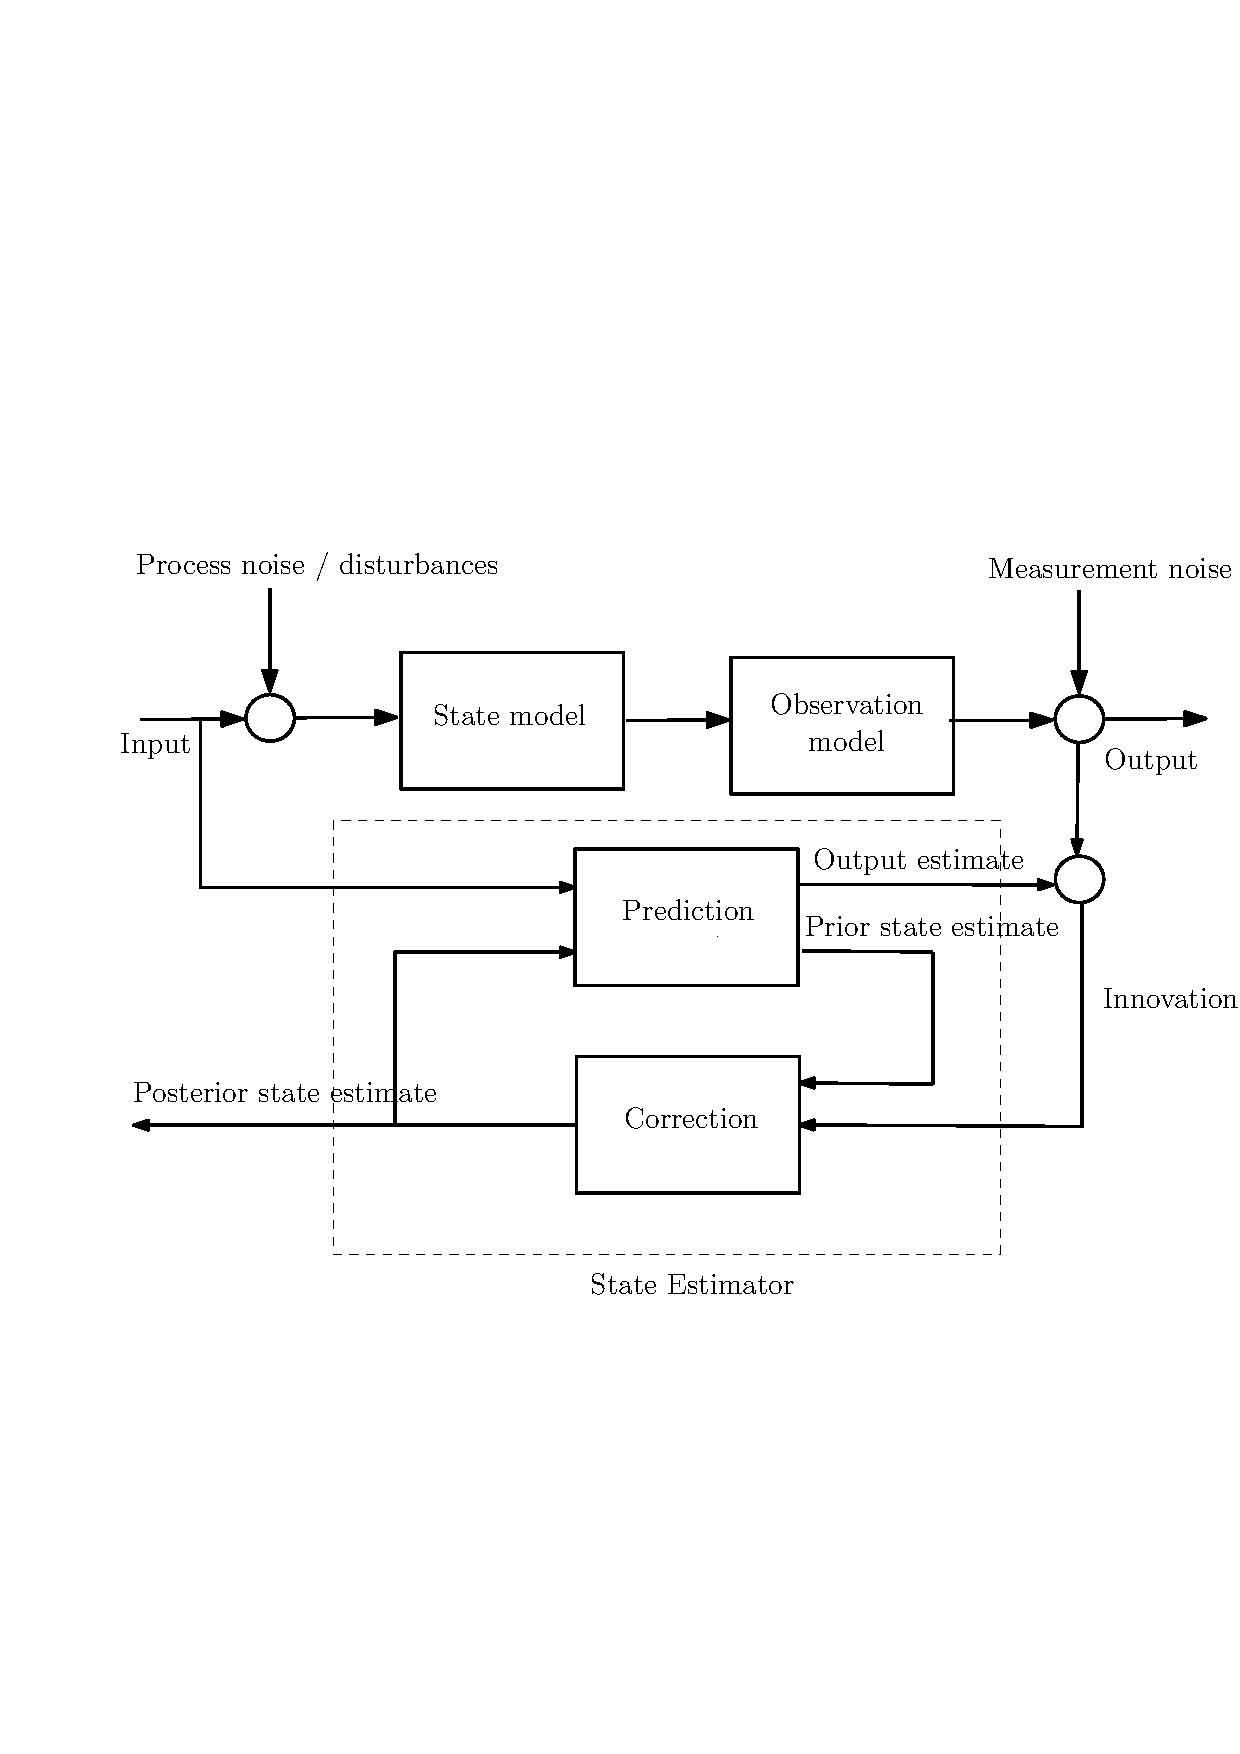
\includegraphics[width=7in]{images/Chap1_state_est_block}
	\caption{Block diagram of a state estimator}
	\label{Fig:state_estimator}
\end{figure}
Initial applications of filtering included satellite orbit determination, aircraft navigation and tracking \cite{kutsurpfi19}. More recently, filtering has found applications in diverse areas such as machine learning \cite{bishop06}, queueing networks, mathematical finance \cite{brihan08} and data assimilation problems for weather forecasting \cite{eve94}. \anand{A simple example may be good here.}

When the system dynamics are linear and the noise quantities are Gaussian, the problem is simpler and the well-known Kalman filter is the optimal solution. The Kalman filter gives a linear SDE (stochastic differential equation) for the conditional mean of the state and a Riccati type ODE for the state covariance. These two quantities However, in practice, the linear state dynamics - Gaussian disturbances assumption is often violated.  For example, in weather forecasting the states evolve via a complex system of fluid mechanics equations that are nonlinear. The optimal solution is given by a set of SDEs, like the Zakai's equation or the Kushner-Stratonovich equation. The posterior estimates are in the form of conditional distributions of the state, given the entire history of observations. A detailed discussion of the nonlinear filtering theory can be found in \cite{baicri08}. 

Linear approximations like the extended Kalman filter (EKF) were studied for application to nonlinear systems. They perform well as long as the state or observation dynamics do not deviate significantly from linearity. Later with the advent of modern computing, Monte Carlo based methods like the conventional bootstrap particle filter gained popularity. The underlying principle here is to approximate the posterior distribution using empirical samples called particles. Budhiraja et al. \cite{budchelee07} provide a comprehensive survey of numerical methods for nonlinear filtering problems. 

The main focus of this dissertation is a class of controlled particle system algorithms called the feedback particle filter (FPF). Feedback particle filter was originally formulated for the continuous-time nonlinear filtering problem in the Euclidean setting \cite{yanmehmey13}. They have since been extended to Riemannian manifolds and matrix Lie groups \cite{zhatagmeh16}. The FPF is similar in its feedback structure to the Kalman filter and in its empirical approximation approach to the standard particle filter. In other respects, they are significantly different. A crucial component of the FPF is the gain function, which is analogous to the Kalman gain in the Kalman filter. The optimal gain function in the FPF is obtained as the gradient of the solution to a particular version of Poisson's equation \cite{yanmehmey13, laumehmeyrag14}. Obtaining an analytical solution to the Poisson's equation is often difficult and hence, approximation is required. In this dissertation, our main focus is on developing algorithms to approximate the gain function. A detailed discussion is reserved for \Chapter{ch:filtering}. 

\subsection{Markov chain Monte Carlo (MCMC) algorithms}
\label{s:mcmc}
The second application of interest is Markov chain Monte Carlo (MCMC) algorithms. MCMC algorithms have a long history of being applied to problems in Bayesian statistics \cite{}. 

In standard Monte Carlo methods, expectation of a function $f$ of a random variable $X$ distributed according to a density $\pr$ is approximated empirically as,
\begin{equation}
 \Expect_{X \sim \pr} [f(X)] \eqdef \int_\state f(x)\pr(x) dx \approx \frac{1}{N} \sum_{i=1}^N f(X_i)
 \label{e:emp_avg} 
\end{equation}
where each $X_i$ is distributed according to $\pr$ and $N$ is sufficiently large. As is often the case, it may be difficult to generate a sequence of samples $\{X_i\}_1^N$ according to the desired target distribution $\pr$. Methodologies such as rejection sampling and importance sampling make use of an easy-to-sample surrogate distribution to sample from the original target distribution. But, if $\pr$ is high-dimensional, it is difficult to find a closely matching simple surrogate distribution. 

MCMC algorithms provide an alternative solution in this situation. They are a special class of Monte Carlo methods in which the samples $X_i$ are the states of an ergodic Markov chain. Given the target density $\pr$, the problem reduces to finding an appropriate transition kernel for a Markov chain that has $\pr$ as its invariant density. The Langevin diffusion, which is a perturbed gradient flow with respect to a potential function in continuous time, forms the basis of many such algorithms. The Gibbs algorithm \cite{tanwon87} and Metropolis-Hastings (M-H)  algorithm \cite{has70} are popular discrete-time MCMC techniques. They have been widely applied for problems in Bayesian inference, statistical physics, computation biology etc.

%MCMC algorithms are a popular means of sampling from high dimensional densities. Typically, computing expectations of functions via integration is infeasible in high dimensions and MCMC algorithms provide a method to obtain numerical approximations to the expectation. 
The asymptotic convergence of the empirical averages of the form \eqref{e:emp_avg} to the true expected value is guaranteed under general conditions by law of large numbers. The main drawback of these techniques as compared to standard Monte Carlo sampling which provides independent and identically distributed (i.i.d.) samples, is that the successive samples of the Markov chain are correlated to each other. This results is slower convergence of the algorithms. The central limit theorem states that,
\begin{equation}
\sqrt{N} \Bigl(\frac{1}{N} \sum_{i=1}^N f(X_i) - \Expect_{X \sim \pr} [f(X)] \Bigr) \overset{d}{\to} \normal(0, \asymvar^2),\qquad \text{as } N \to \infty, 
\end{equation}
where $\mathcal{N}(0,1)$ refers to the standard Gaussian distribution with mean zero and unit variance. Asymptotic variance $\asymvar^2$ is a measure quantifying the rate of convergence. Lower its value, faster is the convergence of the Markov chain to its invariant distribution and hence, the goal is to minimize it. 

Asymptotic variance can be expressed in terms of the solution to Poisson's equation \cite{ctcn}. Control variates, which are zero-mean terms added to the function $f$, have been used to reduce the asymptotic variance of the estimates without adding any bias. Henderson, in his dissertation \cite{henthesis97} notes that the best choice of control variates can be constructed using the solution to Poisson's equation. They also feature prominently in Chapter 11 of the book \cite{ctcn} with the objective of constructing reduced-variance estimators for network models. Control variates constructed using the fluid value function have been shown to produce a $100$-fold reduction in variance over the standard estimator for the KSRS queueing model in the examples considered in the book chapter. 

In this dissertation, we demonstrate that the same algorithms we propose for approximating the FPF gain function, find additional application in improving the performance of popular MCMC algorithms. 
% Section 11.2.1 and Section A.5 of CTCN, 
% Control variates - Prop 8.2.4 and Theorem A.5.4

\section{Tools Used in the Dissertation}
\label{s:tools}
Now, that the main application areas of the dissertation have been described briefly, we introduce the various tools that help us achieve our goal. In \Section{poissons_eq}, a preliminary description of the Poisson's equation, that is crucial to both our applications of interest is given.
\subsection{Poisson's equation} 
\label{s:poissons}
In its most general form, Poisson's equation is a second-order differential equation of the form,
\begin{equation*}
\generate h \eqdef - f,
\end{equation*}
where $\generate$ is a second-order differential operator. Usually, $f \in C^2$ is given and is ``centered'' by subtracting its mean. The function $h$ is unknown and is called the solution to the Poisson's equation. In Physics, the operator $\generate$ is often taken to be the Laplacian. Poisson's equation appears widely in the context of Markov chains and stochastic optimal control. In the context of a continuous-time diffusion process, the operator $\generate$ refers to the infinitesimal generator, also called the differential generator.  \anand{ If $f \equiv 0$, then $h$ is precisely harmonic functions \cite{glymey96a}}.

Poisson's equation is central to average-cost optimal control theory. In this case, $f$ is a one-step cost function and $h$ is called a relative value function. \anand{The states evolve in the form of a controlled Markov chain based on a given policy.} Relative value function gives the infinite-horizon expected cost when starting from a given state under this stationary policy. Approximate solutions to the equation lead to direct performance bounds of the control algorithm \cite{ctcn}. Explicit bounds on the solution $h$ have been obtained under general conditions of the chain in \cite{}.
% measure of long-term system performance in \cite{brabar96}.

Our interest lies in a particular version of Poisson's equation associated to the Langevin diffusion process. Langevin diffusion is discussed in greater detail in \Section{s:langevin_diffusion} and \Section{s:langevin_mcmc}. Gradient of the solution to this equation is the optimal choice of the gain function associated with the FPF \cite{yanmehmey13}. In MCMC algorithms, as noted by Henderson \cite{henthesis97} and later by Dellaportas et al. \cite{delkon12}, the optimal control variates can be constructed from this solution. Thus, Poisson's equation and its solution are central to the goals of this dissertation. 

Obtaining a closed form solution is difficult outside of special cases and this motivates the study of approximation algorithms. Various approaches have been studied such as the Markov semigroup approximation by Taghvaei et al. \cite{tagmeh16a}. Finding an approximate solution falls within the framework of reinforcement learning and in particular, temporal difference (TD) learning. In this dissertation, we develop variants of the TD learning algorithm that can approximate the gradient of the solution to Poisson's equation directly.

% basis for much of ergodic theory of Markov chains \cite{ctcn}


\subsection{Reinforcement learning and TD learning}
\label{s:rl_td}
In this section, a beginner level introduction to reinforcement learning algorithms is provided. Reinforcement learning algorithms have gained popularity over the last decade having achieved major successes in a wide variety of applications like AlphaGo, backgammon etc. \anand{need references} In a general setting, such algorithms involve learning what actions to take in a given situation, so as to maximize a numerical reward (or equivalently minimize a numerical cost) over a (possibly infinite) time-horizon. The learned set of actions, called a policy is a mapping from the state space to the action space. In a stochastic setting, this mapping is expressed in terms of probability of taking a particular action in a given state. The learning is performed purely based on interactions with the environment without any prior knowledge of the system model. A whole variety of algorithms including Q-learning \cite{watday92a} and temporal difference (TD) learning \cite{sut88} belong to this category. A slightly different class of algorithms that makes use of model information also exists, called approximate dynamic programming. \anand{needs rephrasing}
Although, the end objective is to obtain optimal policies, a central theme in all these algorithms is value function approximation. This aspect is what makes these algorithms an attractive choice for our objective. 

Sutton and Barto write in their monograph \cite{sutbar98}, ``If one had to identify one idea as central and novel to reinforcement learning, it would undoubtedly be temporal difference learning''. Originally introduced by Sutton in \cite{sut88}, TD learning algorithms address the problem of policy evaluation associated with discrete-time stochastic optimal control problems called Markov decision processes (MDPs). In other words, for a given fixed policy, the algorithm computes estimates of the value function through an iterative procedure. A large body of prior research is available that studies the asymptotic convergence properties of these algorithms. Most of them, however are restricted to either the discounted-cost case or an undiscounted-cost (average-cost) setting for a finite state space Markov chain with an absorbing state. Both these assumptions are violated in the context of approximating the solution to Poisson's equation of interest to us. Hence, the need to develop new algorithms. 

A least-squares approach to TD learning, introduced by Bradtke et al. \cite{brabar96},  has been discussed in the context of value function estimation for a fixed policy in \cite{ctcn}. An appropriate learning objective is chosen based on the context. For example, in optimal control, the goal is to optimize performance over the class of policies, whereas in MCMC, minimizing the asymptotic variance is the chosen criterion. Least squares TD (LSTD) learning aims to obtain approximations to the true value function from within a parameterized family of functions. The learning problem is thus reduced to finding the best approximation based on a chosen criterion from within this class. Section 11.5.2 of \cite{ctcn} presents the LSTD learning algorithm for the discounted-cost problem. Recursive update rules are presented for the parameter weights and they have been shown to converge asymptotically to the optimal values. In Section 11.5.4, the results are generalized to the average-cost setting, which requires solving the Poisson's equation. However, the application of LSTD algorithm in this case is justified only if a regenerating state for the Markov chain exists. This rules out its application to state spaces in higher dimensions.

In this dissertation, we follow the key ideas presented in Section 11.5.2 to develop a new class of algorithms called differential LSTD learning that approximates the gradient of the solution to Poisson's equation directly.  The algorithm design enables the construction of a Monte Carlo based technique that scales well in high dimensions. This is achieved by introducing an implicit discounting factor, that ensures the existence of a regenerating state for the process. For the special case of Langevin diffusion, using the self-adjoint property of the differential generator, we obtain a simple and elegant version of the algorithm in \Section{s:diff_td_langevin}.  A more general version of the algorithm that can be applied to any continuous-time diffusion processes is presented in \Section{s:diff_td_learning}. 
A similar algorithm for discrete-time examples with applications to optimal control is presented by Devraj et al \cite{devmey16arXiv}.
 
% nonlinear parameterization in Section 11.5.3 
% average-cost TD learning based on \cite{kontsi03a}
\subsection{Reproducing kernel Hilbert space (RKHS)}
\label{s:rkhs}
Traditionally, TD learning has been tested on spaces spanned by a carefully chosen finite set of basis functions. However, there are no standard approaches to choosing the basis.  If any insight about the structure of the true value function is available, this can be exploited in choosing an appropriate function class. In optimal control problems, this insight is available in the form of fluid value functions. But this is not true for Poisson's equation of interest. One of the novelties of this dissertation is the use of reproducing kernel Hilbert space (RKHS) as an approximating function space for TD learning algorithms. This simplifies the choice of problem dependent basis functions by making use of the information about particle locations effectively. 
 
Reproducing kernel Hilbert spaces form an important class of function spaces in learning theory \cite{aro50, schsmo01}. They are complete Hilbert spaces uniquely characterized by a kernel function. The use of RKHS for function approximation provides us with greater flexibility and potentially a richer function class. Although optimization in an RKHS is typically infinite dimensional, they are endowed with useful properties that help us reduce the problem to finding a finite set of parameters via the representer theorem \cite{kimwah71, schhersmo01}. A brief background of the RKHS theory along with properties that make them useful in this dissertation is provided in \Chapter{ch:rkhs}. The differential TD learning algorithm specific to the Langevin diffusion is adapted to accommodate an RKHS as the approximating function space in \Chapter{ch:rkhs}.
 

\section{Dissertation Outline}
\label{s:outline}
The various topics discussed in this chapter may seem distinct and disconnected. This dissertation attempts to tie them together as it progresses. To summarize, we restrict our attention to approximating solutions of a particular version of the Poisson's equation. Differential TD learning algorithms using a finitely parameterized family of functions and an RKHS are studied and presented. Approximations obtained using these algorithms are tested and have been shown to improve the performance of the FPF and MCMC algorithms. 

The main contributions of this dissertation that form the remaining chapters can be summarized as - i) development of differential LSTD learning algorithm, similar to LSTD in \cite{ctcn} to approximate the gradient of the solution to Poisson's equation directly in \Chapter{ch:diff_td}, ii) refinement of this algorithm with a simpler resolution \cite{radmey18a} in \Section{s:diff_td_langevin}, iii) address the problem of basis selection by the use of RKHS in Chapter \ref{ch:rkhs}, iv) applications to nonlinear filtering in \Chapter{ch:filtering} and MCMC algorithms in \Chapter{ch:mcmc}. Finally, conclusions and scope for future work are included in Chapter 6.  

\section{Notation}
\label{s:notation}
$\bfmX\eqdef \{X_t: t\ge 0\}$ is a stochastic process, evolving on the state space  $\state$, which is taken to be $\Re^d$, unless specified. A subscript notation $X_t$ is often used to denote $X(t)$, where $t$ is an index of time. The symbol $\pr$   denotes a probability density on $\state$, and $L^2(\state,\pr)$ is the Hilbert space of square integrable functions with the usual inner product,
$\langle \phi,\psi\big\rangle_{L^2}\eqdef\int\phi(x)\psi(x) \pr(x)\ud x$, where $\phi$ and $\psi$ are scalar valued functions in $L^2(\state, \pr)$;
written $L^2$ when there is no risk of ambiguity.  The associated norm is
denoted   $\|\phi\|^2_{L^2}\eqdef\langle\phi,\phi\rangle_{L^2}$. The inner product is extended to vector valued functions $f,g: \state \to \Re^d$ by defining, $\langle f, g \rangle_{L^2} \eqdef \sum_{k=1}^d \langle f_k, g_k \rangle_{L^2}$. The expectation of a function $f$ with respect to $\pr$ is written as $\Expect_{X \sim \pr}[f(X)]$ and the  notation $\Expect_x$ is used as shorthand for the conditional expectation $\Expect_x[f(X_t)] \eqdef \Expect[f(X_t)|X_0 = x]$.  We use $\|\cdot\|$ without the subscript to refer to the Euclidean norm and $\|\cdot \|_\infty$ refers to the maximum or uniform norm. 

Another Hilbert space $\clH$ will appear in the application of reproducing kernel Hilbert space theory with its inner product denoted   $\langle \varble, \varble \rangle_{\clH}$,  and induced norm    $\| \varble \|_\clH$. $C^k$ is used to denote the space of $k$-times continuously differentiable functions $f\colon\state\to\Re$,
$\nabla f $ denotes the gradient of a function $f\in C^1$, and $\Delta f$ the Laplacian for $f\in C^2$. If $\state = \Re$, the notation $f'$ and $f''$ are often used to denote the first and second derivatives respectively.

%The remainder of the dissertation is organized as below. In Chapter \cite{}, we discuss the problem set up, i.e. the Poisson's equation for Langevin diffusions and introduce differential TD learning} to obtain approximate solutions. A simpler resolution to the problem is proposed and an algorithm derived using this resolution is presented in Chapter \cite{}. In Chapter \cite{}, we discuss the application to nonlinear filtering in detail along with some numerical results. The second application to MCMC algorithms is presented with numerical examples in Chapter \cite{}. Finally, we present conclusions and scope for future work in Chapter \cite{}. 
 


 

%\begin{figure}[htbp]
%  \centering
%    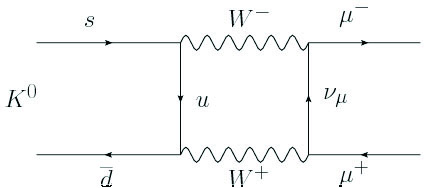
\includegraphics[width=5in]{images/diagram}
%    \caption[EPS format diagram. Note: no filetype is designated by adding an extension.]{EPS format diagram. Note: no filetype is designated by adding an extension. The file type is determined and the correct procedure is automatically chosen by xelatex.}
%\end{figure}
%
%
%
%\begin{figure}[htbp]
%     \centering
%   \mbox{
%      \subfigure [] {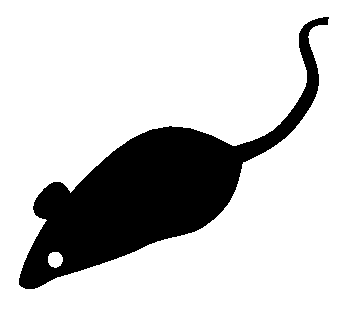
\includegraphics[scale=0.6]{images/mouse}} \qquad
%      \subfigure []{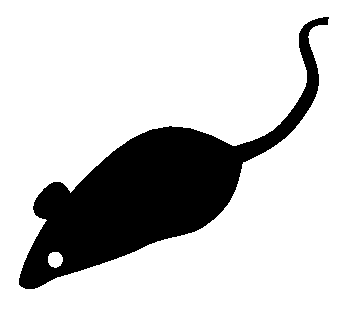
\includegraphics[scale=0.6]{images/mouse}} \qquad
%     }
%    \mbox{
%      \subfigure [] {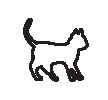
\includegraphics[scale=3]{images/cat}} \qquad
%      \subfigure [] {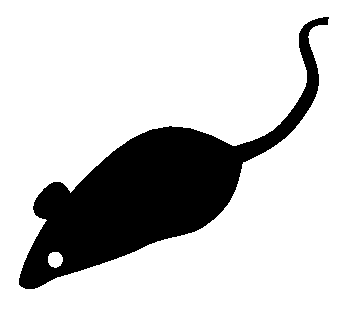
\includegraphics[scale=0.6]{images/mouse}} \qquad
%      }
%    \caption[Tom and Jerry]{Tom and Jerries. This caption demonstrates how the sub-captions are left out of the List of Figures, but included in the figure itself. A) Tom the first; B) Tom the second; C) Jerry; D) Tom the third.}
%    \label{mice}
%  \end{figure}


\chapter{Differential TD learning} %\footnote{Published as \cite{raddevmey16}}
\label{ch:diff_td}
A basic introduction of the essential elements of this dissertation was provided in \Chapter{ch:intro}. In this chapter, a more formal mathematical description of the concepts is aimed at. The outline of this chapter is:
\begin{romannum}
\item In \Section{s:langevin_diffusion}, a prerequisite introduction to the Langevin diffusion and its associated Poisson's equation is given. The intention is to provide motivation as to why solving this equation is important to the two applications of interest.
\item The standard least squares temporal difference (LSTD) learning algorithm is described. This algorithm forms the basis of techniques to approximate the solution to Poisson's equation. A detailed derivation is presented, as a precursor to deriving a new variant.
\item We derive the differential LSTD ($\gradTD$) learning algorithm that tries to approximate the gradient of the solution to Poisson's equation directly rather than the function itself.
It is shown in \Section{s:diff_td_langevin}, that in the special case of Langevin diffusion, the $\gradTD$ algorithm provides a simple and elegant solution. This is achieved by using the self-adjoint property of its differential generator. This is the major contribution in this chapter. 
\item A more general version of the algorithm, that can be applied to a broad class of continuous-time diffusion processes is also derived along the lines of the standard LSTD algorithm. This algorithm with its application to gain function approximation in the FPF was published as a conference proceeding \cite{raddevmey16}. A discrete-time analog of the algorithm has been successfully applied to problems in optimal control. 
\end{romannum}
% cite the paper as a foot note.
 %along the lines of the LSTD algorithm described in Section 11.5.2 in \cite{ctcn}

\section{Langevin Diffusion and Poisson's Equation}
\label{s:langevin_diffusion}
In this section, we introduce the Langevin diffusion with only the requisite amount of detail, so that the broad motivation is not obfuscated by technical details. A more elaborate discussion is reserved for \Section{s:langevin_mcmc} in the context of MCMC algorithms. %\anand{minor}

\subsection{Langevin Diffusion}

The Langevin diffusion may be regarded as  a $d$-dimensional gradient flow perturbed with ``noise'',  described by  the SDE,
\begin{equation}
\ud \markovstate_t = \underbrace{- \nabla \pot(\markovstate_t) \, \ud t}_{\text{drift}}+  \underbrace{\sqrt{2} \, \ud W_t}_{\text{diffusion}},
\label{e:langevin_cts}
\end{equation}
where $\bfmW=\{W_t : t\ge 0\}$ is a standard Brownian motion on $\Re^d$. The potential function $U:\state \to \Re$ is continuously differentiable. 
Under suitable regularity conditions, this diffusion is reversible and has a unique invariant density $\pr=e^{-\pot+\Lambda}$, where $\Lambda$ is a normalizing constant so that $\pr$ integrates to unity \cite{bha82}. The SDE in \eqref{e:langevin_cts} can be thought of as composed of a deterministic drift term and a stochastic diffusion term. The intuition is that the drift term moves the process along the direction in which the density $\pr$ increases. In this sense, it is a biased random walk. In practice, as simulating path solutions to this SDE is difficult, discretized versions of the equation based on Euler-Mauryama scheme are used \eqref{e:langevin_discrete}:
\begin{equation}
\markovstate_n = \markovstate_{n-1} - \nabla U(\markovstate_{n-1}) \mcmcstep_{n} + \sqrt{2  \mcmcstep_{n-1}} W_{n-1} ,
\label{e:langevin_discrete}
\end{equation}
where $\{\mcmcstep_n\}_{n\geq 1}$ is a sequence of step sizes and $\{W_n\}_{n\geq 1}$ is a sequence of i.i.d. standard Gaussian random variables.  In this dissertation, only implementations using a constant step size parameter $\mcmcstep_{n} \equiv \mcmcstep$ are considered. 
 
% The Markov transition kernel of the diffusion process converges to a unique invariant density $\pr=e^{-\pot+\Lambda}$ in total variation \cite{robtwe96} or Wasserstein distance \cite{bolgengui11},  where $\Lambda$ is a normalizing constant so that $\pr$ integrates to unity. 
% admits a strong solution $\{\markovstate_t\}_{t\geq0}$, 

The Langevin diffusion is associated with a differential generator $\generate$ (also called infinitesimal generator), which is defined as,
\begin{equation}
\begin{aligned}
\generate f &:= \lim_{t \to 0} \frac{\Expect [ f(\markovstate_t) - f(x) | \markovstate_0 = x]}{t} \\
& = -\nabla \pot \cdot \nabla f + \Delta f,\qquad f\in C^2,
\label{e:langevin_generator}
\end{aligned}
\end{equation}
where $\nabla$ denotes the gradient and $\Delta$ is the Laplacian. The differential generator can be thought of as the derivative operator in an expected sense. Under conditions on $U$, this SDE defines a strong Markov semigroup $\{P_t\}_{t \geq 0}$. The generator $\generate$ can be written in terms of the semigroup as,
\begin{equation}
\generate = \lim_{t \to 0} \frac{P_t - I}{t}.
\label{e:lang_generate_semigroup}
\end{equation}

\subsection{Poisson's Equation}
Let $c \colon \state \to \Re$ be a function of interest, and 
\begin{equation}
\eta := \Expect_{\markovstate \sim \pr}[c(\markovstate)] =  \int_\state c(x) \pr(x) \ud x = \langle c, 1 \rangle_{L^2}.
\end{equation}
A function $h\in C^2$ is said to be the solution to Poisson's equation with forcing function $c$ if it satisfies,
\begin{equation}
\generate h := - \tilc, \qquad  \tilc = c - \eta.
\label{e:poissons}
\end{equation}
Additionally, $h$ can also be expressed in the following integral form:
\begin{equation}
h(x) =\int_0^\infty \Expect_x[\tilc(\markovstate_t)] \ud t,
\end{equation}
where $h(x)$ can be interpreted as the infinite-horizon expected normalized cost with the initial state $\markovstate_0 = x$. The notation $\Expect_x[\tilc(\markovstate_t)]$ is shorthand for the conditional expectation $\Expect[\tilc(\markovstate_t)|\markovstate_0 = x]$, with $x$ as the initial state. The function $h$ is also called the relative value function in average-cost optimal control.  

The existence of a solution $h$ in a weak sense holds under very weak assumptions on $\pot$ and $c$  \cite{glymey96a,konmey12a}.  Glynn et al. in \cite{glymey96a} provide Lyapunov bounds for the solution $h$.  Representations for the gradient of $h$ and its bounds are obtained in \cite{laumehmeyrag15,devkonmey17b}.   The existence of  a  smooth solution $h\in C^2$ has been established under stronger conditions in \cite{parver01}, subject to growth conditions on $c$ similar to those used in  \cite{glymey96a}. In the remaining part of this dissertation, existence of $h$ is assumed. 
% \cite{makshw - Makowski Schwartz - On the Poisson equation for Countable Markov chains}

Analogous to $h$, a discounted-cost value function $h^\discount$ is defined as,
\begin{equation}
h^\discount(x) := \int_0^\infty \exp(-\discount t )\Expect_x[c(\markovstate_t)] \ud t, 
\label{e:discount_value_fn}
\end{equation}
with a discount rate $\discount  >0$ and $c(x)$ is the one-step cost function at the state $x$. The discounted-cost value function is often more popular in applications where the future costs incurred are assigned lower weights than the immediate costs. It may be noted that as the value of $\discount \to 0$, it closely approximates an average-cost problem. 

\subsection{Relevance to our Applications} 
The solution $h$ of Poisson's equation associated to the Langevin diffusion \eqref{e:poissons} is crucial in each of the applications we consider in this dissertation. In the feedback particle filter (FPF), the innovations gain function $\kFPF$ at each $t$ is obtained as  the gradient of $h$ \cite{yanmehmey13}:
\begin{equation}
\kFPF (x) = \nabla h(x)\, ,  \quad x\in\state\, .
\label{e:fpfgain}
\end{equation}
A detailed analysis of the Poisson's equation appearing in the FPF is performed in \cite{laumehmeyrag15}. The FPF is described in detail in Chapter 4. %\Chapter{ch:filtering}.

In MCMC algorithms, as mentioned in \Chapter{ch:intro}, the asymptotic variance is a measure of convergence. In this context, $\pr$ is the target density, and $c$ is the function whose expectation needs to be computed. The expected value is approximated using the empirical mean $\eta_N$:
\begin{equation} \eta_N := \frac{1}{N} \sum_{n=0}^{N-1} c\,(\markovstate_n),\end{equation}
where $\markovstate_n \sim \pr$, is obtained by sampling from an ergodic Markov chain with $\pr$ as its invariant density. One such Markov chain is the discretization in \eqref{e:langevin_discrete}, also known as the unadjusted Langevin algorithm (ULA) or Langevin Monte Carlo (LMC). Under general conditions, the mean estimates will obey a Central Limit Theorem (CLT) of the form,
\begin{equation}
\sqrt{N} \Bigl( \eta_N - \eta \Bigr) \overset{d}{\to} \normal(0,\asymvar ^2),
\end{equation}
where the convergence is in distribution \cite{MT,bha82}. Here, $\asymvar^2$ denotes the asymptotic variance that has a representation in terms of $h$ \cite{glymey96a,MT,asmgly07}. It has been noted in \cite{henthesis97, delkon12} that estimates for the solution $h$ can be used to construct algorithms that provide estimators with improved asymptotic variance. More details about the application to MCMC algorithms is in \Chapter{ch:mcmc}. 

Computation of $h$ is typically intractable, especially in higher dimensions and hence, approximation approaches are required. Algorithms based on reinforcement learning provide a suitable approach. \Section{s:lstd} reviews the least-squares TD (LSTD) learning algorithm that attempts to obtain the best approximation in an $L^2(\pr)$-norm sense. The LSTD algorithm has limitations, which curtails its scope in using it for our applications. To overcome this, a novel class of algorithms, called the differential LSTD ($\gradTD$) learning, based on the idea of approximating the gradient of the solution to Poisson's equation directly is proposed. The algorithm for the case of Langevin diffusion is derived in \Section{s:diff_td_langevin}.  A more general version is discussed in \Section{s:diff_td_learning}. 

\section{Least Squares Temporal Difference (LSTD) Learning} 
\label{s:lstd}
\subsection{LSTD for discounted cost value function}
In this section, the least squares temporal difference (LSTD) learning algorithm to approximate the discounted-cost value function \eqref{e:discount_value_fn} of a continuous-time diffusion process is presented.  Theory for TD learning in the discounted cost setting is largely complete, however theory and algorithms for the average cost case is more fragmented. The LSTD algorithm was first proposed for a finite-state-action space Markov decision process (MDP) in the context of stochastic optimal control  by Bradtke et al. in \cite{brabar96}.  It is noted in \cite{brabar96, boy02} that the LSTD algorithm, although more computationally expensive than the conventional TD learning algorithm of Sutton \cite{sut88}, are statistically more efficient and also avoids the choice of a tunable step-size parameter. 

The derivation of the algorithm here closely follows the one in Section 11.5.2 in \cite{ctcn}. The key difference is that the book section discusses the discrete-time case.  Consider a one-dimensional continuous-time diffusion on $\Re$:
\begin{equation}
\ud \markovstate_t = a(\markovstate_t) \ud t + \sigma(\markovstate_t) \ud B_t,
\label{e:cts_diffusion}
\end{equation}
where $\bfmB$ is standard Brownian motion and $a : \Re \to \Re$ is a Lipschitz-continuous function. The differential generator $\generate$ is defined for functions $f:\Re \to \Re$ as: 
\begin{equation}
\generate f = a f' + \frac{\sigma^2}{2} f'', \qquad f \in C^2.
\label{e:diffusion_generator}
\end{equation}
It may be noted that the Langevin diffusion \eqref{e:langevin_cts} is a special case of the diffusion \eqref{e:cts_diffusion} with $a(x) = -\grad U(x)$ and $\sigma(x) \equiv \sqrt{2}$, and the associated differential generator is defined in \eqref{e:langevin_generator}. 

Consider a parameterized family of approximations $\{h^\param : \param \in \Re^\ell\}$. In the case of a linear parameterization, where we have $\ell$ functions on $\state$ as the basis, denoted $\{\basis_i : 0 \leq i \leq \ell\}$, the parameterized family $\{h^\param\}$ becomes,
\begin{equation}
h^\param(x) := \sum_{i=1}^\ell \param_i \basis_i(x) = \param^\transpose \basis(x), \qquad x \in \state
\label{e:linear_param}
\end{equation}
The goal in LSTD learning algorithm is to minimize the approximation error in $L^2(\pr)$ norm:
\begin{equation}
\begin{aligned}
\error(\param) &:=  \| h^\discount - h^\param \|^2_{L^2} \\
& = \int_\state (h^\discount(x) - h^\param(x))^2 \pr(x) \ud x \\
& = \Expect_{\markovstate \sim \pr} [|h^\discount(\markovstate) - h^\param(\markovstate)|^2].
\label{e:h_norm_error}
\end{aligned}
\end{equation}
Among the conventional TD algorithms, only TD($1$) has an interpretation as a norm minimization problem. It is evident from the definition of $\error(\param)$ that it penalizes the approximation error more strongly for states with larger invariant probability $\pr(x)$. As noted in \cite{ctcn}, these are the states that are visited more often and hence, a better approximation of $h^\discount$ is desired at these points on $\state$. A more important benefit of using the $L^2(\pr)$ norm is that it allows the construction of an algorithm using Monte Carlo methods. 

The necessary conditions for optimality can be obtained by taking the gradient of \eqref{e:h_norm_error} with respect to $\param$ and equating it to zero, 
\begin{equation}
\begin{aligned}
0 &= - \nabla_\param \error(\param)\\
& = 2 \|(h^\discount - h^\param) \nabla_\param h^\param \|_{L^2} \\
& = 2 \Expect_{\markovstate \sim \pr} [(h^\discount(\markovstate) - h^\param(\markovstate)) \nabla_\param h^\param(\markovstate)]
\end{aligned}
\label{e:first_order_condition}
\end{equation} 
	\anand{Need to verify if the exchange of derivative and expectation is valid for a nonlinear parameterization}
In general, a solution to \eqref{e:first_order_condition} can be obtained using recursive updates of the parameter $\param$ by stochastic approximation techniques. However, for the linear parameterization \eqref{e:linear_param}, the optimal $\param^*$ admits a closed form expression:
\begin{equation}
\param^* := M^{-1} b,
\label{e:param_opt_lstd}
\end{equation}
where $M$ and $b$ are defined as,
\begin{equation}
M: = \Expect_{\markovstate \sim \pr} [\basis(\markovstate) \basis(\markovstate)^\transpose], \qquad b:= \Expect_{\markovstate \sim \pr} [h^\discount(\markovstate) \basis(\markovstate)].
\label{e:lstd_M_b}
\end{equation}
The expression for $b$ is not computable as it involves the unknown function $h^\discount$ that we are trying to approximate. The challenge now is to find an alternate observable representation for $b$. 

A resolution is obtained using the definition of $h^\discount$ \eqref{e:discount_value_fn} and the generalized resolvent kernel of \cite{nev72,meytwe93e,devkonmey17a}: For a measurable function $G\colon\Re\to\Re$, and measurable functions $f$ in some domain, the resolvent kernel $R_G$ is an operator defined as,
\begin{equation}
R_G f\, (x) := \int_0^\infty \Expect_x\Bigl[ \exp\Bigl(-\int_0^t G(\markovstate_s)\, \rmd s \Bigr) f(\markovstate_t)\Bigr] \ud t.
\label{e:resolvent_neveu}
\end{equation}
In  \cite{nev72,meytwe93e} it is assumed that $G>0$ everywhere. These conditions are relaxed in \cite{konmey03a,devkonmey17a}. An adjoint operator $R^\dagger_G$ is defined such that the following holds:
\begin{equation}
\langle R_G f,\, g \rangle_{L^2} = \langle f ,\, R^\dagger_G g \rangle_{L^2}, 
\label{e:RG_adjoint}
\end{equation}
where $f$ and $g$ are in $L^2(\pr)$. 
%In these papers, it is shown that $R_G$ is a right inverse of $[I_G -\clD]$ on some domain, i.e.,
%\begin{equation*}
%[I_G-\clD]R_G f = f,
%\end{equation*}
%where the operator $I_G$ represents multiplication by the function $G$. 

The discounted-cost value function $h^\discount$ in \eqref{e:discount_value_fn} can now be represented in terms of $R_G$ \eqref{e:resolvent_neveu} with $G \equiv \discount$ as,
\begin{equation}
h^\discount = R_\discount c.
\label{e:lstd_hgamma_resolvent}
\end{equation}
If the value function $h^\discount$ is $C^2$, then it solves the discounted-cost optimality equation,
\begin{equation}
\discount h^\discount - \generate h^\discount =  c.
\label{e:dcoe}
\end{equation}
This is analogous to the Poisson's equation that arises in the average-cost case. 
Using \eqref{e:lstd_hgamma_resolvent} and \eqref{e:dcoe}, resolvent kernel $R_\discount$ can be shown to satisfy the following inverse formula:
\begin{equation}
R_\discount c = ( I_\discount - \generate)^{-1} c,
\end{equation}
where $I_\discount$ refers to multiplication by $\discount$. The inverse $(I_\discount - \generate)^{-1}$ exists on some domain under conditions provided in \cite{devkonmey17a}.  
%Multiplying $h^\discount$ by $\basis$, we get,
%\begin{equation}
%\begin{aligned}
%h^\discount (x) \basis(x) &=  \Bigl(\int_0^\infty \exp(-\discount t )\Expect_x[c(\markovstate_t)] \ud t \Bigr) \basis(x) \\
%&= \int_0^\infty \exp(-\discount t) \Expect_x[c(\markovstate_t) \basis(\markovstate_t)] \ud t
%\label{e:discount_hpsi}
%\end{aligned}
% \end{equation}
The following transformation can be applied to $b$, using \eqref{e:lstd_hgamma_resolvent} followed by an adjoint trick,
\begin{equation}
\begin{aligned}
b = \Expect_{\markovstate \sim \pr} [h^\discount(\markovstate) \basis(\markovstate) ] &= \langle h^\discount, \, \basis \rangle_{L^2}\\
& = \langle R_\discount c, \,\basis \rangle_{L^2} \\
& = \langle c,\, R^\dagger_\discount \basis \rangle_{L^2},
\label{e:lstd_b_R_adjoint}
\end{aligned}
\end{equation}
where $R^\dagger_\discount$ denotes the adjoint of $R_\discount$. Now, all that remains is to obtain an expression for the adjoint operator $R^\dagger_\discount$ in terms of observable quantities. This is achieved by the application of \Lemma{lemma:R_adjoint}.

\begin{lemma}
\label{lemma:R_adjoint}
Let $\bfPhi=\{\markovstate_t : t\in\Re\}$ denote a stationary version of a continuous-time diffusion process.
For measurable functions $f,g$ with at most exponential growths we have,
\begin{equation}
\langle R_\discount f, \, g \rangle_{L^2}   =  \langle f, \, R_\discount^\dagger g \rangle_{L^2} =  \Expect_{\markovstate \sim \pr} [ f(\markovstate_t)	\eligibvector_g(t)   ]\,, \quad t\in\Re,
\label{e:LSTD_adjoint}
\end{equation}
wherein $\bfvarphi_g$ is the stationary process:
\begin{equation}
%\eligibvector_g(t)
%=
%\int_{-\infty}^t  \exp(-\discount (t-r)) g(\markovstate_r)   \,  \ud r
\eligibvector_g(r) \eqdef \int_0^\infty \exp(-\discount (t -r)) g(\markovstate_{r-t}) \ud t,
\label{e:LSTD_eligib_integral}
\end{equation}
Consequently, 
\begin{equation}
R_\discount^\dagger g(x) = \Expect [\eligibvector_g(t)|\markovstate_t=x]
\end{equation}
\end{lemma}

\begin{proof}
 This is achieved by applying the stationarity property of the process $\markovstate_t$, which gives, 
\begin{equation}
\Expect_{\markovstate \sim \pr}[f(\markovstate_t) g(\markovstate_0)] = \Expect_{\markovstate \sim \pr} [f(\markovstate_0) g(\markovstate_{-t})].
\end{equation} 
The proof is obtained by rewriting $b$ in its integral form as,
\begin{equation}
\begin{aligned}
\langle R_\discount f, \, g \rangle_{L^2} 
& = \int_0^\infty \exp(-\discount t)  \Bigl(\int_{\state} \Expect[f(\markovstate_t)| \markovstate_0 = x] g(x)  \pr(x) \ud x \Bigr) \ud t \\
& = \int_0^\infty \exp(-\discount t)  \Bigl(\int_{\state} \Expect[f(\markovstate_t) g(\markovstate_0)| \markovstate_0 = x]  \pr(x) \ud x \Bigr) \ud t \\
& = \int_0^\infty \exp(-\discount t) \Expect_{\markovstate \sim \pr}[f(\markovstate_t) g(\markovstate_0)]\ud t \\
& = \int_0^\infty \exp(-\discount t) \Expect_{\markovstate \sim \pr}[f(\markovstate_0) g(\markovstate_{-t})] \ud t \qquad \text{(Applying the stationarity property of $\markovstate$)}\\
& = \Expect_{\markovstate \sim \pr}\Bigl[f(\markovstate_0) \underbrace{\int_0^\infty \exp(-\discount t) g(\markovstate_{-t})\ud t}_{\eligibvector_g(0)}\Bigr]  \qquad \text{(Applying Fubini's theorem and absolute integrability)}\\
& = \langle f, R^\dagger_\discount g\rangle_{L^2}.
\label{e:lstd_resolution}
\end{aligned}
\end{equation}
It can be seen from \eqref{e:lstd_resolution} that the adjoint $R^\dagger_\discount$ operating on a function $g$ in $L^2(\pr)$ takes the form:
\begin{equation}
R^\dagger_\discount g(x) \eqdef \int_0^\infty \exp(-\discount t ) \Expect_x[g(\markovstate_{-t})] \ud t %\qquad \text{\anand{Needs verification}}
\end{equation}
\end{proof}
Thus, the adjoint $R^\dagger_\discount$ can be interpreted as the resolvent for the time-reversed process $\{\markovstate_{-t}\}$. 
If we denote $\eligibvector_\basis$ as,
\begin{equation}
\eligibvector_\basis(r) \eqdef \int_0^\infty \exp(-\discount (t -r)) \basis(\markovstate_{r-t}) \ud t,
\label{e:lstd_eligib}
\end{equation}
$b$ in \eqref{e:lstd_b_R_adjoint} can be written as,
\begin{equation}
b = \Expect[c(\markovstate_0) \eligibvector_\basis(0)].
\label{e:lstd_b}
\end{equation}
% \ section{Galerkin approximation}
The function $\eligibvector_\basis$ is called the eligibility vector in TD learning. A slightly more general proof using the generalized resolvent kernel $R_G$ appears in the derivation of $\gradTD$ learning in \Section{s:diff_td_learning}.

This representation for $b$ \eqref{e:lstd_b}, combined with the representation for $M$ in \eqref{e:lstd_M_b} lends itself to application of Monte Carlo methods in their computation. Monte carlo approximations to $M$ and $b$ can be obtained using the following integral forms:
\begin{subequations}
\begin{align}
M &\approx \frac{1}{T} \int_0^T  \basis(\markovstate_t) \basis^\transpose(\markovstate_t) \ud t
\label{e:lstd_M_T}
\\
b & \approx  \frac{1}{T} \int_0^T c(\markovstate_t) \eligibvector_\basis(t) \ud t
\label{e:lstd_b_T}
\end{align}
\end{subequations}
A recursive formulation of the algorithm can be provided in terms of the three ODEs:
\begin{subequations}
\begin{align}
\ddt \eligibvector_\basis (t) &= - \discount\, \eligibvector_\basis(t) + \basis (\markovstate_t) 
\label{e:lstd_ode_eligib} \\
\ddt b(t) &=  c(\markovstate_t)\eligibvector_\basis(t)
 \label{e:lstd_ode_b}\\
\ddt M(t) &= \basis(\markovstate_t) \basis^\transpose(\markovstate_t) 
\label{e:lstd_ode_M} \\
\param(t) &\eqdef  M(t)^{-1} b(t)
\label{e:lstd_theta_T}
\end{align}
\end{subequations}

\Cref{e:lstd_ode_eligib,e:lstd_ode_b,e:lstd_ode_M,e:lstd_theta_T} summarize the LSTD algorithm. The system of ODEs is initialized with $\eligibvector_\basis(0), b(0) \in \Re^\ell,$ and a positive definite $\ell \times \ell$ matrix $M(0)$. The computational complexity of $O(\ell^3)$ arising due to matrix inversion operation in \eqref{e:lstd_theta_T} can be reduced by applying the matrix inversion lemma, as pointed out in \cite{ctcn}. 

The ODE in \eqref{e:lstd_ode_eligib} that governs the evolution of the eligibility vector $\eligibvector_\basis(t)$ is equivalent to the one that appears in TD($\lambda$) algorithm \cite{sut88}, with the exponential ``forgetting factor'' $\lambda = 1$. Convergence of the parameter estimates $\param(t)$ to $\param^*$ in the limit as $t$ goes to $\infty$ has been shown by the application of law of large numbers. % exponential weighting with recency. 

A linear parameterization for $h^\param$ is not essential for the LSTD algorithm. For a nonlinear parameterization,  LSTD can be implemented as a stochastic approximation recursion. A discussion of nonlinear parameterization is skipped here and reserved for \Section{s:diff_td_learning} while discussing the differential TD learning algorithm. 

\subsection{LSTD for Poisson's equation}
\label{s:lstd_avg_cost}
The LSTD algorithm was presented in the context of approximating the discounted-cost value function in \Section{s:lstd}. To approximate the average-cost value function $h$ \eqref{e:poissons}, the common practice is to use a discounted formulation as a proxy. The discount rate $\discount$ is usually set very close to zero with the intention of mimicking the average cost problem. However, it is known the variance of the algorithm diverges as $\discount \to 0$.  In the paper by Tsitsikilis et al. \cite{tsivan99b}, a variant of the TD($\lambda$) learning algorithm for the average-cost case is presented for the case of finite state space Markov chains. It is mentioned in the conclusions that extensions to a general state space is easily possible, but it only considers the case where the exponential weighting factor $\lambda <1$. Only when $\lambda =1$, the algorithm can be interpreted as minimizing the $L^2(\pr)$ norm of the approximation error $\error$ \eqref{e:h_norm_error}. 

The LSTD algorithm for the average cost case, that involves the Poisson's equation is also discussed in Section 11.5.4 of \cite{ctcn}. However, this algorithm yields asymptotically unbiased estimators only with the underlying assumption of the existence of a regenerating state. In informal terms, a regenerating state of a Markov chain is one that is visited infinitely often and when visited, the chain can be thought of as forgetting the past, i.e. once the regenerating state is reached, the future transitions of the chain are statistically independent from its past and hence, its entire history may be discarded. This requirement impedes the applicability of the algorithm, if the dimension of the state space is greater than one. This motivates the development of algorithms that can overcome these shortcomings in Sections \ref{s:diff_td_langevin} and \ref{s:diff_td_learning}.  

\section{Differential TD ($\gradTD$) Learning}
In this Section, we describe the differential LSTD ($\gradTD$) learning algorithm, which tries to approximate the gradient of the solution to Poisson's equation \eqref{e:poissons} directly. The development of this algorithm is motivated by two factors - i) the shortcomings of the LSTD algorithm for dimensions $>1$, and ii) applications that only require the gradient of the solution like the FPF. In conventional applications, where we are interested in $h$ instead of $\nabla h$, in addition to obtaining the optimal parameter values, we also need to add an optimal constant term. Keeping the same notation in the previous section, the goal of the $\gradTD$ learning algorithm is:
\begin{equation}
\param^* = \argmin_\param \| \grad h -\grad h^\param\|^2_{L^2}.
\label{e:gradTD_norm_error}
\end{equation}

\subsection{$\gradTD$ learning for Langevin diffusion}
\label{s:diff_td_langevin}
In this Section, we first focus on the special case of the Langevin diffusion \eqref{e:langevin_cts}. A more generic version of $\gradTD$ learning that is applicable to any continuous-time diffiusion process is described in \Section{s:diff_td_learning}. For the Langevin diffusion, a property of its differential generator \eqref{e:langevin_generator},  described in \Prop{prop:lang_generator_grad} allows the construction of a simple algorithm. The advantages of this simpler resolution will be more evident after the general version is presented in \Section{s:diff_td_learning}. \Prop{prop:lang_generator_grad} is a corollary to the following result from \cite{hwanorwu15,yanlaumehmey16} and can be proved by a simple application of the integration by parts formula:
\begin{proposition}
	\label{prop:lang_generator_grad}
	For a Langevin diffusion with differential generator $\generate$ \eqref{e:langevin_generator}, suppose that $f,g\colon\Re^d \to\Re$ are in $C^2  \cap L^2$, and that their first and second partial derivatives also lie in $L^2$. Then,
	\begin{equation}
	\langle \nabla f, \nabla g \rangle_{L^2} = \sum_{k=1}^d \Big \langle \frac{\partial f}{\partial x_k},  \frac{\partial g} {\partial x_k}\Big \rangle_{L^2}  = - \langle  f, \generate g\rangle_{L^2} = - \langle \generate f , g \rangle_{L^2}.
	\label{e:gradDual}
	\end{equation}
	\qed
\end{proposition} 
\begin{proof}[Proof]
	We can assume that $f$ and $g$ have compact support. The extension to arbitrary functions satisfying the assumptions of the proposition is obtained by approximation in $L^2(\pr)$. In the following, $\partial_k f$ is used as shorthand for $\frac{\partial f}{\partial x_k}$. \anand{What does this comment mean?} 
	
	Consider first the scalar case, where $d=1$: 
	
	\begin{equation}
	\begin{aligned}
	\sum_{k=1}^d \langle \partial_k f,  \partial_k g\rangle_{L^2}&= \langle f', g' \rangle_{L^2}\\
	&= \int_{-\infty}^{\infty} f'(x)g'(x)\pr(x)dx \\
	&= \int_{-\infty}^{\infty} (g'(x) \pr(x)) f'(x)dx \\
	&= -\int_{-\infty}^{\infty}(g'(x) \pr'(x) +g''(x) \pr(x)) f(x) dx, \qquad{ (g'\pr f \big|_{-\infty}^{\infty}=0) }\\
	&= -\int_{-\infty}^{\infty}\Bigl(\frac{g'(x) \pr'(x)}{\pr(x)}+g''(x)\Bigr) f(x) \pr(x) dx \\
	&= -\int_{-\infty}^{\infty}(-U'(x) g'(x) + g''(x))  f(x) \pr(x) dx, \qquad ( U(x) = -\log \pr(x) )\\
	&= -\int_{-\infty}^{\infty} \generate g (x) f(x) \pr(x) dx \\
	&= -\langle f, \generate g \rangle
	\end{aligned}
	\end{equation}
	It follows by symmetry that $\langle f', g' \rangle_{L^2} = - \langle \generate f, g \rangle_{L^2}$.  
	
	In the multidimensional case, we make use of the following version of integration by parts:
	\begin{equation}
	\int \hdots \int \left(\int_{-\infty}^{\infty} g \, \partial_k f \, dx_k\right) dx_{\bar{k}} = -\int \hdots \int \left(\int_{-\infty}^{\infty} f\, \partial_k g \, dx_k\right) dx_{\bar{k}}
	\end{equation}
	Applying the above relation, with $g$ replaced by $g'\pr$, we get, 
	\begin{equation}
	\begin{aligned}
	\langle \partial_k f, \partial_k g \rangle_{L^2} &= \int \hdots \int \left(\partial_k f(x)\right)\left(\partial_k g(x)\pr(x)\right)dx\\
	&= -\int \hdots \int f(x)\{\partial_k^2 g(x)-\partial_k U(x)\partial_k g(x)\}\pr(x)dx\\
	\end{aligned}
	\end{equation}
	Summing over $k$ gives the desired conclusion:
	\begin{equation}
	\sum_{k=1}^{d} \langle\partial_k f, \partial_k g\rangle_{L^2}= -\langle f, \generate g\rangle = - \langle \generate g, f \rangle_{L^2}. 
	\end{equation}
\end{proof}
The equality on the right side is a result of the self-adjoint property of the Langevin generator $\generate$. This can also be proved using the reversibility property of the diffusion.
\subsection{Linear parameterization}
If we assume a linear parameterization of the form in \eqref{e:linear_param} with $\param \in \Re^\ell$ as the parameters and $\{\basis_i \in C^2: 1\leq i \leq \ell \}$ as the basis functions, the optimization problem described by \eqref{e:gradTD_norm_error} becomes a quadratic form \eqref{e:gradTD_norm_quadratic}. Then an adjoint argument provided by \Prop{prop:lang_generator_grad} leads to a representation that can be applied for computation.  
\begin{lemma}
	\label{lemma:gradTD}
	The norm appearing in \eqref{e:gradTD_norm_error} is a quadratic form,
	\begin{equation}
	\|\nabla h - \nabla h^\param\|^2_{L^2} = \param^\transpose M \param - 2b^\transpose\param + k ,
	\label{e:gradTD_norm_quadratic}
	\end{equation}
	in which for each $1\le i, j\le \ell$,
	\begin{equation}
	M_{i,j} = \langle \gradbasis_i, \gradbasis_j \rangle_{L^2}, \quad b_i = \langle \tilc, \basis_i \rangle_{L^2},
	\label{e:gradTD_M_b}
	\end{equation}
	and $k = \| \nabla h \|^2_{L^2}$.  Consequently, the optimizer \eqref{e:gradTD_norm_error}
	is any solution to
	\begin{equation}
	M \param^* = b.
	\label{e:gradTD_theta}
	\end{equation}
	\qed
\end{lemma}

We assume henceforth  that the basis is linearly independent in $L^2(\pr)$, so that $M$ is invertible, and hence $\param^* = M^{-1}b$. Using \Prop{prop:lang_generator_grad} and Poisson's equation \eqref{e:poissons}, $b_i$ in \eqref{e:gradTD_M_b} has an alternate representation in terms of known functions:
\begin{equation}
\begin{aligned}
b_i & = \langle \nabla h, \nabla \basis_i \rangle_{L^2} \\ 
& = - \langle \generate h, \basis_i \rangle_{L^2} \\ 
& =\langle \tilc, \basis_i \rangle_{L^2}.
\label{e:b_alt}
\end{aligned}
\end{equation}

The expressions for $M$ and $b$ in \eqref{e:gradTD_M_b}, permit the construction of Monte Carlo based approximations to implement the $\gradTD$ algorithm. The centered function $\tilc$ can be approximated using its empirical equivalent $\tilc_T$ defined as,
\begin{equation}
\tilc_T(x) \eqdef c(x) - \frac{1}{T} \int_0^T c(\markovstate_t) dt,
\end{equation}
where $\markovstate_t$ is distributed according to the density $\pr$. The matrix $M$ and vector $b$ can be approximated using the following integral forms,
\begin{align}
M &\approx M_T \eqdef \frac{1}{T}\int_0^T\bigl(\gradbasis (\markovstate_t)\bigr)\bigl(\gradbasis (\markovstate_t)\bigr)^{\transpose}\, dt, \\
b &\approx b_T \eqdef \frac{1}{T} \int_0^T \tilc_T(\markovstate_t) \basis(\markovstate_t) dt,
\label{e:gradTD_M_b_int}
\end{align}
and $\param_T = M_T^{-1} b_T$. 
It is interesting to note that the eligibility vector term $\eligibvector_t$ is absent in the $\gradTD$ algorithm for the Langevin diffusion. We shall discuss the benefits and limitations of this algorithm after presenting the more generic version in \Section{s:diff_td_learning}. 
 
\subsection{$\gradTD$ learning for a general diffusion}
\label{s:diff_td_learning}
% \cite{tsiroy99a}
In this Section, we present the differential TD learning algorithm for a general continuous-time diffusion process. 
The ideas involved in the derivation are similar to those in the LSTD algorithm.  A derivation of the $\gradTD$ algorithm for a discrete-time MDP with examples from optimal control is provided in \cite{devmey16arXiv}. This algorithm is discussed in the context of gain function approximation for the FPF in \Chapter{ch:filtering} and in \cite{raddevmey16}. 
%\Section{s:fpf_gain}.  

The presentation of the algorithm here is restricted to the scalar case, where $\state = \Re$. However, it is expected that the algorithm can be extended to higher dimensions. \anand{not sure if this is true}
Consider a general continuous-time diffusion process defined in \eqref{e:cts_diffusion} with the definition for its associated differential generator $\generate$ in \eqref{e:diffusion_generator}. Denote by $h$ the solution to Poisson's equation \eqref{e:poissons} with forcing function $c \in C^1$.  Differentiating each side of \eqref{e:poissons} with respect to $x$, we obtain
\begin{equation}
\begin{aligned}
\frac{d}{dx} (\generate h) & = a'h' + ah'' + \frac{\sigma^2}{2} h''' \\
&  = 	a'h' + \generate h'  = -c'.
\end{aligned}
\end{equation}
In operator theoretic notation, this can be written as,
\begin{equation}
(I_{-a'} - \generate)h' = c'.
\end{equation}
It is required that $c'$ has at most exponential growth \cite{devkonmey17b}. We say that a function $f\colon\Re\to\Re$ has at most exponential growth if
\begin{equation}
\sup_x  \frac{ \log(1+|f(x)|)}{1+|x|}  <\infty
\end{equation}
Additionally, if $a$ satisfies regularity assumptions in \Prop{prop:regularity_U}, the derivative $h'$ has the following representation in terms of the resolvent kernel $R_G$ \eqref{e:resolvent_neveu} with $G \equiv -a'$. 
\begin{equation}
h' = R_{-a'} c'
\label{e:gradTD_h'_resolvent}
\end{equation}
Notice that the resolvent representation is obtained here for $h'$ as opposed to $h$ in \eqref{e:lstd_hgamma_resolvent}. The remainder of this derivation proceeds by taking $a' = -U''$, which is true for the special case of Langevin diffusion. However, nowhere is it required that $a'$ takes this form. The regularity conditions on $U$ are described in \Prop{prop:regularity_U}.
\begin{proposition}
	\label{prop:regularity_U}
	Suppose that $U\colon\Re\to\Re$ satisfies the following assumptions:
	\begin{romannum}
		\item $U$ is $C^2$ with $\sup_x |U''(x)| <\infty$.
		\item  For some $\epsy>0$,
		\begin{equation}
		U''(x) \ge \epsy,\qquad \text{for} \ \ |x|\ge \epsy^{-1}.
		\end{equation}
	\end{romannum}
	Suppose moreover that $c'$ is continuous, and has at most exponential growth.
	Then $ R_{U''} c'$ is finite valued, and for any $n\ge 1$ we have
	\begin{equation}
	\int   \bigl|  R_{U''} c'\, (x) \bigr|\exp(n |x|)  \, \pr(x) \rmd x  <\infty
	\end{equation}
	\qed
\end{proposition}

Now, the derivation of the algorithm follows the same steps involved in the derivation of LSTD in \Section{s:lstd}. An adjoint $R^\dagger_{U''}$ is required that satisfies \eqref{e:RG_adjoint}. Lemma \ref{lemma:RU_adjoint} provides the expression for the adjoint $R^\dagger_{U''}$.  
\begin{lemma}
	\label{lemma:RU_adjoint}
	Let $\bfPhi=\{\markovstate_t : t\in\Re\}$ denote a stationary version of the Langevin diffusion.
	For measurable functions $f,g$ with at most exponential growths we have,
	\begin{equation}
	\langle g, R_{U''} f \rangle_{L^2}   = \Expect [ f(\markovstate_t)	\eligibvector_g(t)   ]\,, \quad t\in\Re,
	\label{e:gradTD_RU_adjoint}
	\end{equation}
	wherein $\bfvarphi_g$ is the stationary process:
	\begin{equation}
	\eligibvector_g(t)
	=
	\int_{-\infty}^t  \exp\Bigl(-\int_r^t {U''}(\markovstate_s)\, \rmd s  \Bigr) g(\markovstate_r)   \,  \rmd r
	\label{e:gradTD_eligib_integral}
	\end{equation}
	Consequently, 
	\begin{equation}
	R_{U''}^\dagger g(x) = \Expect [\eligibvector_g(t)|\markovstate_t=x]
	\end{equation}
\end{lemma}

\begin{proof}
	For ease of notation, we denote
	\begin{equation}
	\clU_r^t \eqdef \int_{r}^{t} U''(\markovstate_s) \rmd s.
	\end{equation}
	Based on this definition,  and using \eqref{e:resolvent_neveu},  
	\begin{equation*}
	\begin{aligned}
	\langle &g, R_{U''}   f \rangle_{L^2}
	\\
	& =\Expect[g(\markovstate_0)R_{U''}f(\markovstate_0)]
	\\
	& = \Expect\Bigl[  [g(\markovstate_0)\int_{0}^{\infty} \Expect\bigl[\exp\bigl(- \clU_0^\tau  \bigr)f(\markovstate_\tau)) \mid \markovstate_0\bigr]\,d\tau \Bigr]
	\\
	& =\int_0^\infty \Expect\Bigl[ f(\markovstate_\tau)  \exp\bigl(- \clU_0^\tau  \bigr) g(\markovstate_0) \Bigr]\, \rmd\tau.
	\end{aligned}
	\end{equation*}
	Interchanging the expectation and the integral requires Fubini's theorem, which is justified by \Prop{prop:regularity_U}. The change of variables $r = t - \tau$ gives
	\begin{equation}
	\langle g, R_{U''} f \rangle_{L^2} =
	\int_{-\infty}^t  \Expect\Bigl[ f(\markovstate_{t-r})  \exp \bigl(- \clU_0^{t-r} \bigr) g(\markovstate_0)\Bigr]\, \rmd r,
	\end{equation}
	and applying stationarity,
	\begin{equation}
	\langle g, R_{U''} f \rangle_{L^2} =
	\int_{-\infty}^t \Expect\Bigl[ f(\markovstate_t) \exp\bigl(- \clU_r^t \bigr) g(\markovstate_r))\Bigr] \rmd r.
	\end{equation}
	The proof of \eqref{e:gradTD_RU_adjoint}
	is complete via a second application of Fubini's theorem.
\end{proof}

It is worthwhile to note that the derivation of the LSTD algorithm is a special case of this lemma with $U'' = \discount$. This leads to an interesting interpretation of the exponential term $\exp(-\clU_r^t)$ as implicitly introducing a ``discounting factor'' to the average-cost problem. As a result of this discounting, the existence of a regenerating state to the diffusion is guaranteed, which makes it applicable to problems in higher dimensions.  

The $\gradTD$ learning algorithm provides an unbiased and asymptotically consistent estimate of $\param^*$.  The algorithm is defined by the set of ODEs:
%\begin{subequations}
%	\begin{eqnarray}
%	&\ddt
%	\eligibvector(t) & =  -U''(\markovstate_t)   \eligibvector(t) + \gradbasis(\markovstate_t)
%	\label{e:gradTD_eligib}
%	\\
%	&\ddt
%	b(t) & =  \eligibvector(t)   c'(\markovstate_t)
%	\label{e:gradTD_b}
%	\\
%	&\ddt M(t) & =   \gradbasis(\markovstate_t)   {\gradbasis}^\transpose(\markovstate_t)
%	\label{e:gradTD_M}
%	\end{eqnarray}
%\end{subequations}
\begin{subequations}
	\begin{eqnarray}
	&\ddt
	\eligibvector(t) & =  -U''(\markovstate_t)   \eligibvector(t) + \basis'(\markovstate_t)
	\label{e:gradTD_eligib}
	\\
	&\ddt
	b(t) & =  \eligibvector(t)   c'(\markovstate_t)
	\label{e:gradTD_b}
	\\
	&\ddt M(t) & =   \basis'(\markovstate_t)   {\basis'}^\transpose(\markovstate_t)
	\label{e:gradTD_M}
	\end{eqnarray}
\end{subequations}
The vector $\eligibvector(t)$ is analogous to the eligibility vector in TD learning \cite{bertsi96a,ctcn}. Existence of a steady state solution to \eqref{e:gradTD_eligib} of the form in \eqref{e:gradTD_eligib_integral} is guaranteed under a Lyapunov drift condition in \cite{devkonmey17b}.
The estimates of $\param^*$ are generated via $\param(t) = M(t)^{-1} b(t)$.   The ODE is initialized with $\eligibvector(0), b(0)\in \Re^\ell$,  and $M(0)>0$ a $\ell \times  \ell$ matrix.

\subsection{Nonlinear parameterization}
Consider a more general case of nonlinear parameterization with an $\ell$- dimensional function class $\clH \eqdef \{h^\param : \param \in \Re^\ell\}$. In this case, the optimization problem \eqref{e:gradTD_norm_error} may not be convex. Let $\basis_\param$ denote the gradient of $h^\param$ with respect to $\param$, i.e. $\grad_\param h^\param = \basis_\param$. For a nonlinear parameterization, following the first order optimality conditions for an optimizer $\param^{*}$ of \eqref{e:gradTD_norm_error}, we have,

%\begin{eqnarray*}
%	0 & = &2 \Expect \bigl[\bigl(\grad h(\markovstate) - \grad h^\param (\markovstate)\bigr) \gradbasis_\param (\markovstate)\bigr]\\
%	& = & 2 (\Expect \bigl[ \grad h(\markovstate)\gradbasis_\param (\markovstate) \bigr] - \Expect \bigl[ \grad h^\param (\markovstate)\gradbasis_\param (\markovstate) \bigr])
%\end{eqnarray*}
%Using \Lemma{lemma:RU_adjoint}, we can write an alternate representation for $\Expect \bigl[ \grad h(\markovstate)\gradbasis_\param (\markovstate)\bigr]$ as below:
%\begin{eqnarray*}
%	\Expect\bigl[\grad h(\markovstate)\gradbasis_\param (\markovstate)\bigr]=\langle R_{U''}c',\gradbasis_\param\rangle_{L^2} =\langle c', R_{U''}^\dagger \gradbasis_\param\rangle_{L^2}
%\end{eqnarray*}
\begin{equation}
\begin{aligned}
	0 & = & \Expect \bigl[\bigl(h'(\markovstate) - h'_{\param^*} (\markovstate)\bigr) \basis'_{\param^*} (\markovstate)\bigr]\\
	& = &  \Expect \bigl[ h'(\markovstate)\basis'_{\param^*} (\markovstate) \bigr] - \Expect \bigl[ h'_{\param^*} (\markovstate)\basis'_{\param^*} (\markovstate) \bigr]
\label{e:gradTD_nl}
\end{aligned}
\end{equation}

Using \Lemma{lemma:RU_adjoint}, we can write an alternate representation for $\Expect \bigl[ h'(\markovstate)\basis'_\param (\markovstate)\bigr]$ as below:
\begin{eqnarray*}
	\Expect\bigl[h'(\markovstate)\basis'_\param (\markovstate)\bigr]=\langle R_{U''}c',\basis'_\param\rangle_{L^2} =\langle c', R_{U''}^\dagger \basis'_\param\rangle_{L^2}
\end{eqnarray*}
Obtaining solutions to equations of the form \eqref{e:gradTD_nl} fall within the framework of stochastic approximation techniques. Recursive estimates for the optimizer $\param^*$ can be obtained by using a gradient descent like stochastic approximation algorithm: %\anand{what is the purpose of $M_t^{-1}$ here?}
\begin{equation}
\begin{aligned} 
d_t & =\eligibvector_{\param_t}(t)  c'(\markovstate_t)- h'_{\param_{t}}(\markovstate_t)\basis'_{\param_{t}}(\markovstate_t), \\
\param_t &=\param_{t-1} + \sagain_t M_{t}^{-1} d_t. 
\label{e:gradTD_theta_sa}
\end{aligned}
\end{equation}
Here, $\{\sagain_t\}$ is a positive gain sequence, subject to the conditions, 
\begin{equation}
\sum_t \sagain_t = \infty, \qquad \sum_t \sagain_t^2 < \infty.
\end{equation}
A common choice is $\sagain_t = 1/(t+1)$. More recently, by the use of a Hessian-like matrix gain $M_t$, faster convergence of the algorithm can be achieved. The use of the matrix gain is inspired by Newton-Raphson methods. The optimal choice of the matrix gain $M^*$ is obtained as, 
\begin{equation}
\begin{aligned}
M^* &:= \nabla^2_{\param}\mathcal{E}|_{\param = \param^*}\\
& \approx  - \langle \basis'_{\param^*}, \basis_{\param^*}^{'\transpose} \rangle_{L^2}, 
\end{aligned}
\end{equation}
and approximated as,
\begin{equation}
M_T  \eqdef  \frac{1}{T} \int_0^T \basis'_{\param_t}(\markovstate_t) \basis^{'\transpose}_{\param_t}(\markovstate_t) dt
\end{equation}
A better estimate of $M^*$ would require a two-time-scale stochastic approximation algorithm. To keep the discussion simple, such algorithms are skipped here. Interested readers are referred to the work by Devraj et al. \cite{devmey17a}.
 
 \section{Summary and Conclusions}
 \label{s:ch2_conclusions}
 
Both variants of the $\gradTD$ algorithm presented in Sections \ref{s:diff_td_langevin} and \ref{s:diff_td_learning} approximate the gradient of the solution to Poisson's equation directly. 
The algorithm in \Section{s:diff_td_learning} is greatly simplified by the new representation for $b$. The major improvement is that as the eligibility vector $\eligibvector$ does not appear in the algorithm, simulating the SDE associated to the diffusion can be avoided. This enables us to relax the assumption that the density $\pr$ is known at least in its unnormalized form or that the samples $\markovstate_t$ are even generated by a Langevin diffusion. The sampling methodology is insignificant as long as the samples are distributed according to $\pr$. This fact is very useful in constructing ``plug and play'' algorithms for FPF gain function approximation and asymptotic variance reduction. These algorithms work with only the particle locations and the observation model as its inputs.  Moreover, the algorithm can be easily extended to include nonlinear parameterizations. In practice, it has been observed that the variance of the parameter estimates obtained using this algorithm is lower than that using the version in \Section{s:diff_td_langevin}. More discussion is provided in Chapter 4 while presenting numerical examples. The main limitation of this method is that \Prop{prop:lang_generator_grad} holds only for the Langevin diffusion and hence, this algorithm cannot be extended to a class of more general diffusions.
 
The $\gradTD$ algorithm in \Section{s:diff_td_learning} requires the simulation of the SDE describing the diffusion process.  In addition to computational complexity, the parameter estimates $\param(t)$ obtained from this algorithm are seen to suffer from high variance. Technically, these algorithms belong to the category of approximate dynamic programming rather than reinforcement learning, as it assumes knowledge of the model for simulation. However, they achieve considerable variance reduction in the parameters as compared to the standard LSTD algorithm. They also have a wider scope of application to problems in optimal control in comparison to the Langevin-specific variant. 
 

% approximate dynamic programming and not reinforcement learning
To summarize, in this chapter, we introduced the Poisson's equation and motivated why the solution to Poisson's equation is central to this dissertation. The main conclusions from this chapter are as follows:
\begin{romannum}
	\item Poisson's equation is central to the ergodic theory of Markov chains and finds applications in average-cost optimal control, performance evaluation, variance reduction etc. 
	\item Langevin diffusion is a continuous-time diffusion process that forms an integral part of our two applications of interest - the feedback particle filter and Markov chain Monte Carlo algorithms. 
	\item Obtaining analytical solutions to the Poisson's equations for the Langevin diffusion is difficult outside of special cases and hence, approximation algorithms are required. 
	\item The derivation of the standard LSTD learning algorithm to approximate the discounted cost value function is presented. Its limitations to address the average cost problem is discussed.
	\item To address the limitations of LSTD, a new class of algorithms called the differential TD learning that directly approximates the gradient of the solution is introduced.  For the special case of Poisson's equation associated to the Langevin diffusion, adjoint property of the differential generator allows a simple formulation that does not require a simulation of the model.
	\item A more generic variant of the $\gradTD$ algorithm is presented for a general continuous-time diffusion. This is computationally expensive and assumes the knowledge of the model. Extensions of this algorithm to state spaces in higher dimensions is possible, but requires more work. 
	\item  Numerical examples comparing the various algorithms in the context of the FPF and MCMC are presented in Chapters \ref{ch:filtering} and \ref{ch:mcmc} respectively. 
%\Chapter{ch:fpf} and \Chapter{ch:mcmc}
\end{romannum}





\chapter{Reproducing Kernel Hilbert spaces (RKHS) for Differential TD Learning}
\label{ch:rkhs}
In \Chapter{ch:diff_td}, the standard LSTD algorithm was reviewed and two versions of the $\gradTD$ learning algorithm were  introduced. An important step in all these algorithms is the selection of a suitable approximating function class, characterized by  a linear or nonlinear parameterization. It is noted in \cite{ctcn} that any insight about the true value function can aid in this step. For example, if the value function is known to obey certain properties, say convexity, then the basis functions chosen can also be convex.  In certain examples, the value function at a state can provide useful information about the values at ``neighboring'' states. In the case of stochastic optimal control, the fluid value functions provide a natural starting point to approximate the solution to the average-cost value function. However, such choices are heavily problem-dependent and no standard methods exist. In most traditional examples of TD learning, a predetermined set of basis functions is used to define the function class. This limits the learning capability in two ways:
\begin{romannum}
	\item The chosen function class may not be rich enough to give a good approximation of the value function.
	\item The approximation algorithms discussed in this dissertation are based on Monte Carlo methods with finite sample size. A predetermined set of basis functions will not be able to exploit information about the distribution of these samples in the state space.  
\end{romannum}
Hence, it is a better idea to choose a function class that adapts dynamically to suit the problem and the sample distribution. Kernel methods provide an alternative approach to basis selection. 

This chapter aims to adapt the $\gradTD$ algorithm proposed in \Chapter{ch:diff_td} in a reproducing kernel Hilbert space (RKHS) setting.  The remainder of this chapter is organized as follows - In \Section{s:rkhs_basics}, a very concise introduction to kernel functions and the RKHS theory is provided. A more detailed discussion of its properties including Mercer's theorem can be found in \Appendix{a:mercers_theorem}. Gaussian kernels have found wide acceptance in machine learning and function approximation and some of the useful properties of the RKHS induced by the Gaussian kernel is discussed in \Appendix{a:gaussian_rkhs}. Function approximation problems arising in machine learning are usually cast in the form of a regularized empirical risk minimization (ERM) problem - a brief introduction is provided in \Section{s:erm}. Obtaining solutions to such problems are made possible via the classical representer theorem. The theorem is stated in \ref{s:erm_rkhs} and the proof is provided in \Appendix{a:rep_theorem}. In \Section{s:erm}, the minimum-norm problem in $L^2(\pr)$ \eqref{e:gradTD_norm_error} of approximating the gradient of the solution to Poisson's equation is reformulated as an equivalent ERM problem to apply the RKHS machinery. As the ERM formulated consists of gradient terms, a generalized  version of the representer theorem (\Theorem{theorem:rep_theorem}) is required to obtain the optimal solution.  A simplified sub-optimal solution that lies on a subspace of the original RKHS is also presented. A short review of the various existing approaches to error analysis for a generic least squares regression problem is given  in \Appendix{a:bousquet}. Error analysis where loss functions have gradient terms is in Section 3.5.
\anand{yet to be done}

\section{RKHS Basics}
\label{s:rkhs_basics}
Kernel methods have been quite well-studied for over five decades now. They provide a flexible and mathematically-elegant framework for a range of estimation problems by relating them to a function reconstruction problem in a higher dimensional feature space. By controlling the features of this space, the properties of the candidate functions can also be implicitly controlled. \anand{From Bhujwalla's thesis, need to rephrase}The mathematical properties of kernel functions were first investigated by Moore \cite{moo1916} and Mercer \cite{merrus09} in the early twentieth century. Although initial applications were in time series analysis, detection, filtering and prediction problems, more recently they have been found to be incredibly useful in machine learning \cite{wah90}, especially after the advent of support vector machines (SVM) for classification and regression problems \cite{corvap95, drucburkaufsmovap97}. In this dissertation, the goal is to employ kernel methods as an alternative to choosing a finite set of basis functions for the $\gradTD$ learning algorithm. 

\subsection{Reproducing kernels} 
Before defining an RKHS, a positive definite kernel needs to be defined. A function $\Kern : \state \times \state \to \Re$ which for all $N \in \mathbb{N}$ and all $x_1,x_2,\cdots,x_N \in \state$ gives rise to a positive definite Gram matrix is a called a positive definite kernel. That is, 
\begin{equation}
\sum_{i=1}^N \sum_{j=1}^N \alpha_i \alpha_j \Kern(x_i,x_j) \geq 0, \qquad \forall \alpha_i \in \Re, \, \forall x_i \in \state 
\end{equation}
Let us consider a function $f$ which is a linear combination of the form,
\begin{equation}
f(\cdot) = \sum_{i=1}^N \alpha_i \Kern(x_i, \cdot),
\label{e:f_rkhs}
\end{equation}
where $N \in \mathbb{N}, \alpha_i \in \Re, \{ x_i \in \state: 1\leq i \leq N \}$ are arbitrary. Let $\clH^0$ denote the vector space (pre-Hilbert space) spanned by all functions $f$ of this form. Evidently, the function $g$ defined as,  
\begin{equation}
g(\cdot) = \sum_{j=1}^M \rkhsparam_j \Kern(x_j, \cdot),
\label{e:g_rkhs}
\end{equation}
where each $\rkhsparam_i \in \Re$ and $\{x_j\}_1^M$ are arbitrary points, also belongs to this vector space.  An inner product of functions $f,g \in \clH^0$ is defined as,
\begin{equation}
\langle f,\, g \rangle \eqdef \sum_{i=1}^N \sum_{j=1}^M \alpha_i \rkhsparam_j \Kern(x_i, x_j).
\label{e:rkhs_inner_product}
\end{equation}
It is interesting to note that the inner product is independent of the expansions used for $f$ and $g$, i.e.
\begin{equation}
\langle f, g \rangle = \sum_{i=1}^N \alpha_i g(x_i) = \sum_{j=1}^N \rkhsparam_j f(x_j)
\end{equation}
The reproducing property of the kernel $\Kern$ follows from the definition of the inner product \eqref{e:rkhs_inner_product},
\begin{equation}
\langle \Kern(x,\cdot), f(\cdot)\rangle = f(x) \qquad \forall x \in \state, \forall f \in \clH^0.
\label{e:rkhs_rep_property}
\end{equation}
Owing to this property, the kernel function $\Kern$ is called the reproducing kernel. It is also called the evaluation functional as it evaluates the function $f$ at a point $x$. The symmetry of the kernel $\Kern$ guarantees that the inner product definition satisfies the commutative property, i.e. if $\Kern_x = \Kern(x, \cdot)$ we have,
\begin{equation}
\langle \Kern_x, \Kern_{x'} \rangle =  \Kern(x,x') = \Kern(x',x) =  \langle \Kern_{x'}, \Kern_x \rangle. 
\end{equation}
The space obtained by the completion of functions of the form $f$ defined in \eqref{e:f_rkhs}, that are endowed with the inner product defined in \eqref{e:rkhs_inner_product} (denoted as $\langle \cdot, \cdot \rangle_{\clH}$ here onward to distinguish from the normal dot product definition) yields a Hilbert space $\clH$, called the reproducing kernel Hilbert space (RKHS). The corresponding norm is defined as $\|f\|_\clH \eqdef \sqrt{\langle f, f \rangle_\clH}$. 

The Moore-Aronszajn theorem states that every symmetric, positive definite kernel $\Kern : \state \times \state \to \Re$ defines an RKHS $\clH$ for which $\Kern$ is the reproducing kernel. A Hilbert function space $\clH$ that has a reproducing kernel $\Kern$ is always an RKHS and conversely, every RKHS has a (unique) reproducing kernel. While all RKHS are Hilbert spaces, the converse is not true. For example, the space of square-integrable $L^2$ functions is a Hilbert space, but not an RKHS. 

The reproducing kernel Hilbert spaces have the remarkable property that norm convergence implies pointwise convergence. 
For any function $f\in\clH$ and $\{f_n\}\subset \clH$ be a sequence with $\|f_n - f\|_\clH \to 0$ for $n \to \infty$, then for all $x \in \state$, we have,
\begin{equation}
\lim_{n\to\infty} f_n(x) = \lim_{n \to \infty} \langle \Kern_x,  f_n \rangle_\clH = \langle \Kern_x, f \rangle_\clH = f(x)
\end{equation}
If $\Kern$ is a continuous, symmetric and positive definite kernel satisfying, 
\begin{equation}
\kappa = \sup_{x \in \state} \sqrt{\Kern(x,x)} < \infty,
\label{e:kappa}
\end{equation}
then, \Prop{prop:RKHS_bounded} holds. Additionally, if $K$ is continuous, then every function in $\clH$ is continuous. 
\begin{proposition}
\label{prop:RKHS_bounded}
	If the kernel $\Kern$ is uniformly bounded by \eqref{e:kappa}, then any $f \in \clH$ is also bounded. 
\end{proposition}
\begin{proof}
	If $f \in \clH$, for all $x \in \state$,
	\begin{equation}
	\begin{aligned}
	|f(x)| &= |\langle \Kern(x,\cdot), f \rangle_\clH| \\
	& \leq \|\Kern(x,\cdot)\|_\clH \|f\|_\clH, \qquad{\text{(By Cauchy-Schwarz inequality)}}\\ 
	& \leq \kappa \|f\|_\clH
	\end{aligned}
	\end{equation}
	As the above inequality holds for all $x \in \state$, 
	\begin{equation}
	\|f\|_\infty := \max_{x\in \state}|f(x)| \leq \kappa \|f\|_\clH
	\end{equation}
\end{proof}


The RKHS also has a feature map representation. Let $\featuremap: \state \to \Re^\state$, a feature map that maps each point from $\state$ into a function mapping $\state$ to $\Re$, i.e. $\Re^\state \eqdef \{f: \state \to \Re \}$. The map $\featuremap$ is non-unique, but a canonical feature map exists and is given by $\featuremap(x)  =  \Kern(x,\cdot)$, %\notes{needs citation}
\begin{equation}
\begin{aligned}
\Kern(x,x') &= \langle \featuremap(x), \featuremap(x')\rangle \\
& = \langle \Kern_x, \Kern_{x'} \rangle_\clH
\end{aligned}
\label{e:rkhs_feature_map}
\end{equation}

%\subsection{Orthonormal Basis Functions and Mercer's Theorem} %\anand{Mercer's theorem?}
%Given an RKHS $\clH$, it is useful to understand the set of functions that belong to the Hilbert space. This can be studied using Mercer's theorem \cite{merrus09}. Mercer's theorem forms the connection between the theory of reproducing kernels and integral operators. 
%Consider the integral operator (Hilbert-Schmidt operator) $L_K:L^2_\measure(x) \to L^2_\measure(x)$ defined by,
%\begin{equation}
%(L_K f)(x) = \int_\state \Kern(x,t) f(t) d\measure(t)
%\end{equation}
%where $\measure$ is a finite Borel measure and $\state$ is a compact set.
%The linear map $L_K^{1/2}$, which denotes the square root of $L_K$ is a Hilbert isomorphism between $L^2_{\measure}(\state)$ and $\clH$ as illustrated in \Fig{fig:rkhs_isomorphism}. 
%
%\begin{figure}[htbp]
%	\centering
%	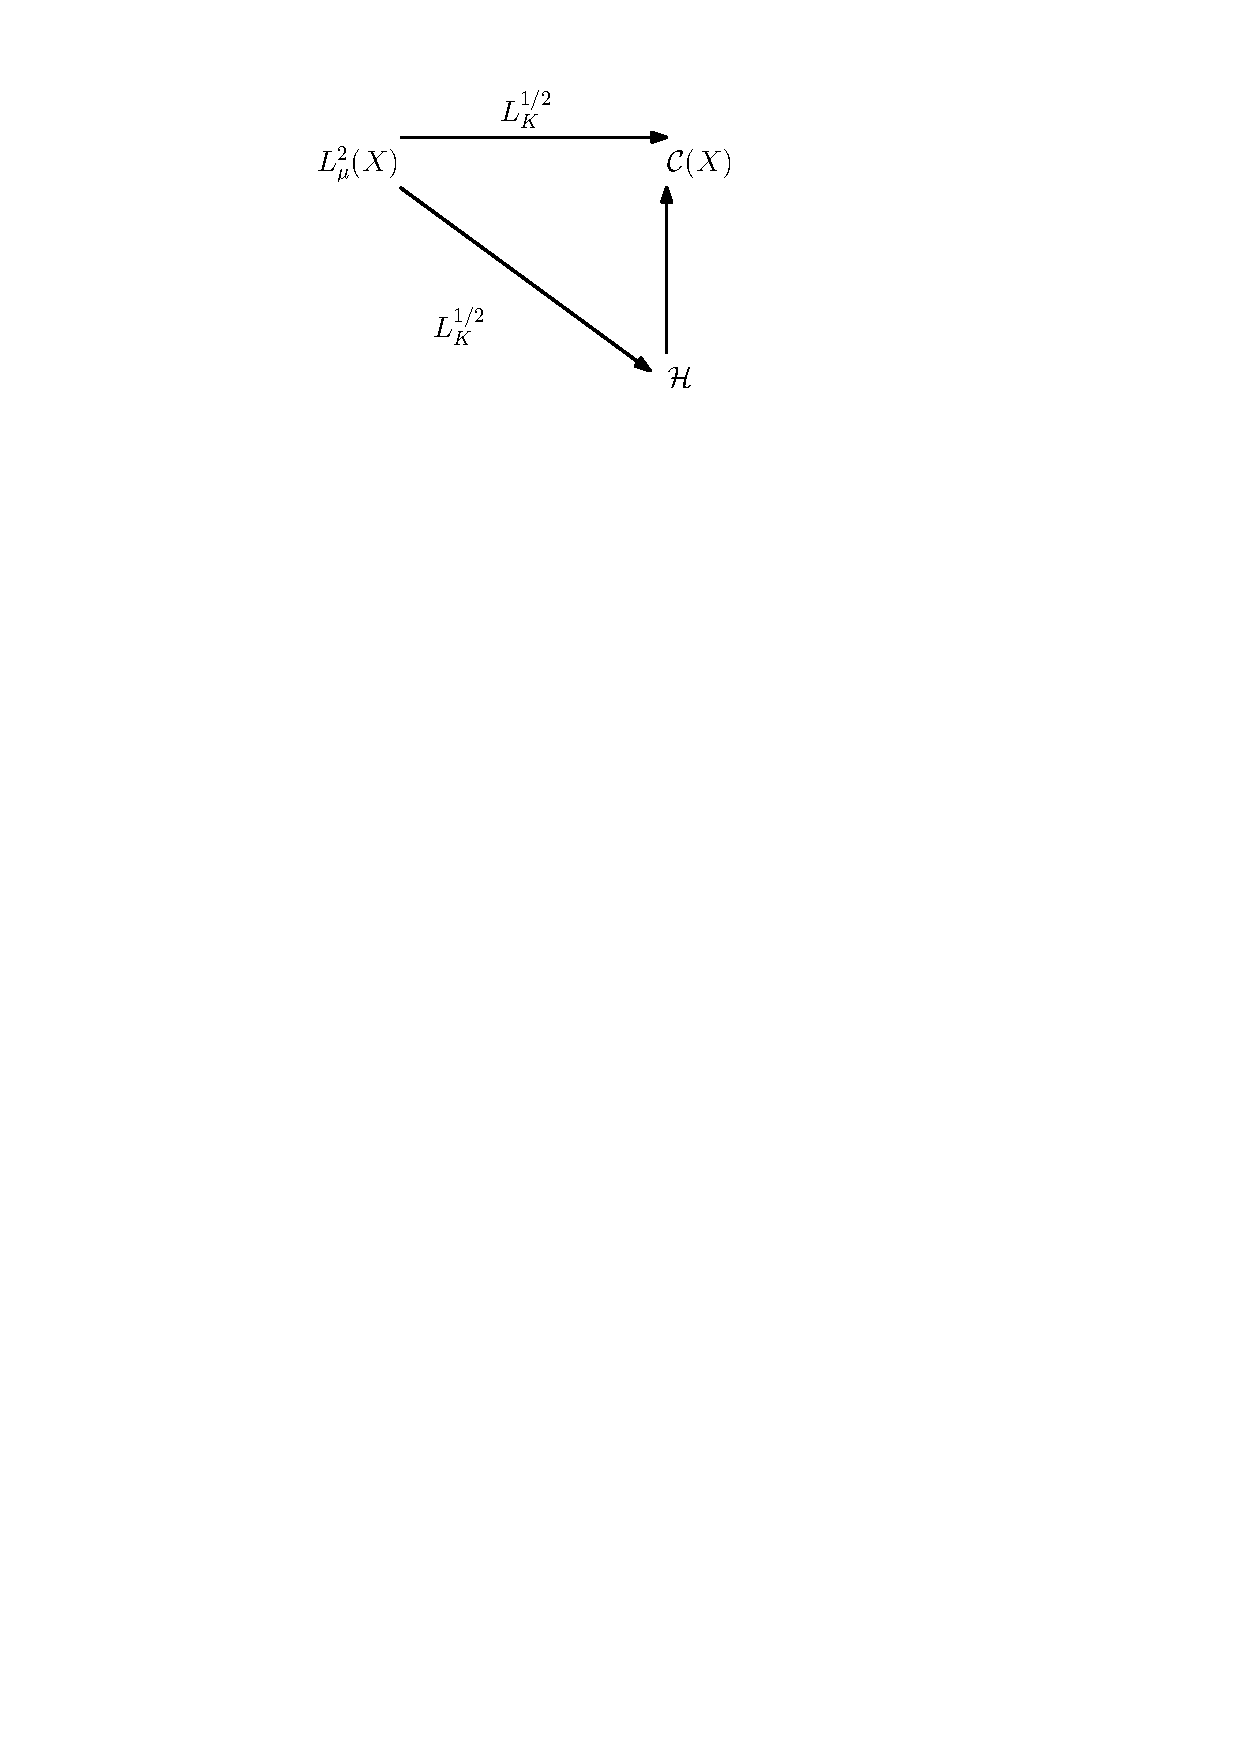
\includegraphics[width=3in]{images/Chap3_RKHS_isomorphism}
%	\caption{Diagram illustrating the isomorphic transformations between $\clH$ and $L^2_\measure$.}
%	\label{fig:rkhs_isomorphism}
%\end{figure}
%
%% $L_{K,C}$ emphasizes that the target is $\mathcal{C}(\state)$ and $I_K$ denotes the inclusion. If $\Kern$ is $\mathcal{C}^\infty$, then $I_K$ is compact. \anand{Gaussian kernel is $\mathcal{C}^\infty$}
% $L_K$ is a self-adjoint, compact operator with eigenvalues $\reg_1 \geq \reg_2 \geq \cdots \geq 0$, with the corresponding normalized eigenfunctions $\{\phi_n\}_{n=1}^\infty$ forming an orthonormal basis for $L^2_\measure(\state)$. Mercer's theorem states that 
%\begin{equation}
%\Kern(x,x') = \sum_{n=1}^\infty \reg_n \phi_n(x) \phi_n(x'),
%\end{equation}
%where the series converges absolutely for each $x,x' \in \state$. The set $\{\sqrt{\reg_n}\phi_n\}_{n=1}^\infty$ forms an orthonormal basis for $\clH$. However, finding an eigenfunction feature representation for a kernel is challenging, except in special cases. 

%\section{Properties of the Gaussian Kernel -  RKHS}
%\label{s:gaussian_rkhs}
%
%Of the many kernels being used, Gaussian kernel is the most widely used and often gives the best performance \cite{min10}. The study of the properties of the Gaussan kernel has received a lot of attention \cite{stehussco06, min10,micchaxuzha06}. The Gaussian kernel is a translation-invariant kernel given by,
%\begin{equation}
%\Kern_{\epsilon}(x,x') := \exp(-\|x - x'\|^2/ 4\epsilon) \qquad \forall x,x' \in \state,
%\end{equation}
%where $\epsilon$ is a parameter that defines the width of the kernel. An illustration of the Gaussian kernel for $\epsilon = 0.125$ and the corresponding Fourier transform is given in \Fig{fig:gaussian_kernel}. It may be seen that the Fourier transform decays exponentially fast for large values of $\omega$. The lack of high frequency components in the Gaussian kernel indicates that the functions belonging to the induced RKHS are smooth.  
%\begin{figure}[htbp]
%	\centering
%	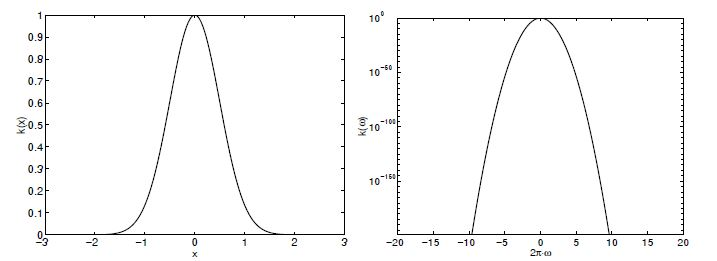
\includegraphics[width=6in]{images/Chap3_Gaussian_kernel}
%	\caption{Gaussian kernel with $\epsilon = 0.125$ and its Fourier transform \cite{schsmo01}.}
%	\label{fig:gaussian_kernel}
%\end{figure}
%
%Steinwart et al. in \cite{stehussco06} tries to answer questions like - which functions are contained in the RKHS induced by the Gaussian kernel, how the corresponding norms can be computed, and how the RKHS of different widths correlate to each other. 
%In particular, RKHS of Gaussian kernels always have countable orthonormal bases. Theorem 3 of the paper gives the orthonormal basis functions for $\clH$ defined by the Gaussian kernel $\Kern_\epsilon$. It states that for $\epsilon >0$ and $n \in \mathbb{N}_0 := \mathbb{N} \cup \{0\}$, the sequence of functions $\{\phi_n : \Re \to \Re\}$ defined by,
%\begin{equation}
%\phi_n(x) := \sqrt{\frac{1}{(2\epsilon)^n n!}}x^n \exp(-x^2/4\epsilon).
%\end{equation}
%is an orthonormal basis for $\clH$.
%
%Minh in \cite{min10} gives several properties of the RKHS induced by Gaussian kernels. Theorem 1 of the paper states that the RKHS $\clH$ induced by the standard Gaussian kernel is infinite dimensional, i.e. dim($\clH$) = $\infty$ and 
%\begin{equation}
%\clH := \Bigl\{ f = \exp(-x^2/4\epsilon) \sum_{n=0}^\infty w_n x^n: \|f\|^2_\clH = \sum_{k=0}^\infty (2\epsilon)^k k! \sum_{n=0}^k w_n^2 <\infty \Bigr\}
%\end{equation}
%Some of the salient properties of the Gaussian kernel RKHS are summarized below: 
%\begin{enumerate}
%	\item $\clH$ induced by the standard Gaussian kernel does not contain any polynomial on $\state$, including the non-zero constant function. 
%	
%	\item If $\state$ is compact, $\clH$ induced by the Gaussian kernel is dense in the space of $\mathcal{C}(\state)$ of continuous functions on $\state$.
%	This means that given a continuous function $h(x)$, for all $\varepsilon >0$, we can find a function $g(x) \in \clH$ such that 
%	\begin{equation}
%	\|h(x) - g(x)\|_\infty \leq \epsilon \qquad \forall x \in \state
%	\end{equation} 
%	\item Let $\Kern_{\epsilon}(x,x') = \exp(-\frac{\|x-x'\|^2}{4\epsilon})$. The Hilbert space $\clH_\epsilon$ induced by $\Kern_\epsilon$ on $\state$ contains the function $\exp(-\frac{c \|x\|^2} {4 \epsilon})$ if and only if $0<c <2$. For example, $\exp(-\frac{\|x\|^2}{2 \epsilon}) \in \clH_{\epsilon/2}$, but  $\exp(-\frac{\|x\|^2}{2 \epsilon}) \notin \clH_{\epsilon}$. As $c=0$ is excluded, it validates the first property that constant functions do not belong to $\clH$.
%	
%	\item The functions in $\clH$ that are smooth are not necessarily integrable, as $\clH \notin L^1(\Re^n)$ for any $\epsilon >0$.  This implies that $L^1$ norm optimization or regularization is infeasible in $\clH$. This could still be done on subsets of finite linear combinations of the basis functions.
%	
%
%\item Partial derivatives of the Gaussian kernel denoted as $\frac{\partial^n}{\partial x^n} \Kern_x \in \clH$. As a corollary, it can be shown that $t^n \Kern_x(t)\in\clH$. Additionally, for any polynomial $p(t)$, $p(t) \Kern_x(t) \in \clH$. An expression for the Hilbert space norm for kernel derivative of any order $d$ is also provided in \cite{min10}. 
%\end{enumerate}
%
%The paper by Michelli et al. \cite{micchaxuzha06} sets out to identify kernels with universal approximating property, i.e. given any compact set $\state$, any function $f \in \mathcal{C}(\state)$, there is a function $g \in \clH$ such that $\| f - g\|_{\infty} \leq \varepsilon$ holds for any $\varepsilon > 0$. Thus for any choice of compact set $\state$, the space $\clH$ is dense in $\mathcal{C}(\state)$ in the maximum norm. A kernel that satisfies this property is called the universal kernel. The paper discusses the characterization of universal kernels in terms of feature map representation of the kernel $\Kern$. It provides necessary and sufficient condition for $\Kern$ to have the universal approximation property in terms of its features. Under conditions provided in Theorem 17 of the paper, the standard Gaussian kernel is shown to be universal. 

% The below section needs to go in Chapter 4 on FPF

\subsection{Examples of reproducing kernel functions}
It is evident from the construction of the RKHS that the properties of the functions in $\clH$ are governed by the properties of its kernel $\Kern$. Therefore, by choosing different kernel functions, different function spaces can be generated. Typically, $\Kern$ depends on a variable hyperparameter, which can be tuned to control the scaling. Some commonly used kernel functions are:
\begin{arabnum}
\item Linear kernel: The simplest example is a linear kernel in one dimension:
\begin{equation}
\Kern(x,x') \eqdef x x', \qquad x,x' \in \state.
\end{equation}
\item Polynomial kernel: It has been shown by Aronszajn \cite{aro50} that sums and products of kernel functions are also kernels. Polynomial kernels are obtained by taking combinations of linear kernels:
\begin{equation}
\Kern(x,x') = (xx' + a)^b, \qquad x,x'\in \state, a \in \Re, b \in \mathbb{N}.
\end{equation}
\item Radial basis function kernels: Both linear and polynomial kernels depend on the absolute location of the inputs. Radial basis functions are a class of kernels that are translation-invariant, i.e. their values only depend on the relative positions of the inputs, and not the absolute values themselves. They are essentially a measure of similarity, in the sense that the proximity of the points in the input space determines the value of the kernel. A class of radial basis function kernels may be defined as:
\begin{equation}
\Kern(x,x') \eqdef g(\gamma_1, \|x-x'\|^{\gamma_2})
\end{equation}  
The most popular example of a radial basis kernel is the exponential kernel defined as $\Kern(x,x') \eqdef \exp(-\gamma_1 \|x - x'\|^{\gamma_2})$, of which the standard Gaussian kernel is a special case:
\[
\Kern_\epsilon \eqdef \exp\Bigl\{\frac{\|x-x'\|^2}{4 \epsilon}\Bigr\},
\]
where $\epsilon$ is the variance parameter that controls the width of the function. Desirable properties of the Gaussian kernel that makes it widely used have been investigated in \cite{min10,stehussco06}. A brief review is provided in \Appendix{a:gaussian_rkhs}. 
\end{arabnum}

More composite kernel functions can be constructed by taking various combinations of reproducing kernels. 
\section{Empirical Risk Minimization (ERM)}
\label{s:erm}
In this dissertation, kernel methods and RKHS are employed with the ultimate objective of acting as an approximating function space to be used in the $\gradTD$ learning algorithms presented in \Chapter{ch:diff_td}. As mentioned earlier, RKHS has a rich history of being used for learning functions from observed data. Such class of problems termed empirical risk minimization (ERM) have been well studied in statistical learning theory literature. In order to utilize the RKHS theory, the $L^2(\pr)$ norm-minimization problem in \eqref{e:gradTD_norm_error} needs to be fit in an ERM framework. In this section, a primer on ERM is provided, followed by the necessary transformations that lead to an ERM formulation for the $\gradTD$ learning problem.  

In an ideal setting, the goal of a learning problem is to find an approximation of a function $f_\pr : \state \to Y$, when only a pair of values $\bm{z} = (x_i, y_i)_{i=1}^N$ drawn from an unknown probability measure $\pr$ on $\state \times Y$ is available. Usually, $\state$ is a compact domain and $Y = \Re$. For a least-squares regression problem, the best target function often called the regression function is the minimizer of:
\begin{equation}
f_\pr \eqdef \argmin_f \int_{\state \times Y} (f(x) - y) ^2 d\pr,
\label{e:least_sq_regression}
\end{equation}
it takes the form:
\begin{equation}
f_\pr(x) = \int_Y y d\pr(y|x).
\label{e:f_rho}
\end{equation}
In practice, it is not possible to obtain $f_\pr$ due to two reasons. First, $\pr$ is unknown and only a finite number of sample points are available for estimation and therefore, it is not possible to carry out the integration \eqref{e:f_rho}. Secondly, since the approximating function space that is chosen is typically a small subspace, an exact match for $f_\pr$ may not be obtained within this space. Hence, we focus on minimizing the empirical risk on observed data:
\begin{equation}
f_{\bm{z}} \eqdef \argmin_f \frac{1}{N} \sum_{i=1}^N (y_i - f(x_i))^2.
\label{e:erm}
\end{equation}
Assuming, $N$ is large enough and $\bm{z} \sim \pr$, \eqref{e:erm} can be thought of as approximating \eqref{e:least_sq_regression} quite well.   In a non-parametric setting, this problem is ill-posed and can have infinitely many solutions. This is resolved by adding an extra regularization term to the objective function. 
A common approach followed is to minimize,
\begin{equation}
f_{\bm{z},\reg} := \argmin_f \frac{1}{N}\sum_{i=1}^N (y_i - f(x_i))^2 + \reg \|A f \|^2_{\mathcal{L}_{\pr}^2(\state)},
\label{e:erm_regularized}
\end{equation}
where $A$ is an operator and $\mathcal{L}^2_{\pr}(\state)$ is the Hilbert space of square integrable functions on $\state$ with measure $\pr_\state$ on $\state$ and $\reg>0$ is the regularization parameter. 
The key objective in an ERM problem is not just to obtain a good fit on the observed data, but to generalize well on ``unseen'' data as well. If the standard $L^2$ norm is used for regularization, \eqref{e:erm_regularized} is called the ridge regression. To obtain sparse solutions, $L^1$-regularization is used, which forms the LASSO technique. Regularization is used to prevent overfitting and achieve better generalization.   In this dissertation, we consider a Tikhonov regularization scheme \cite{tikars79} associated with Mercer kernels.
\anand{ridge and LASSO needs citations}

\subsection{ERM in an RKHS setting}
\label{s:erm_rkhs}
Now that the utility of regularized empirical risk minimization has been motivated, we consider a more general formulation of an ERM in an RKHS setting. A loss function $L \colon  \state\times \Re \to\Re$ is given. It is not necessary that the loss function takes the mean-squared error form in \eqref{e:erm_regularized}. Given an RKHS $\clH$, the goal is to find the function $f_\reg^*\in\clH$ that solves the infinite-dimensional regularized optimization problem:
\begin{equation}
f_\reg^* \eqdef \argmin_{f\in\clH} \underbrace{\frac{1}{N} \sum_{i=1}^N L(y_i,  f(x_i))}_{\text{Empirical risk}}    + \underbrace{\Omega(\| f\|_{\clH})}_{\text{Regularization}}.
\label{e:erm_rkhs}
\end{equation}
The objective function in \eqref{e:erm_rkhs} consists of an empirical risk term, that minimizes the error on observed data, and a regularization term that controls the properties of the model. It is important to note that the regularization term is independent of the observed data sequence $\bf{z}$. The function $\Omega : [0, \infty] \to \Re$ is strictly monotonically increasing. Often, $\Omega$ is chosen to be proportional to a quadratic function of the norm $\|\cdot\|_\clH$, such as $\reg \|f\|^2_\clH$.  The value of the regularization parameter $\reg$ controls the trade-off between the empirical error term and the smoothness of the estimated function. In other words, a larger value for $\reg$ reduces the variance of the estimates by reducing its dependency on $\bf{z}$, but at the cost of introducing bias to the model. Regularization is necessary to ensure the well-posedness of the problem and increasing $\reg$ improves the numerical stability of the algorithm. 
\anand{A few words about ways to choose the best $\lambda$.}

The remarkable theme in the RKHS literature is that while the optimization problem in \eqref{e:erm_rkhs} is infinite dimensional,  the optimizer lies in an identifiable finite-dimensional subspace.
The result is due to the classical version of the representer theorem of Kimeldorf and Wahba \cite{kimwah71}. The original form of the theorem considered the mean-squared loss $L(y_i, f(x_i)) = (y_i - f(x_i))^2$. An extension to non-quadratic loss functions was provided in \cite{coxsull90}. The classical version of the representer theorem is stated next and its proof presented in \cite{schhersmo01} is provided in \Appendix{a:rep_theorem}. 
\begin{theorem}[Representer Theorem]
\label{theorem:rep_theorem}
The minimizer $f_\reg^* \in \clH$ of the regularized risk \eqref{e:erm_rkhs} for an arbitrary loss function $L(y_i, f(x_i))$ lies in the span of kernel functions centered at the sample points, $\Kern(x_i, \cdot)$,
\[
f_\reg^*(x) = \sum_{i=1}^N \rkhsparam_i \Kern(x_i, x)
\]
\qed
\end{theorem}
%\begin{proof}
%From the definition of the RKHS $\clH$, any $f$ of the form:
%\[
%f \eqdef \sum_{i=1}^N  
%\rkhsparam_i \Kern(x_i,\cdot),
%\]
%is in $\clH$. 	
%Denote the linear subspace of $\clH$ made up of all such functions $f$ that are finite linear combinations of the kernel functions centered at $x_i$,
%\[
%\clH_\parallel := \Bigl\{f \in \clH\, |\, f = \sum_{i=1}^N  \rkhsparam_i \Kern(x_i,\cdot) \Bigr\},
%\]
%where $N$ ranges over $\mathbb{Z}_+$, and  each $\rkhsparam_i \in \Re$ for each $i$. Denote by $\clH_{\perp}$, the subspace of $\clH$ orthogonal to $\clH_\parallel$:
%\[
%\clH_\perp : = \{ \tilf \in \clH\,| \, \langle \tilf , f \rangle_\clH = 0 ,\, \forall f \in \clH_\parallel \}
%\]
%We can see that every $f \in \clH$ can be uniquely decomposed into a component lying within $\clH_\parallel$, denoted by $f_\parallel$ and a component lying within $\clH_\perp$, denoted by $f_\perp$.
%The $\clH$-norm can be written as,
%\[
%\Omega(\|f\|_\clH) = \Omega( \|f_\parallel + f_\perp\|_\clH) =\Omega( \sqrt{\|f_\parallel\|^2_\clH + \|f_\perp\|^2_\clH})  \geq \Omega(\|f_\parallel\|_\clH)
%\]
%This implies that the regularization term in \eqref{e:erm_rkhs} is minimized if $f$ lies in the subspace $\clH_\parallel$.
%Additionally, using reproducing property of the kernel $\Kern$,
%\[
%\begin{aligned}
%f(x_i) & =  \langle f \, , \Kern(x_i,.) \rangle_\clH\\
%&  = \langle f_\parallel\, , \Kern(x_i,.) \rangle_\clH + \langle f_\perp \, , \Kern(x_i,.) \rangle_\clH \\
%&  = \langle f_\parallel\, , K(x_i,.) \rangle_\clH \\
%&  = f_\parallel(x_i).
%\end{aligned}
%\]
%Therefore,
%\[
%L(x_i, f(x_i)) = L(x_i, f_\parallel(x_i))
%\]
%The empirical error term depends only on the component $f_\parallel$. Hence, the regularized objective function is minimized if $f_\reg^*$ lies within $\clH_\parallel$ and takes the form,
%\[
%f^*(x) = \sum_{i=1}^N  \rkhsparam_i^*  \Kern(x_i, x)
%\]
%This concludes the proof. 
%\end{proof}
Sch\"{o}lkopf et al. in \cite{schhersmo01} present two more generalized versions of the representer theorem, called the semiparametric representer theorem and biased regularization. Semiparametric representer theorem is particularly useful as it allows a combination of finitely parameterized family of functions and an RKHS to be used as the approximating function space. The proof for this extension is straight forward.  

\begin{theorem}[Semiparametric Representer Theorem]
In addition to assumptions in \Theorem{theorem:rep_theorem}, if a set of $M$ real-valued functions $\{\psi_j\}_{j=1}^M : \state \to \Re$ is given, with the property that they are linearly independent, then any $\tilf \eqdef f + g$, where $f \in \clH$ and $g \in$ span $\{\psi_j\}$, then the minimizer of the regularized risk functional,
\begin{equation*}
\tilf^*_\reg(x) \eqdef \argmin_{\tilf} \frac{1}{N} \sum_{i=1}^N L(y_i,\tilf(x_i)) + \Omega(\|f\|_\clH)
\end{equation*}
admits a representation of the form
\begin{equation*}
\tilf(x) = \sum_{i=1}^N \rkhsparam_i \Kern(x_i, x) + \sum_{j=1}^M \gamma_j \psi_j(x)
\end{equation*}
with $\gamma_j \in \Re$ for all $j \leq M$. 
\end{theorem}
\anand{Read spline smoothing problem in Bhujwalla's thesis and see if this can be applied for gradient regularization.} 
\section{Kernel Methods for Differential TD-Learning}
\label{s:kernel_choices}

In this Section, the goal is to construct an ERM problem in an RKHS setting, such that it closely approximates the objective function in the $\gradTD$ learning algorithm \eqref{e:gradTD_norm_error}. The loss function $L$ will be chosen so that the optimizing function approximately solves \eqref{e:gradTD_norm_error_infinite}; the infinite dimensional variant of \eqref{e:gradTD_norm_error}. 
\begin{equation}
\| \nabla h -  \nabla g \|^2_{L^2}   \eqdef \sum_{k=1}^d    \Bigl\|  \frac{\partial}{\partial x_k} (h-g)  \Bigr\|^2_{L^2}
\, .
\label{e:gradTD_norm_error_infinite}
\end{equation}
The fact that the original objective function aims to minimize the approximation error in $L^2(\pr)$ norm helps in the construction of an equivalent ERM.

Candidates for the loss function $L$ are discussed here: 
If the values $\{x_i\} \subset \state $  are sampled randomly and independently according to $\pr$,  then by the law of large numbers, for large $N$,
\begin{equation}
\frac{1}{N} \sum_{i=1}^N L(x_i, g(x_i), \nabla g\, (x_i))  \approx
\int  L(x, g(x), \nabla g\, (x))  \pr(x)\, \ud x.
\end{equation}
The independence assumption is not essential; the samples $\{x_i\}$ may very well be generated by an ergodic Markov chain with $\pr$ as its invariant density. 

In view of \eqref{e:gradTD_norm_error_infinite}, the ideal loss function is thus
\begin{equation}
L^*(x,g(x) ,\nabla g \,(x))  =         \| \nabla h\,(x)  -\nabla g\, (x) \|^2\,, \quad x\in\state\,.
\label{e:IdealLoss}
\end{equation}
The difficulty with this definition is that $L^*$ in its current form is not computable as $\nabla h$ is unknown. This is resolved by applying the special structure of the differential generator $\generate$,  stated in \Prop{prop:lang_generator_grad}:
\begin{proposition}
	\label{prop:gradTD_erm_loss}
	If $h$ is a solution to Poisson's equation satisfying $h\in C^2\cap L^2$, then
	\[
	\| \nabla h -  \nabla g\|^2_{L^2} =\| \nabla h  \|^2_{L^2} + \int   L^\bullet(x, g(x), \nabla g\, (x)) \pr(x)\, \ud x
	\]
	where
	$ L^\bullet(x, g(x), \nabla g\, (x)) =   \| \nabla g(x)\|^2   - 2 \tilc(x) g(x)$.
	\qed
\end{proposition}
\proofAlt{Proof of \Prop{prop:gradTD_erm_loss}}
Expanding $L^*$ gives,	
\[
\begin{aligned}
L^*(x,g(x),\nabla g(x)) & = \| \nabla h(x) - \nabla g(x) \|^2 \\
& = \| \nabla h(x) \|^2 + \| \nabla g(x) \|^2- 2 \nabla h(x) \cdot \nabla g(x) \\
\end{aligned}
\]
To establish the proposition, it remains to show that,
\[
\int \nabla h(x) \cdot \nabla g(x) \pr(x) \ud x = \int \tilc(x) g(x) \pr(x) \ud x.
\label{e:transform}
\]
This follows from an application of \Prop{prop:lang_generator_grad}:
\[
\begin{aligned}
\langle \nabla h, \nabla g \rangle_{L^2} & \eqdef \int \nabla h(x) \cdot \nabla g(x) \pr(x) dx \\
& = - \int  (\generate h(x)) g(x) \pr(x) dx \\
& = \int \tilc(x) g(x) \pr(x) dx \qquad & \text{(from \eqref{e:poissons})}
\end{aligned}
\]
\qed
\Prop{prop:gradTD_erm_loss} motivates the ERM introduced in this dissertation:	
\begin{equation}
g^*  := \argmin_{g \in \clH} \frac{1}{N} \sum_{i=1}^N\Bigl[ \underbrace{\| \nabla g(x_i) \|^2 - 2 \tilc_N(x_i)g(x_i)}_{L^\bullet (x_i, g(x_i), \nabla g(x_i))}\Bigr] + \lambda \|g\|^2_\clH
\label{e:erm_diff_td}
\end{equation}
in which the centered function $\tilc$ is also approximated:
\[
\tilc_N(x) = c(x) - \frac{1}{N}  \sum_{i=1}^N  c(x_i)\,,\quad x\in\state\, .
\label{e:tilc_N}
\]
The term $\| \nabla h \|^2$ can be conveniently dropped from \eqref{e:erm_diff_td} as it does not affect the optimization problem.

\subsection{Extended representer theorem}
It may be seen that the ERM in \eqref{e:erm_diff_td} falls in the standard form in \eqref{e:erm_rkhs} except that the loss function $L^\bullet$ depends on the gradient of the estimator $g$. Problems of this form where learning with gradients is required The classical version of the representer theorem (\Theorem{theorem:rep_theorem}) is valid under the assumption that the loss function $L$ depends only on $g$. In this dissertation, as we are interested in loss functions of the form 
\begin{equation}
\min_{g\in\clH} \Bigl\{  \frac{1}{N} \sum_{i=1}^N L(x_i,  g(x_i), \nabla g\, (x_i))     + \lambda \| g\|^2_{\clH}  \Bigr\},
\label{e:erm_rkhs_gradient}
\end{equation}
where the function $L$ includes $\nabla g$, it cannot be applied directly. The extension to include differential loss (including gradient terms) appeared in \cite{zho08}. The main motivation in this work is to extend the RKHS theory to applications that may have gradient data or unlabeled data available for improving learning ability. Two types of problems are presented - one in which the loss function includes a term with gradients of the estimator function evaluated at the unlabeled points, called semi-supervised learning and a second where, gradient values at sample points are available and the algorithm is required to learn the function values and the gradients simultaneously, called the Hermite learning algorithm. Potential applications discussed are in image processing, where gradient fitting is used to preserve edges and discontinuities and avoiding staircasing effects \cite{didsetste09}. 
 
Similar to the standard representer theorem, that guarantees a finite dimensional solution to a potentially infinite dimensional ERM problem, an extended version is presented in \cite{zho08} that can be applied to cases where the loss functions include partial derivatives of the estimator. This version is stated here followed by its proof. 
\begin{theorem}[Extended Representer Theorem]
	\label{theorem:ext_rep_theorem}
	Suppose that $L(x, g(x),\nabla g)$ is a convex function on $\Re^{d+1}$ for each $x\in\state$.
	Then the  optimizer $g^*$ of \eqref{e:erm_rkhs_gradient} over $g\in\clH$ exists, is unique, and has the following representation: \anand{change $x_k$ to $x^k$}
	\[
	g^*(x) = \sum_{i=1}^N  \Bigl[
	\rkhsparam_i^{0*}  K(x_i,x)   +  \sum_{k =1}^d  \rkhsparam_i^{k*} \frac{\partial K}{\partial x_k} (x_i, x) \Bigr],
	\]
	where $\{\rkhsparam_i^{k*} \colon i=1,\cdots,N,\, k = 0,\cdots,d\}$ are real numbers.
	\qed
\end{theorem}
\begin{proof}
 The proof provided here is a special case of the proof for a more general version of the extended representer theorem appearing in \cite{zho08}. The partial derivative reproducing property of the kernel $\Kern$ stated and proved in \cite[Theorem 1]{zho08}, presented as \Lemma{lemma:der_rep_property} is used in the proof.  
 \begin{lemma}
 If $\Kern :\state \times \state \to \Re$ is a Mercer kernel such that $\Kern \in C^2$, then the following statements hold:
 \begin{romannum}
 \item For any $x \in \state$, $\frac{\partial \Kern}{\partial x_k} \in \clH$. 
 \item A partial derivative reproducing property holds:
 \begin{equation}
 \frac{\partial f(x)}{\partial x_k} = \Bigl \langle \frac{\partial K(x, \cdot)}{\partial x_k} , f(\cdot) \Bigr \rangle_\clH \qquad \forall x \in \state, \forall f \in \clH.
 \end{equation}
 \end{romannum}
 \label{lemma:der_rep_property}
 \end{lemma}
 By \Lemma{lemma:der_rep_property}, $\frac{\partial K}{\partial x_k}(x_i,.) \in \clH$ for each $k$.
Therefore, any $f$ of the form:
	\[
	f \eqdef  \sum_{i=1}^N  \Bigl[
	\rkhsparam_i^{0}  K(x_i, .)   +  \sum_{k =1}^d  \rkhsparam_i^{k} \frac{\partial K}{\partial x_k}  (x_i, .) \Bigr],
	\]
	is in $\clH$. The rest of the proof proceeds using arguments similar to those in the proof of \Theorem{theorem:rep_theorem}. 

Let us denote by $\clH_\parallel$, the linear subspace of $\clH$ made up of all such functions $f$,
	\[
	\clH_\parallel := \Bigl\{f \in \clH\, |\, f = \sum_{i=1}^N \Bigl[ \rkhsparam^0_i K(x_i,.) + \sum_{k=1}^d \rkhsparam_i^k \frac{\partial K }{\partial x_k} (x_i, .)\Bigr]\Bigr\},
	\]
	where $N$ ranges over $\mathbb{Z}_+$, and  each $\rkhsparam_i^k \in \Re$ for each $i$ and $k = 0$ to $d$. Let $\clH_{\perp}$ be the subspace of $\clH$ orthogonal to $\clH_\parallel$:
	\[
	\clH_\perp : = \{ \tilf \in \clH\,| \, \langle \tilf , f \rangle_\clH = 0 ,\, \forall f \in \clH_\parallel \}
	\]
	We can see that every $g \in \clH$ can be uniquely decomposed into a component lying within $\clH_\parallel$, denoted by $g_\parallel$ and a component lying within $\clH_\perp$, denoted by $g_\perp$.
	The $\clH$-norm can be written as,
	\begin{equation}
	\|g\|^2_\clH = \|g_\parallel + g_\perp\|^2_\clH = \|g_\parallel\|^2_\clH + \|g_\perp\|^2_\clH \geq \|g_\parallel\|^2
	\label{e:g_reg}
	\end{equation}
	This again implies that the regularization term in \eqref{e:erm_rkhs_gradient} is minimized if $g$ lies in the subspace $\clH_\parallel$. Furthermore, using the reproducing property of the kernel $K$,
	\begin{equation}
	\begin{aligned}
	g(x_i) & =  \langle g \, , K(x_i,.) \rangle_\clH\\
	&  = \langle g_\parallel\, , K(x_i,.) \rangle_\clH + \langle g_\perp \, , K(x_i,.) \rangle_\clH \\
	&  = \langle g_\parallel\, , K(x_i,.) \rangle_\clH \\
	&  = g_\parallel(x_i),
	\end{aligned}
	\label{e:g_parallel}
	\end{equation}
	and partial derivative reproducing property, we have for all $k = 1, \cdots, d$,
	\begin{equation}
	\begin{aligned}
	\frac{\partial g(x_i)}{\partial x_k} & = \Bigl \langle g \, , \frac{\partial K}{\partial x_k} (x_i,.) \Bigr \rangle_\clH\\
	&  = \Bigl \langle g_\parallel\, , \frac{\partial K}{\partial x_k} (x_i,.)  \Bigr \rangle_\clH + \Bigl \langle g_\perp \, ,\frac{\partial K}{\partial x_k} (x_i,.) \Bigr \rangle_\clH \\
	&  = \langle g_\parallel\, , \frac{\partial K}{\partial x_k} (x_i,.) \rangle_\clH \\
	&  = \frac{\partial g_\parallel(x_i) }{\partial x_k}.
	\end{aligned}
	\label{e:der_g_parallel}
	\end{equation}
	From \cref{e:g_parallel,e:der_g_parallel}, it is clear that the empirical error term depends only on the component $g_\parallel$,
	\[
	L(x_i, g(x_i),\nabla g(x_i)) = L(x_i, g_\parallel(x_i),\nabla g_\parallel(x_i)),
	\]
	and from \eqref{e:g_reg}, $g_\parallel$ minimizes the regularization term. Hence, the regularized objective function is minimized if $g^*$ lies within $\clH_\parallel$ and takes the form,
	\[
	g^*(y) = \sum_{i=1}^N  \Bigl[ \rkhsparam_i^{0*}  K(x_i, y)   +  \sum_{k =1}^d  \rkhsparam_i^{k*} \frac{\partial}{\partial x_k}  K(x_i, y) \Bigr]
	\]
\end{proof}

\subsection{Optimal solution in one dimensional case}
\label{sec:one_dimension}
We first provide a full description of the solution to \eqref{e:erm_diff_td} for the one-dimensional model in this section. The optimizer is obtained as the solution to a system of linear equations, extensions to higher dimensions is straight-forward and provided towards the end of the section. 
The regularized ERM problem \eqref{e:erm_diff_td} in one-dimension reduces to the following:
\begin{equation}
g^* := \argmin_{g\in\clH} \frac{1}{N} \sum_{i=1}^N \Bigl\{ (g'(x_i))^2 - 2 \tilc_N(x_i) g(x_i) \Bigr\} + \lambda \|g\|^2_\clH,
\label{e:1dloss}
\end{equation}
where $g' = d g / d x$. Using the extended form of the Representer Theorem (\Theorem{theorem:ext_rep_theorem}), the optimizer $g^*$ has the following form:
\begin{equation}
g_\rkhsparam(y)= \sum_{i=1}^N \Bigl[\rkhsparam_i^{0} K(x_i,y) + \rkhsparam_i^{1} \frac{\partial K}{\partial x}(x_i,y)\Bigr], \qquad y \in \state
\label{e:g_star}
\end{equation}
\Theorem{theorem:ext_rep_theorem}  states that the solution to  the infinite dimensional optimization problem reduces to a quadratic program over $\Re^{2N}$ when there are $N$ samples. A formula for the optimizer  $\rkhsparam^* \in \Re^{2N}$ is obtained as follows.
%\[
% \begin{aligned}
% \rkhsparam^* & = \argmin_{\rkhsparam \in \Re^{2N}} &\frac{1}{N}  \sum_{j=1}^N \left( \sum_{i=1}^N \Bigl[ \rkhsparam_i^0 \frac{\partial K}{\partial y}(x_i,x_j)  +  \rkhsparam_i^1 \frac{\partial^2 K}{\partial x \partial y}(x_i,x_j)\Bigr] \right)^2 -	\frac{1}{N} \sum_{j=1}^N 2 \tilc(x_j) \left(\sum_{i=1}^N \Bigl[\rkhsparam_i^0 K(x_i,x_j) + \rkhsparam_i^1 \frac{\partial K}{\partial x}(x_i,x_j)\Bigr] \right)  + \\
% &  & \lambda \sum_{j=1}^N \sum_{i=1}^N \Bigl[ \rkhsparam_i^0 \rkhsparam_j^0 K(x_i,x_j) \, + \, \rkhsparam_i^0 \rkhsparam_j^1 \frac{\partial K}{ \partial x} (x_j,x_i) + \rkhsparam_i^1 \rkhsparam_j^0 \frac{\partial K}{\partial x} (x_i,x_j) \, + \, \rkhsparam_i^1 \rkhsparam_j^1 \frac{\partial^2 K}{\partial x \partial y}(x_i, x_j) \Bigr] \\
% \end{aligned}
% \label{e:beta}
% \]
Introduce vectorized notation:
\[
\boldsymbol{\rkhsparam}^\transpose   := [\rkhsparam_1^0 ,\dots,  \rkhsparam_N^0 \,,\, \rkhsparam_1^1 ,\dots,  \rkhsparam_N^1],  \quad  \boldsymbol{\zeta}^\transpose  := [\tilc_N(x^1) ,\dots, \tilc_N(x^N)],
\]
and introduce matrices $M_{00}, M_{10}, M_{01}, M_{11}$,  whose   $\{i,j\}^{th}$ entries are defined as follows:
\[
\begin{aligned}
M_{00}(i,j) &:= K(x_i,x_j)
\quad
& M_{10}(i,j) &:= \frac{\partial K}{\partial x}(x_i,x_j)
\\
M_{01}(i,j) &:= \frac{\partial K}{\partial y}(x_i,x_j)
\quad
& M_{11}(i,j) &:= \frac{\partial^2 K}{\partial x \partial y}(x_i,x_j).
\end{aligned}
\]	
Here, $\frac{\partial }{\partial x}$ and $\frac{\partial}{\partial y}$ refer to the partial derivatives with respect to the first variable and second variable of $\Kern(x,y)$ respectively.
\begin{proposition}
	\label{prop:beta_star}
	The optimal parameter vector $\rkhsparam^*$ is,
	\begin{equation}
	\rkhsparam^* = M^{-1} b
	\label{e:beta_2N}
	\end{equation}
	\begin{equation*}
	\begin{aligned}
	\text{where,
	}
	\quad
	M & := \frac{1}{N} \left[\begin{array}{c} M_{01}\\ \hline M_{11} \end{array}\right] [ M_{10} \,| M_{11}] + \lambda  \left[
	\begin{array}{c|c}
	M_{00} & M_{01} \\
	\hline
	M_{10} & M_{11}
	\end{array}
	\right] \\
	b & :=  \frac{1}{N} \left[ \begin{array}{c} M_{00} \\ \hline M_{10} \end{array}\right] \boldsymbol{\zeta}
	\end{aligned}
	\label{e:beta_optimal}
	\end{equation*}
	\qed
\end{proposition}
The derivation of the optimal parameter $\rkhsparam^*$ is analogous to the derivation of the optimal $\theta^*$ in the finite basis case in \Lemma{lemma:gradTD}. The proof of \Prop{prop:beta_star} follows from elementary calculus. 

Following the above derivation, for an arbitrary dimension $d$, using the following matrix notation with $1 \leq m,n \leq d$ and $1 \leq i,j \leq N$:
\[
M_{m0}(i,j) := \frac{\partial K}{\partial x^m}(x_i,x_j),
\quad 
M_{0n}(i,j) := \frac{\partial K}{\partial y^n}(x_i,x_j),
\quad
M_{mn}(i,j) := \frac{\partial^2 K}{\partial x^m \partial y^n}(x_i,x_j).
\]	
\begin{equation*}
\begin{aligned}
\text{where,
}
\quad
M & := \frac{1}{N} \left[\begin{array}{c} M_{01} \\ \vdots \\ M_{d1} \end{array}\right] [ M_{10} \, \hdots M_{1d}] + \lambda  \left[
\begin{array}{c c c}
M_{00}  & \hdots & M_{0d}\\
\vdots & \vdots &  \vdots \\
M_{d0} & \hdots & M_{dd}
\end{array}
\right] \\
b & :=  \frac{1}{N} \left[ \begin{array}{c} M_{00} \\ \vdots \\ M_{d0} \end{array}\right] \boldsymbol{\zeta}
\end{aligned}
\label{e:beta_optimal}
\end{equation*}
Each $M_{mn} \in \Re^{N \times N}$ and therefore $M$ is a $(d+1) N \times (d+1) N$ matrix and $b$ is a $(d+1) N$ vector. The optimal parameter vector $\rkhsparam^* \eqdef [ (\rkhsparam^0_i)_{i=1}^N, (\rkhsparam^1_i)_{i=1}^N, \hdots, (\rkhsparam^d_i)_{i=1}^N] \in \Re^{(d+1) N}$ is in the same form as \eqref{e:beta_2N}. Although, $\rkhsparam^*$ is easily computable, the solution scales poorly with dimensions. 
Moreover, there are more parameters ($(d+1)N$ than there are sample points ($N$), which is usually not preferred in machine learning. This could potentially lead to overfitting and other numerical issues.   
Ideally, we prefer an algorithm that scales well with dimensions. This leads to the following two extensions:
\begin{itemize}
	\item A reduced complexity solution \eqref{e:g_circ}.
	\item A differential regularizer \eqref{e:1dloss_diff}.
\end{itemize}
\subsection{Reduced complexity solution}
\Theorem{theorem:ext_rep_theorem} states that the optimizer of the ERM with gradient terms in the loss function lies in a subspace of the RKHS $\clH$ spanned by the kernel functions ($\Kern_{x_i}$) and its partial derivatives ($\{\partial_k K_{x_i}\}_{k=1}^d$) centered at the sample points. The main source of complexity is the presence of the $d \times N$ kernel partial derivative terms of the solution . To obtain a reduced complexity solution, $g$ is restricted to a subspace of the following form:
\begin{equation}
g(y)  := \sum_{i=1}^N \rkhsparam_i K(x_i,y).
\label{e:g_circ}
\end{equation}
\begin{proposition}
	\label{t:bcirc}
	The parameter vector $\rkhsparam^\circ \in \Re^N$ that minimizes \eqref{e:1dloss}  over all functions $g$ of the form \eqref{e:g_circ} is given by,
	\begin{equation}
	\rkhsparam^\circ  := M^{\circ -1} b^\circ   \,,
	\label{e:beta_N}
	\end{equation}
	where $ M^\circ := N^{-1} M_{01} M_{10} + \lambda M_{00}$ and $ b^\circ := N^{-1} M_{00} \, \boldsymbol{\zeta} $.
	\qed
\end{proposition}
Solutions of the form \eqref{e:g_circ} are the optimal solution given by the standard representer theorem if the loss function did not have gradient terms. 
Although, \eqref{e:beta_N} is clearly a sub-optimal solution to \eqref{e:1dloss}, $\rkhsparam^\circ$  is computationally simpler to obtain than $\rkhsparam^*$ as there are only $N$ parameters to estimate. In a surprising observation, it was found that their performance is nearly the same in numerical examples using Gaussian kernels for $d \leq 5$. More details are contained in \Section{s:numerics}.

\subsection{Differential regularizer formulation}
\label{s:diffReg} 
\anand{will come back to this later}

An alternate approach is to add a regularizing term that penalizes the $\clH$-norm of the gradient $\nabla g$ rather than $g$ itself. The modified objective for the one-dimensional model becomes,
\begin{equation}
\tilg \eqdef \argmin_{g\in\clH} \frac{1}{N} \sum_{i}^N \Bigl\{ (g'(x_i))^2 - 2 \tilc_N(x_i) g(x_i)  \Bigr\} + \lambda \|g'\|_\clH^2
\label{e:1dloss_diff}
\end{equation}
This suits our objective better as $h'$ is the function for which we seek an approximation. Bhujwalla et al. in \cite{bhujlaugil} have argued that a differential regularizer term adds more flexibility to the hyperparameter selection for the kernel function without compromising the smoothness of the approximation.

Unfortunately the representer theorem is not easily adapted to obtain a finite dimensional solution to  the optimization problem \eqref{e:1dloss_diff},  even in the differential generalization of  \cite{zho08}. The method proposed in \cite{bhujlaugil} is an ``extended representer'' through the addition of an arbitrary number of kernel functions centered at newly introduced samples.

In our case, to obtain a solution we return to the original loss function \eqref{e:IdealLoss}, which in this one dimensional setting becomes $L^*(x,g,g') = [h'(x) - g'(x)]^2$.    The associated ERM is then
\begin{equation}
g^* := \argmin_{g\in\clH} \frac{1}{N} \sum_{i=1}^N [h'(x_i) - g'(x_i)]^2 + \lambda \|g'\|^2_\clH \, .
\label{e:IdealLossERM}
\end{equation}
Since this does not depend upon $g$, we can apply the classical representer theorem to conclude that there are scalars $\{\beta^*_i\}$ such that the optimal solution has the form  ${g^*}' = g_{\beta^*}$,  where
\[
{g^*}'  = \sum_{i=1}^N  \beta_i^* K(x_i,y) \,,  \qquad y \in \state \, .
\]
We cannot use the definition \eqref{e:IdealLossERM} to compute $\beta^*$ since $h$ is not known.   However,  following the Law of Large Numbers approximation arguments,   we can obtain the value of $\beta$  by substituting $g_\beta$ of this form into the right hand side  of this variant of \eqref{e:1dloss}: \notes{Law of Large Numbers needs capitalization?}
\begin{equation*}
g^* := \argmin_{g\in\clH} \frac{1}{N} \sum_{i=1}^N \Bigl\{ (g'(x_i))^2 - 2 \tilc_N(x_i) g(x_i) \Bigr\} + \lambda \|g'\|^2_\clH,
\label{e:1dlossDiff}
\end{equation*}
and then solving the quadratic optimization problem to obtain $\beta^*$.

This approach requires a kernel   for which we can easily compute
\[
K_-(x,y) = \int_{-\infty}^y  K(x,r)\,  \ud r
\]
so that
\[
g_\beta =  \sum_{i=1}^N \beta_i  K_-(x_i,\varble)
\]
It is not clear if the optimal solution has this form for dimension greater than one -- this is another topic of current research.


\section{Algorithm Design and Error Analysis}
\label{s:error_analysis}
After choosing an appropriate loss function \eqref{e:erm_diff_td} to suit our objective, the next choice in the algorithm is that of a suitable kernel function $\Kern$. In the case of $\gradTD$ learning, desirable properties of the RKHS used as the approximating function space will help us make an informed choice.   More discussion on choosing the kernel in the context of $\gradTD$ learning is reserved for \Section{s:kernel}. An equally important step in the algorithm design is the choice of kernel hyperparameters and the regularization parameter $\reg$. The importance of a good choice of $\reg$ is illustrated with examples in \cite{wah90}. Methods such as ordinary cross-validation and generalized cross-validation are suggested. As mentioned before, a large value of $\reg$ introduces bias and a small value of $\reg$ contributes to the variance of the error. A general criteria chosen to obtain the optimal $\reg^*$ is to minimize the sum of the bias and the variance terms. Also, it may be seen that a good choice of $\reg$  depends on the number of samples $N$. $\reg(N)$ is chosen to be a decaying function of $N$ such as $\propto \frac{1}{N}$ or $\frac{1}{\sqrt{N}}$. 



It is of interest to analyze the quality of the estimates obtained. A large body of literature is available that tries to obtain the error bounds arising in ERM problems using RKHS. The analysis approaches can be largely classified as those based on i) complexity of the hypothesis space ( like covering numbers \cite{zhou02, zhou03, smazhou03}, Vapnik-Chervonenkis dimension \cite{gir95}, Rademacher-complexity \cite{cormohros10,micponwuzho16} and ii) notions of algorithm stability \cite{boueli01,boueli02} etc. A majority of these works provides PAC (probably almost correct) style bounds on the error for finite $N$.  Our interest is in obtaining asymptotic bounds to the expected approximation error.  Additionally, there are no results to the best of our knowledge that provide meaningful bounds for ERMs with gradient terms in the loss function. Paper by Bousquet et al. \cite{boueli02} is of particular interest as it derives performance bounds for a wide variety of algorithms including regularized least-squares regression in an RKHS. A short desciption of this result is provided in \Appendix{a:bousquet}. Extensions of this result to analyze $\gradTD$ learning on RKHS is an area for future research. 

\section{Conclusions}
\label{s:ch3_conclusions}
At the end of \Chapter{ch:diff_td}, it was mentioned that one of the major difficulties in $\gradTD$ learning is the choice of a parameterized family. Different versions of the algorithm to accommodate linear and nonlinear parameterizations were presented. However, these methods were not conducive to scaling for higher dimensions. Also, they made inefficient use of the sample information in constructing an approximation function space. This chapter has addressed most of these shortcomings. The major contributions in this chapter can be summarized as follows:

\begin{romannum}
\item By choosing a reproducing kernel Hilbert space as the approximating function space, we have eliminated the need to carefully choose a finite set of basis functions. In addition to being easily scalable to problems in higher dimensions, they also effectively use the sample distribution. Another advantage of using an RKHS is that the optimizer is searched from within a potentially richer infinite dimensional function space.  
\item By combining the TD learning theory with RKHS theory, we are able to express the minimum norm objective function in $\gradTD$ learning as an empirical risk minimization problem (ERM). The optimal solution to this ERM is obtained via recent extensions of RKHS theory. 
\item As the optimal solution does not scale well with dimensions, a reduced complexity solution is proposed. We also propose a differential regularizer approach for which theory is currently absent, opening avenues for future research.
\item We also discuss the problem of choosing the optimal regularization parameter $\reg$. A short review of existing error analysis approaches is provided. Extensions to bound errors for loss functions with gradient terms is part of future research.
\item In Chapters \ref{ch:filtering} and \ref{ch:mcmc}, applications of these algorithms are presented in the context of gain function approximation in the feedback particle filter and asymptotic variance reduction in MCMC algorithms.  
\end{romannum}


%\section{Error analysis}
%\label{s:erm_error}
%Error arising from the former is termed \textit{approximation error} and the latter is termed \textit{sample error}. A wide variety of literature exists on error analysis. Bounds for the approximation error have been studied from various perspectives - i) methods based on complexity of the hypothesis space (like VC-dimension \cite{gir95}, covering numbers \cite{zhou02, smazhou03, zhou03}), ii) methods based on \textit{stability} of the learning algorithm \cite{boueli01,boueli02}.
%
%
%Best choices of regularization parameters in Learning theory - On the bias-variance problem, 2002 by Felipe Cucker, Steve Smale
%The main result in this work states that for each $N\in \mathbb{N}$ and $\delta \in [0,1)$, a function $E_{N,\delta} = E : \Re_+ \to \Re$ exists such that for all $\reg >0$,
%\begin{equation}
%\int_\state (f_{\reg,z} - f_\pr)^2 \leq E(\reg)
%\end{equation}
%with confidence $1-\delta$. The ``best'' regularization parameter $\reg^*$ depends on the number of samples $N$, confidence interval $1-\delta$ and the operator $A$ and a simple invariant of $\pr$. The assumption is that $f_\pr \in \mathcal{L}^2_\pr(x)$ is bounded. 
%
%The authors construct the two related minimization problems: 
%\begin{equation}
%\begin{aligned}
%\text{Problem 1 :} \min & \int_\state(f(x) - y)^2 + \reg \|f\|^2_\clH, \\
%\text{s.t.} & f \in \clH \\
%%\end{aligned}
%%
%%\begin{equation}
%%\begin{aligned}
%\text{Problem 2 :} \min & \frac{1}{N} \sum_{i=1}^N (f(x_i) - y_i)^2 + \reg \|f\|^2_\clH,\\
%\text{s.t.} & f \in \clH
%\end{aligned}
%\end{equation}
%A theorem in the paper states that the minimizers $f_\reg$ and $f_{\reg,z}$ of problems $1$ and $2$ respectively exist, are unique and are given by, 
%
%\begin{equation}
%\begin{aligned}
%\text{Solution to problem 1:} &
%f_\reg = (I_d + \reg L_\Kern^{-1})^{-1} f_\pr, \\
%\text{Solution to problem 2:} & 
%f_{\reg,z}(x) = \sum_{i=1}^N \rkhsparam_i \Kern(x,x_i)
%\end{aligned}
%\end{equation}
%where $\mathbf{\rkhsparam}: = [\rkhsparam_1, \rkhsparam_2, \hdots, \rkhsparam_N]$ is the unique solution of the well-posed linear system in $\Re^N$,
%\begin{equation}
%(\reg N I_d + \Kern) \mathbf{\rkhsparam} = \mathbf{y}
%\end{equation}
%The Hilbert space norm $\|f\|^2_\clH = \rkhsparam^\transpose \Kern \rkhsparam$.
%
%The paper defines error $\mathcal{E}$ as 
%\begin{equation}
%\mathcal{E} = \int_Z (f(x) - y)^2
%\end{equation}
%and empirical error $\mathcal{E}_z$ given a sample $z \in Z_N$ as,
%\begin{equation}
%\mathcal{E}_z = \frac{1}{N} \sum_{i=1}^N (f(x_i) - y_i)^2
%\end{equation}
%\begin{equation}
%\mathcal{E}(f_{\reg,z}) = \mathcal{E}(f_{\reg, z }) - \mathcal{E}(f_\reg) + \mathcal{E}(f_\reg)
%\end{equation}
%Therefore, 
%\begin{equation}
%\mathcal{E}(f_{\reg,z}) \leq \underbrace{|\mathcal{E}(f_{\reg,z}) - \mathcal{E}(f_\reg)|}_{\text{sample error}} + \underbrace{\mathcal{E}(f_\reg)}_{\text{approximation error}}
%\end{equation}
%
%\noindent \textbf{Sample Error :}
%Theorem 2 in the paper gives probabilistic bounds for the \textit{sample error}.
%Theorem 3 states that given $N>0$, $0<\delta \leq 1$, and for all $\reg>0$, the expression 
%\begin{equation}
%\mathcal{S}(\reg) = \frac{32 M^2 (\reg + C_K)^2}{\reg^2} v^*(N,\delta)
%\end{equation}
%where $M$ and $C_K$ are appropriate constants defined in the paper. 
%
%\noindent \textbf{Approximation Error :} To choose the optimal $\reg$, the paper looks at the \textit{approximation error}. 
%\begin{equation}
%\min_{f \in \mathcal{L}_\pr^2(\state)} (\|f - f_\pr\|^2 + \reg \|f\|^2_\clH) \leq \reg^\theta \|L_K^{-\theta/2} f_\pr \|^2
%\end{equation}
%The minimum is obtained for $f = f_\reg$. Therefore,
%\begin{equation}
%(\|f_\reg - f_\pr\|^2 + \reg \|f_\reg\|^2_\clH) \leq \reg^\theta \|L_K^{-\theta/2} f_\pr \|^2
%\end{equation}
%A basic result in Chapter 1 of CS states that for all $f_\pr \in \mathcal{L}_\pr^2(\state)$, 
%\begin{equation}
%\mathcal{E}(f) = \int_\state (f - f_\pr)^2 + \sigma_\pr^2
%\end{equation}
%where $\sigma_\pr$ depends only on $\pr$. Therefore, approximation error $\mathcal{E}(f_\reg)$ is bounded by,
%\begin{equation}
%\begin{aligned}
%\mathcal{E}(f_\reg)  & \leq \reg^\theta \|L_K^{-\theta/2} f_\pr \|^2 + \sigma_\pr^2\\
%& \leq \mathcal{A}(\reg) + \sigma_\pr^2 
%\end{aligned}
%\end{equation}
%
%Now, let $E(\reg) = \mathcal{S}(\reg) + \mathcal{A}(\reg)$. 
%Recall,
%\begin{equation}
%\begin{aligned}
%\mathcal{E}(f_{\reg,z}) &\leq |\mathcal{E}(f_\reg) - \mathcal{E}(f_{\reg,z})| + \mathcal{E}(f_\reg) \\
%& \leq \mathcal{S}(\reg) + \mathcal{A}(\reg) + \sigma_\pr^2\\
%& \leq E(\reg) + \sigma_\pr^2
%\end{aligned}
%\end{equation}
%Subtracting $\sigma_\pr^2$ from both sides, we get
%\begin{equation}
%\int_\state (f_{\reg,z} - f_\pr)^2 \leq E(\reg)
%\end{equation}
%
%The optimal $\reg^*$ that minimizes both the sample error and the approximation error can be obtained by taking the derivatives with respect to $\reg$ and equating $\mathcal{S}'(\reg^*) + \mathcal{A}'(\reg^*) =0$. Corollary 2 also gives that for every $0 <\delta \leq 1$, 
%\begin{equation}
%\lim_{N \to \infty} E(\reg^*) = 0 
%\end{equation}
%It has been stated that $\reg^* \to 0$ as $N \to \infty$.
%
%The paper concludes with some discussion about the \textit{bias-variance} problem. Roughly speaking, the ``bias'' of a problem coincides with the approximation error and the ``variance'' with the sample error. The bias-variance trade-off amounts to the choice of a compact subspace $\clH$ of $\mathcal{C}(\state)$ over which $\mathcal{E}_z$ is minimized. A small subspace $\clH$ will result in a large bias, whereas too much flexibility of $\clH$ for a given dataset $Z$ will produce a large variance. 
%Several parameters(radius of balls, dimensions etc.) determine the ``size'' of this subspace $\clH$. For example, if we consider the ball of radius $r = \|f_{\reg,z}\|_K$ in $\clH_K$ and $\clH = \overline{I_K(B_r)}$. Since $\reg \propto \frac{1}{r}$, large $\reg$ corresponds to large bias or approximation error and small $\reg$ corresponds to large variance or sample error. 
%
%Support vector machine soft margin classifiers - Error Analysis, 2004
%
%In Zhang (2004) the leave-one-out technique was applied to improve the sample error estimates given in Bousquet and Ellisseeff (2002): the sample error has a kernel-independent bound $O(\frac{C}{N})$,
%improving the bound $O(\frac{C}{\sqrt{N}})$ in Bousquet and Ellisseeff (2002).
%
%This paper mostly considers the soft SVM classifier. It does not say anything about the least squares error.
%
%Stability and Generalization, 2002 - Bousquet and Elisseeff
%
%In this work, the accuracy of learning algorithms is analyzed using a different approach based on \textit{sensitivity analysis}. Sensitivity analysis aims at determining how much the variation of the input can influence the output of the system. The difference between an empirical measure of error and the true generalization error is taken as a random variable. This paper introduces three notions of stability and then derives bounds on the generalization error of stable learning systems. Many algorithms including regularized least squares regression in an RKHS satisfies the stability requirements.
%
%General discussion -  When trying to estimate an unknown function from data, one needs to find a tradeoff between bias and variance. One approach is to keep increasing the size of the model and then choosing the best estimator based on a complexity penalty (regularization term). Another approach is statistical methods like bagging, which consists of averaging several estimators built from subsamples of the data.
%This work derives exponential upper bounds on the generalization error based notions of stability. Both the leave-one-out error and the empirical error are considered as possible estimates of the generalization error. 
%
%Section 5.2.2 discusses the application of the results to regularization in Hilbert spaces. Theorem 22 states the uniform stability of a reproducing kernel Hilbert space with kernel $\Kern$ such that $\forall x \in \state$, $\Kern(x,x) \leq \kappa^2 < \infty$. The learning algorithm defined by a loss function $l$ that is $\sigma$-admissible, 
%\begin{equation}
%\argmin_{g \in \mathcal{F}} \frac{1}{N} \sum_{i=1}^N l(g,z_i) + \reg \|g\|^2_\clH
%\end{equation}
%has uniform stability $\rkhsparam$ with respect to $l$ with 
%\begin{equation}
%\rkhsparam \leq \frac{\sigma^2 \kappa^2}{2 \reg N}
%\end{equation}
%Uniform stability is the strongest notion. The algorithm is stable when the value of $\rkhsparam$ decreases $\frac{1}{N}$.
%Example 3 discusses the stability of regularized least squares regression for a bounded case. The stability bound for this algorithm is
%\begin{equation}
%\rkhsparam \leq \frac{2\kappa^2 B^2}{\reg N}
%\end{equation}
%The resulting generalization error bound is 
%\begin{equation}
%R \leq R_{emp} + \frac{4 \kappa^2 B^2}{\reg N} + \Bigl(\frac{8 \kappa^2 B^2}{\reg} + 2B \Bigr)\sqrt{\frac{\ln 1/\delta}{2N}}
%\end{equation}
%In general, the bounds on generalization error are of the following type, $ R \leq R_{emp} + O(\frac{1}{\reg \sqrt{N}})$. This means that non-trivial results can be obtained only if $\reg >> \frac{1}{\sqrt{N}}$.
%A Leave-one-out Cross Validation Bound for Kernel Methods with Appliations in Learning - Zhang
%
%Optimal rates for the regularized least squares Algorithm, De Vito
%
%Theorem 1 of the paper gives the optimal choices for $\reg$ as a function of $N$. 
%
%Model selection for regularized least squares regression, De Vito - 2005
%
%This paper aims to provide a selection rule for the parameter $\reg$ which is optimal for any number $N$ of examples and provides the desired asymptotic behavior when $N$ goes to $\infty$. A sequence of nested hypothesis spaces can be formed for various values of $\reg$,
%\begin{equation}
%\clH_{\reg_1} \subset \clH_{\reg_2} \cdots \subset \clH
%\end{equation}
%where $\reg_1 > \reg_2 > \cdots \reg_n$. $\clH_{\reg_k}$ is the subset of functions in the model space $\clH$ that have \textit{complexity} less than $\frac{1}{\reg_k}$. Complexity of the solution decreases with $\reg$.  
%
%In practice, the parameter $\reg$ is usually chosen through an \textit{a posteriori} procedure such as cross-validation or using a validation set.
%We are interested in obtaining \textit{a priori} bounds and rules for selection. 
%\begin{equation}
%\reg_{opt} := \argmin_{\reg >0} \Expect_D(I[f_D^\reg]),
%\end{equation}
%where $D$ is the training set. It is further refined by considering the variance $\sigma^2$ also,
%\begin{equation}
%\reg_{opt} := \argmin_{\reg >0} \{\Expect_D(I[f_D^\reg])+ \sigma^2(I[f_D^\reg])\}
%\end{equation}
%It also considers the worst case analysis, where given a confidence level $\delta \in (0,1)$, 
%\begin{equation}
%\begin{aligned}
%E_{opt}(\reg, \delta) &:= \inf_{t \in [0;+\infty)} \{t | \text{Prob}\{D \in Z^N | I[f^\reg_D] >t\}\leq \delta\}\\
%\reg_{opt}(\delta) &:= \argmin_{\reg >0} E_{opt}(\reg, \delta)
%\end{aligned}
%\end{equation}
%This paper is unique in the sense that it does not make use of any complexity measure on the hypothesis space, like VC-dimension or covering number. Instead, the sample error is bounded only through two simple constants related to the topological properties of $\state$ and $Y$. 
%
%Theorem 1 gives bounds on the sample error. With probability at least $1-\delta$,
%\begin{equation}
%|R[f_D^\reg] - R[f^\reg]| \leq S(\reg,N,\delta)	
%\end{equation}
%where $S(\reg,N,\delta) = \frac{M \kappa^2}{\reg \sqrt{N}}\Bigl( 1 + \frac{\kappa}{\sqrt{\reg}}\Bigr) \Bigl( 1 + \sqrt{2 \log \frac{2}{\delta}}\Bigr)$. Here $M = \sup\{|y|\,|y \in Y\}$.
%
%The best rate convergence is obtained by choosing $ \reg_N = \frac{1}{\sqrt[4]{N}}$. 
%
%Learning theory estimates via integral operators and their approximations, Smale Zhou
%Theorem 5 - Obtains error bounds $\|f_{z,\reg} - f_\pr \|_\pr$ is $O(1/\reg\sqrt{N})$. 
%Similar results and conditions on $\reg > \frac{1}{\sqrt{N}}$
%Regularization in kernel learning, 2010 - Mendelson and Neeman
%
%
%Fast rates for SVMs using Gaussian kernels, 2007 - Steinwart and Scovel
% \chapter{RESULTS} \label{results}

\section{Fusce Eget Tempus Lectus, }

\begin{equation}
A^2 + B^2 = C^2
\end{equation}

%\hline
\begin{algorithm}  {Euclid’s algorithm}
%\hline %
\singlespacing

\begin{algorithmic}[1]
%\caption{Euclid’s algorithm}\label{alg:euclid}
\Procedure{Euclid}{$a,b$}\Comment{The g.c.d. of a and b}
\State $r\gets a\bmod b$
\While{$r\not=0$}\Comment{We have the answer if r is 0}
\State $a\gets b$
\State $b\gets r$
\State $r\gets a\bmod b$
\EndWhile\label{euclidendwhile}
\State \textbf{return} $b$\Comment{The gcd is b}
\EndProcedure
%\hline
\end{algorithmic}
\end{algorithm}









\proposition{The Upsilon Function}

(1) If $\bm{\beta}>0$ and $\alpha\neq0$, then for all $n\geq-1$,

$I_{n}(c;\alpha; \beta; \delta) = - \frac{e^{\bm{\alpha c}}}{\alpha} \sum_{i=0}^{n}(\frac{\beta}{\alpha})^{\bm{n-i}} Hh_{i}(\beta c -\delta)$

$$+ (\frac{\beta}{\alpha})^{n+1} \frac{\sqrt{2 \pi}}{\beta} e^{\frac{\alpha \delta}{\beta}+\frac{\alpha^{2}}{2\beta^{2}}} \phi(-\beta c + \delta + \frac{\alpha}{\beta})$$
(2) If $\beta<0$ and $\alpha<0$, then for all $x \geq -1$

$$I_{n}(c;\alpha; \beta; \delta) = - \frac{e^{\alpha c}}{\alpha} \sum_{i=0}^{n}(\frac{\beta}{\alpha})^{n-i} Hh_{i}(\beta c -\delta)$$

$$- (\frac{\beta}{\alpha})^{n+1} \frac{\sqrt{2 \pi}}{\beta} e^{\frac{\alpha \delta}{\beta}+\frac{\alpha^{2}}{2\beta^{2}}} \phi(\beta c - \delta - \frac{\alpha}{\beta})$$

\begin{proof}{Case 1.}

$\beta>\mathbf{0}$ and $\alpha\neq0$. Since, for any constant $\alpha$ and $n \geq 0$, ${e^{\alpha x}} Hh_{n}(\beta x - \delta) \rightarrow 0$ as $x \rightarrow \infty$ thanks to (B4), integration by parts leads to

$$I_{n}=-\frac{1}{\alpha}Hh(\beta c -\delta) e^{\alpha c} + \frac{\beta}{\alpha}\int_{c}^{\infty} e^{\alpha x} Hh_{n-1}(\beta c - \delta)dx$$

In other words, we have a recursion, for $n \geq 0$, $I_{n}=-(e^{\alpha c}{\alpha})Hh_{n}(\beta c - \delta) + (\frac{\beta}{\alpha})I_{n-1}$ with

$$I_{-1}=\sqrt{2 \pi} \int_{c}{\infty}e^{\alpha x}\varphi(-\beta x +\delta)dx$$

$$=\frac{\sqrt{2 \pi}}{\beta} e^{\frac{\alpha \delta}{\beta}+\frac{\alpha^{2}}{2 \beta^{2}}}\phi(-\beta c + \delta +\frac{\alpha}{\beta})$$

Solving it yields, for $n \geq -1$,

$$I_{n}=-\frac{e^{\alpha c}}{\alpha}\sum_{i=0}^{n}(\frac{\beta}{\alpha})^{i}Hh_{n-i}(\beta c+\delta) + (\frac{\beta}{\alpha})^{n+1}I_{-1}$$

$$=-\frac{e^{\alpha c}}{\alpha}\sum_{i=0}^{n}(\frac{\beta}{\alpha})^{n-i} Hh_{i}(\beta c+\delta)$$

$$+ (\frac{\beta}{\alpha})^{n+1}\frac{\sqrt{2 \pi}}{\beta} e^{\frac{\alpha \delta}{\beta}+\frac{\alpha^{2}}{2 \beta^{2}}}\phi(-\beta c + \delta +\frac{\alpha}{\beta})$$

where the sum over an empty set is defined to be zero.
\end{proof}

\begin{proof}{Case2.} $\beta<0$ and $\alpha<0$. In this case, we must also have, for $n \geq 0$ and any constant $\alpha<0, e^{\alpha x}Hh_{n}(\beta x -\delta) \rightarrow 0$ as

$x \rightarrow \infty$, thanks to (B5). Using integration by parts, we again have the same recursion, for $n \geq 0, I_{n}=-(e^{\alpha c}/\alpha)Hh_{n}(\beta c - \delta)+(\beta / \alpha)I_{n-1}$, but with a different initial condition

$$I_{-1}=\sqrt{2 \pi}\int_{c}^{\infty}e^{\alpha x}\varphi(-\beta x + \delta)dx$$

$$=-\frac{\sqrt{2 \pi}}{\beta} exp\{\frac{\alpha \delta}{\beta}+\frac{\alpha^{2}}{2 \beta^{2}}\}\phi(\beta c - \delta -\frac{\alpha}{\beta})$$

Solving it yields (B8), for $n \geq -1$.

\end{proof}

Finally, we sum the double exponential and the normal random variables

Proposition B.3.

Suppose $\{\xi_{1},\xi_{2},...\}$ is a sequence of i.i.d. exponential random variables with rate $\eta>0$, and Z is a normal variable with distribution $N(0,\sigma^{2})$. Then for every $ n \geq 1$, we have: (1) The density functions are given by:

$$f_{Z+\sum_{i=1}^{n}\xi_{i}}(t)=(\sigma\eta)^{n}\frac{e^{(\sigma\eta)^{2}/2}}{\sigma\sqrt{2\pi}}e^{-t\eta}Hh_{n-1}(-\frac{t}{\sigma}+\sigma\eta)$$

$$f_{Z-\sum_{i=1}^{n}\xi_{i}}(t)=(\sigma\eta)^{n}\frac{e^{(\sigma\eta)^{2}/2}}{\sigma\sqrt{2\pi}}e^{-t\eta}Hh_{n-1}(\frac{t}{\sigma}+\sigma\eta)$$
(2) The tail probabilities are given by

$$P(Z+\sum_{i=1}^{n}\xi_{i}\geq x) = (\sigma\eta)^{n}\frac{e^{(\sigma\eta)^{2}/2}}{\sigma\sqrt{2\pi}}e^{-t\eta}I_{n-1}(x;-\eta,-\frac{1}{\sigma},-\sigma\eta)$$

$$P(Z-\sum_{i=1}^{n}\xi_{i}\geq x) = (\sigma\eta)^{n}\frac{e^{(\sigma\eta)^{2}/2}}{\sigma\sqrt{2\pi}}e^{-t\eta}I_{n-1}(x;\eta,\frac{1}{\sigma},-\sigma\eta)$$

Proof. Case 1. The densities of $Z+\sum_{i=1}^{n}\xi_{i}$, and $Z-\sum_{i=1}^{n}\xi_{i}$. We have

$$f_{Z+\sum_{i=1}^{n}\xi_{i}}(t)=\int_{-\infty}^{\infty}f_{\sum_{i=1}^{n}\xi_{i}}(t-x)f_{Z}(x)dx$$

$$=e^{-t\eta}(\eta^{n})\int_{-\infty}{t}\frac{e^{x\eta}(t-x)^{n-1}}{(n-1)!}\frac{1}{\sigma\sqrt{2\pi}}e^{-x^{2}/(2\sigma^{2})}dx$$

$$=e^{-t\eta}(\eta^{n})e^{(\sigma\eta)^{2}/(2)}\int_{-\infty}{t}\frac{(t-x)^{n-1}}{(n-1)!}\frac{1}{\sigma\sqrt{2\pi}}e^{-(x-\sigma^{2}\eta)^{2}/(2\sigma^{2})}dx$$

Letting $y=(x-\sigma^{2}\eta)/\sigma$ yields

$$f_{Z+\sum_{i=1}^{n}\xi_{i}}(t)=e^{-t\eta}(\eta^{n})e^{(\sigma\eta)^{2}/(2)}\sigma^{n-1}$$

$$\times\int_{-\infty}^{t/\sigma-\sigma\eta}\frac{(t/\sigma - y -\sigma\eta)^{n-1}}{(n-1)!}\frac{1}{\sqrt{2\pi}}e^{-y^{2}/2}dy$$

$$=\frac{e^{(\sigma\eta)^{2}/2}}{\sqrt{2\pi}}(\sigma^{n-1}\eta^{n})e^{-t\eta}Hh_{n-1}(-t/\sigma + \sigma\eta)$$

because $(1/(n-1)!)\int_{-\infty}{a}(a-y)^{n-1}e^{-y^{2}/2}dy=Hh_{n-1}(a)$. The derivation of $f_{Z+\sum_{i=1}^{n}\xi_{i}}(t)$ is similar.

Case 2. $P(Z+\sum_{i=1}^{n}\xi_{i}\geq x)$ and $P(Z-\sum_{i=1}^{n}\xi_{i}\geq x)$. From (B9), it is clear that

$$P(Z+\sum_{i=1}^{n}\xi_{i}\geq x)=\frac{(\sigma\eta)^{n}e^{(\sigma\eta)^{2}/2}}{\sigma\sqrt{2\pi}}\int_{x}^{\infty}e^{(-i\eta)}Hh_{n-1}(-\frac{t}{\sigma}+\sigma\eta)dt$$

$$=\frac{(\sigma\eta)^{n}e^{(\sigma\eta)^{2}/2}}{\sigma\sqrt{2\pi}}I_{n-1}(x;-\eta,-\frac{1}{\sigma},-\sigma\eta)dt$$

by (B6). We can compute
$P(Z-\sum_{i=1}^{n}\xi_{i}\geq x)$ similarly.

\theorem{Theorem} With $\pi_{n}:= P(N(t)=n)=e^{-\lambda T}(\lambda T)^{n}/n!$ and $I_{n}$ in Proposition \ref{first}.
, we have

$$P(Z(T)\geq a)=\frac{e^{(\sigma \eta_{1})^{2} T/2}}{\sigma \sqrt{2 \pi T}} \sum_{n=1}^{\infty} \pi_{n} \sum_{k=1}^{n} P_{n,k}(\sigma\sqrt{T}\eta_{1})^{k}\times I_{k-1}(a-\mu T; -\eta_{1},-\frac{1}{\sigma\sqrt{T}},-\sigma\eta_{1}\sqrt{T})$$

$$+\frac{e^{(\sigma\eta_{2})^{2}T/2}}{\sigma\sqrt{2\pi T}}\sum_{n=1}^{\infty}\pi_{n}\sum_{k=1}^{n}Q_{n,k}(\sigma\sqrt{T}\eta_{2})^{k}$$

$$\times I_{k-1}(a-\mu T; \eta_{2},\frac{1}{\sigma\sqrt{T}},-\sigma\eta_{2}\sqrt{T})$$

$$+\pi_{0}\phi(-\frac{a-\mu T}{\sigma\sqrt{T}})$$

Proof by the decomposition (B2)

$$P(Z(T) \geq a)= \sum_{n=0}^{\infty}\pi_{n} P(\mu T +\sigma\sqrt{T} Z + \sum_{j=1}^{n}Y_{j} \geq a)$$

$$=\pi_{0}P(\mu T +\sigma\sqrt{T} Z  \geq a)$$

$$+\sum_{n=1}^{\infty}\pi_{n}\sum_{k=1}^{n}P_{n,k} P(\mu T +\sigma\sqrt{T} Z + \sum_{j=1}^{n}\xi_{j}^{+} \geq a)$$

$$+\sum_{n=1}^{\infty}\pi_{n}\sum_{k=1}^{n}Q_{n,k} P(\mu T +\sigma\sqrt{T} Z - \sum_{j=1}^{n}\xi_{j}^{-} \geq a)$$

The result now follows via (B11) and (B12) for $\eta_{1} > 1$ and $\eta_{2} >0$. 
\chapter{Application to Markov chain Monte Carlo algorithms}
\label{ch:mcmc}
One of the interesting applications of $\gradTD$ learning is in the context of Markov chain Monte Carlo (MCMC) simulations. In this chapter, a basic introduction to MCMC algorithms with a particular emphasis on Langevin diffusion and its discrete variants is provided first in \Section{s:mcmc_langevin}. We then define asymptotic variance as a measure of convergence and motivate how $\gradTD$ learning is perfectly suited to obtain MCMC estimates with minimal asymptotic variance. In \Section{s:mcmc_metropolis}, we describe the very popular Metropolis-Hastings (MH) algorithm and in \Section{s:mcmc_reversible_mc_cv}, we present an extension of the asymptotic variance reduction methods to the class of reversible Markov chains. A majority of the existing research that aims to improve the convergence of MCMC estimates focuses on minimizing the variance, instead of asymptotic variance. Although, this is easier to implement, in \Section{s:mcmc_var_vs_asym_var}, through a motivating example, we illustrate why this is not the correct objective for MCMC. 
In recent research, it was discovered that under certain assumptions, the asymptotic variances of certain well-known MCMC algorithms such as the Unadjusted Langevin Algorithm (ULA) and Random Walk Metropolis (RWM) are close (upto a scaling factor) to the asymptotic variance of the Langevin diffusion \cite{brodurmeymourad18}. Hence, the application of the same control variate techniques for ULA and RWM is justified.  Applications to numerical examples in one-dimension and a logistic regression (logit) is discussed in \Section{s:mcmc_numerics}. 
 % \anandspm{sample variance or ordinary variance, what is the right term?} 
 %\anand{Need to rephrase after reading \cite{brodurmeymourad18}}
\section{Langevin Diffusion for MCMC}
\label{s:mcmc_langevin}
In many scenarios, it is of interest to compute the expectation of a function $c$ with respect to a target distribution $\pr$:
\begin{equation}
\eta = \int c(x)\pr(x)\ud x\, .
\label{e:eta}
\end{equation} 
Typically, computing analytical solutions to integrals of the form \eqref{e:eta} is difficult when $\pr$ is in high dimensions. Markov chain Monte Carlo (MCMC) methods provide numerical algorithms to obtain estimates of $\eta$. It can be approximated using time averages of the following form:
\begin{equation}
\eta_N =\frac{1}{N}\sum_{n=0}^{N-1} c(\markovstate_n),
\label{e:sample_mean_HM}
\end{equation}
in which $\boldsymbol{\markovstate}$ is a Markov chain whose steady-state distribution has density $\pr$ \cite{asmgly07,MT}.
In this chapter, we initially focus on a formulation in continuous time and then extend the idea to discrete-time MCMC algorithms.

The Langevin diffusion, introduced in \Section{s:langevin_diffusion} is the grandmother of all MCMC algorithms. It forms the basis for other MCMC algorithms such as the Unadjusted Langevin algorithm (ULA) and Metropolis-adjusted Langevin algorithm (MALA). The diffusion obeys the following SDE (same as \eqref{e:diff_td_langevin_cts}):
\begin{equation}
\ud \markovstate_t = - \nabla \pot(\markovstate_t) \, \ud t+  \sqrt{2} \, \ud W_t,
\label{e:mcmc_langevin_cts}
\end{equation}
where $\bfmW=\{W_t : t\ge 0\}$ is a standard Brownian motion on $\Re^d$.
Under general conditions, this diffusion is reversible, with unique invariant density $\pr=e^{-U +\Lambda}$,  where $\Lambda$ is a normalizing constant so that $\pr$ integrates to unity.  For a large $T$, the mean $\eta$ can be approximated as,
\begin{equation}
\eta \approx \eta_T \eqdef \frac{1}{T}\int_0^T c(\markovstate_t) \, dt.
\label{e:mcmc_lang_mean_cts}
\end{equation}

To compare the different MCMC algorithms it  is convenient to consider an asymptotic setting.   Under general conditions, the estimates will obey a Central Limit Theorem (CLT) of the form:
\begin{equation}
\sqrt{T} \tileta_T \xrightarrow[]{d} N(0,\asymvar)
\end{equation}
where $\tileta_T =\eta_T-\eta$, and the convergence is in distribution.   Under further mild assumptions,  the variance of the Gaussian limit is given by the so-called asymptotic variance:
\begin{equation}
\asymvar = \lim_{T \to \infty} \Expect \left[\left(\frac{1}{\sqrt{T}}\int_{0}^{T}(c(\markovstate_t)-\eta)dt\right)^2\right]
\label{e:aVar}
\end{equation}
For example, these conclusions hold for a Markov chain that is $V$-uniformly ergodic,  provided $c^2\in\LV$  \cite{glymey96a,MT}. %\anand{$c^2$ or $c$?}
It has been shown in \cite{glymey96a,MT} that the asymptotic variance $\asymvar$ has the following general representation in terms of the solution to Poisson's equation $h$ \eqref{e:diff_td_poissons},
\begin{equation}
\asymvar  =2\langle h, \tilc\rangle_{L^2},
\label{e:avarFish}
\end{equation}
where $\tilc \eqdef c - \eta$. 
The representation \eqref{e:avarFish} is valid for any diffusion that is $V$-uniformly ergodic.
For the special case of the Langevin diffusion,  by application of \Prop{prop:lang_generator_grad}, $\asymvar = 2 \| \nabla h \|^2_{L^2}$.

In practice, discretized versions of the equation based on Euler-Mauryama scheme are used \eqref{e:diff_td_langevin_discrete}:
\begin{equation*}
\markovstate_n = \markovstate_{n-1} - \nabla U(\markovstate_{n-1}) \mcmcstep_{n} + \sqrt{2  \mcmcstep_{n-1}} W_{n-1} ,
\end{equation*}
where $\{\mcmcstep_n\}_{n\geq 1}$ is a sequence of step sizes and $\{W_n\}_{n\geq 1}$ is a sequence of i.i.d. standard Gaussian random variables. This implementation is called the Unadjusted Langevin algorithm (ULA) and was introduced as a means to sample from a target density $\pr$ in the physics literature in \cite{par81}. In the numerical experiments that follow, the step size $\mcmcstep$ is chosen to be a constant, independent of $n$. 

The primary goal in the design of MCMC algorithms is the faster convergence of the Markov chain to its invariant distribution (i.e. the target distribution). The asymptotic variance is a measure of this convergence rate and hence, it is ideal to minimize $\asymvar$. In MCMC literature, several approaches have been proposed to improve the convergence rate including constructing an irreversible Markov chain with the same invariant density \cite{hwanorwu15, dunlelpav16}, using an optimal scaling parameter \cite{robros01} etc. Most of these approaches alter the transition kernel of the Markov chain and hence, do not work well on samples already obtained. In the remainder of this paper, we restrict our discussion to post-hoc schemes for reversible Markov chains, i.e. samples from an ergodic Markov chain are available and variance reduction is achieved by post-processing. These schemes require no changes to the sampling methodology. 

Control variates introduced in \cite{HenThesis,henmeytad03a,kimhen07,ctcn} are zero-mean terms, which when added to the estimator can produce a significant reduction in the asymptotic variance without adding bias. One of the advantages of this scheme is that they work post-hoc, and are independent of the MCMC algorithm used. %\anand{a few more words on original application}

Dellaportas et al. in \cite{delkon12} have employed control variates for particular examples of reversible Markov chains like the Gibbs sampler.
More recently, Brosse et al. in \cite{brodurmeymou18} show that the asymptotic variances of ULA, MALA and RWM are close to the asymptotic variance of the Langevin diffusion and construct Langevin-based control variates that work for all the three methods. In this dissertation, we borrow heavily from both the above and demonstrate that using RKHS based $\gradTD$ learning algorithms, the variance reduction is improved many-fold. 

The basic idea is described here. Let $\psi\colon\Re^d\to\Re^\ell$ denote a $C^2$ function, regarded as a family of $\ell$ basis functions, and $\param\in\Re^\ell$ denote the parameters,
\begin{equation}
\begin{aligned}
c^\param  \eqdef c + \underbrace{\generate h^\param}_{\text{Control variate}},
\qquad
\text{where}
\quad
h^\param  \eqdef  \sum_{i=1}^\ell \param_i \psi_i = \param^\transpose \psi\,
\end{aligned}
\label{e:mcmc_h_and_c}
\end{equation}
and $\generate$ denotes the differential generator of the Langevin diffusion \eqref{e:diff_td_langevin_generator}. 
Under the assumptions imposed it will follow that the steady-state means of $c$ and $c^\param$ coincide for any $\param\in\Re^\ell$,  so that we obtain a family of asymptotically unbiased estimators: % \anand{Do we need to show $Ph = h$?}
\begin{equation}
\eta^\param_T =\frac{1}{T}\int_0^T c^\param(\markovstate_t)  \, dt
\label{e:mcmc_eta_theta}
\end{equation}
It is then of interest to find the parameter with minimal asymptotic variance:
\begin{equation}
\param^* = \argmin_\param {\asymvar}_{,\param}
\label{e:mcmc_theta_star}
\end{equation} 
Here, ${\asymvar}_{,\param}$ corresponds to the asymptotic variance of the new estimate \eqref{e:mcmc_eta_theta}, i.e.
\[
\sqrt{T} (\eta^\param_T - \eta ) \xrightarrow[]{d} \mathcal{N} (0,{\asymvar}_{,\param}).
\]

\begin{proposition}
	\label{t:mcmc_say_var_cv}
	Suppose that  $c$ and each $\psi_i$ lie in $\LsqrV$. Then, equation \eqref{e:mcmc_eta_theta} defines an asymptotically unbiased estimate of $\eta$. Its asymptotic variance is
	\begin{equation}
	{\asymvar}_{,\param}
	= 2  \| \nabla  h - \nabla h^\param  \|^2_{L^2}
	\label{e:mcmc_asy_var_cv}
	\end{equation}
\end{proposition}

\begin{proof}
	Applying the differential generator $\generate$ on $h - h^\param$, we have
	\begin{equation}
	\begin{aligned}
	\generate ( h -h^\param) & = - \tilc - \generate h^\param\\
	& = - c + \eta + c - c^\param  \qquad \text{From \eqref{e:mcmc_h_and_c}} \\
	& = - c^\param + \eta\, \eqdef -\tilc^\param
	\end{aligned}	
	\label{e:mcmc_proof_i}
	\end{equation}
	Hence $h-h^\param$ is the solution to Poisson's equation with forcing function $c^\param$. Analogous to \eqref{e:avarFish}, the asymptotic variance for the new estimator in \eqref{e:mcmc_eta_theta} is represented as ${\asymvar}_{,\param} = 2 \langle h - h^\param, \tilc^\param \rangle_{L^2}$, and applying \Prop{prop:lang_generator_grad} gives \eqref{e:mcmc_asy_var_cv}.
\end{proof}

An important observtion here is that the asymptotic variance ${\asymvar}_{,\param}$ for the new estimator \eqref{e:mcmc_h_and_c}, with control variates \eqref{e:mcmc_asy_var_cv} has the same form as the norm in \eqref{e:diff_td_gradTD_norm_error}, and hence any of the variants of the $\gradTD$ algorithm can be applied to minimize it. Numerical examples using these algorithms are discussed in \Section{s:mcmc_numerics}.

\section{Metropolis-Hastings Algorithm}
\label{s:mcmc_metropolis}
Although Langevin diffusion offers a very intuitive sampling algorithm, it requires the computation of the gradient of the potential function $U$, which may be expensive in high dimensions. Hence, other discrete time algorithms are preferred. Metropolis-Hastings algorithm is a popular MCMC technique to simulate multivariate distributions. It was originally proposed by Metropolis in 1953 and extended to a more general case by Hastings in 1970 \cite{has70}. The only requirement in Metropolis-Hastings is that it should be possible to compute the value of a function $f$ proportional to the target density $\pr$. The function $f$ could potentially be the unnormalized form of $\pr$.

The algorithm requires the choice of a simple ``proposal'' distribution $g$, from which samples can be drawn easily. The function $g(x,y)$ gives the conditional distribution for the next sample $y$, given the current sample $x$.  The algorithm can be summarized in the following steps:

\begin{algorithm}{Metropolis-Hastings Algorithm}
	\begin{algorithmic}[1]
	\Require $f(x) \propto \pr(x), g(x,y)$
	\Ensure Samples $\{\markovstate_i\}_1^N \sim \pr$
	\State Choose an arbitrary point $\markovstate_0 = x$ to be the first sample.
	\State Pick a new candidate sample point $x' \sim g (x,.) $ according to the proposal distribution.
	\State Compute the acceptance ratio $\alpha(x,x')= \min \left[ \frac{f(x') \, g (x',x)}{f(x) \, g(x,x')}, 1\right] $.
	\State With probability $\alpha$, accept $x'$ and set $\markovstate_1 = x'$; if rejected set $\markovstate_1 = x$.
	\State Repeat above for $ \markovstate_2, \hdots \markovstate_N$ for a fixed $N$.
	\end{algorithmic}
\end{algorithm}
% If $g$ is chosen to be Gaussian, due to symmetry $g(x,y) = g(y,x)$. This simplifies the computation of the acceptance ratio $\alpha$.

The transition kernel $P_{mh}$ for a Metropolis-Hastings chain can be written as:
\begin{equation}
P_{mh}(x,dy) \eqdef g(x,y) \alpha(x,y) dy + \left [ 1 - \int_{\state} g(x,y) \alpha(x,y) dy \right] \delta_x (dy),
\label{e:kernel_mh}
\end{equation}
and with the acceptance ratio $\alpha$ as defined, the reversible Markov chain with kernel $P_{mh}$ has its invariant density as $\rho$.

A special case of this algorithm is obtained if $g$ is chosen to be a Gaussian centered at $x$ with $\mcmcstep$ as the variance parameter. This also simplifies the expression for $\alpha$ as $g(x,x') = g(x',x)$. This variant is known as the random walk Metropolis (RWM) algorithm. For a small value of $\mcmcstep$, it has been shown by Brosse et al. in \cite{brodurmeymourad18} that the following relation between $P_{mh}$ and the differential generator $\generate$ of the Langevin diffusion holds, %\anand{variance parameter is equivalent to the time step in ULA?}
\[
\lim_{\mcmcstep \to 0^+} \mcmcstep^{-1} (P_{mh} - I) = \generate
\]
Thus for small values of $\mcmcstep$, the control variates can be obtained as $\mcmcstep \generate h^\theta$. %\rd{But this approximation is not valid for larger step-sizes and hence this method is practically limited in use.} %\anand{Do we need this statement? Or is there a hack for larger $\mcmcstep$? }

\section{Control Variates for a Reversible Markov Chain} 
\label{s:mcmc_reversible_mc_cv}
In this section, we extend the idea of control variates to the more general case of reversible Markov chains, including RWM. The main difficulty is that \Prop{prop:lang_generator_grad} is absent here. However using reversibility, we obtain an expression for the optimal parameter values. A derivation similar to this is presented in \cite{delkon12}.
Consider a discrete time Markov chain with a transition kernel $P$.  Let $h$ denote the solution to the Poisson's equation of this Markov chain,
\[
(P - I) h = -\tilc,
\]
where $I$ refers to the identity operator.
In discrete time, the asymptotic variance has the following representation in terms of $h$,
\begin{equation}
\asymvar = 2 \langle h, \tilc \rangle_{L^2} - \langle \tilc, \tilc \rangle_{L^2}.
\label{e:mcmc_avar_reversible}
\end{equation}
A linearly parameterized class of functions $h^\param$ is defined as in \eqref{e:mcmc_h_and_c} and a new function $c^\param$ with the control variates is defined as
\begin{equation}
c^\param \eqdef c +  (P - I) h^\param
\label{e:mcmc_discrete_cv}
\end{equation}
Denoting $\tilh^\param \eqdef h - h^\param$, a simple extension of \eqref{e:mcmc_proof_i} is obtained:
\begin{equation}
(P - I) \tilh^\param = -\tilc^\param.
\label{e:mcmc_discrete_poissons_cv}
\end{equation}
Following \eqref{e:mcmc_avar_reversible}, the asymptotic variance corresponding to this new estimator $c^\param$ has the following representation:
\begin{equation}
\begin{aligned}
{\asymvar}_{,\param} \eqdef & 2 \langle \tilh^\param, \tilc^\param \rangle_{L^2} - \langle \tilc^\param, \tilc^\param \rangle_{L^2}\\
= &  - 2 \langle \tilh^\param, (P - I) \tilh^\param \rangle_{L^2} -\langle (P - I) \tilh^\param, (P - I) \tilh^\param \rangle_{L^2}\\
= & \langle \tilh^\param, \tilh^\param \rangle_{L^2} - \langle P \tilh^\param, P \tilh^\param \rangle_{L^2}
\label{e:mcmc_asym_var_theta_discrete}
\end{aligned}
\end{equation}
To eliminate the unknown term $h$ from \eqref{e:mcmc_asym_var_theta_discrete}, the self-adjoint property of the transition kernel of a reversible Markov chain is used (\Prop{theorem:self_adjoint}).
\begin{proposition}
	\label{theorem:self_adjoint}
	For a reversible Markov chain the following holds:
	\[
	\langle P f , g \rangle_{L^2}= \langle f, P g \rangle_{L^2}, \qquad f,g \in L^2(\pr)
	\]
\end{proposition}
\begin{proof}
	For a reversible Markov chain, the detailed balance equations hold with respect to its unique invariant measure $\pr$:
	\begin{equation}
	\pr(dx) P(x,dy ) = \pr(dy) P(y,dx).
	\label{e:det_bal}
	\end{equation}
	From the definition of the transition kernel $P$,
	\begin{equation}
	\begin{aligned}
	P f (x) & = \Expect [f(\markovstate_{k+1}) | \markovstate_k = x] \\
	& = \int P(x,dy) f(y)
	\label{e:trans_kernel}
	\end{aligned}
	\end{equation}
	Using the definition of the inner product,
	\[
	\begin{aligned}
	\langle P f, g \rangle_{L^2} & \eqdef \int (Pf(x)) g(x) \pr(dx) \\
	& = \int \left(\int P(x,dy)f(y)\right) g(x) \pr(dx)  \qquad (\text{From } \eqref{e:trans_kernel}) \\
	& = \int \left(\int P(y,dx) g(x) \right) f(y) \pr(dy) \qquad (\text {Applying } \eqref{e:det_bal})\\
	& = \int (P g(y)) f(y) \pr(dy) \\
	& = \langle f, P g \rangle_{L^2}.
	\end{aligned}
	\]
\end{proof}

\begin{proposition}
	\label{t:theta_discrete}
	The optimal parameter vector $\param^* \in \Re^\ell$ that minimizes \eqref{e:gamma_discrete} is given by
	\begin{equation}
	\begin{aligned}
	\param^* & \eqdef M^{-1} b \qquad \text{where,} \\
	M &\eqdef \langle \psi, \psi \rangle_{L^2}- \langle P \psi,  P \psi \rangle_{L^2} \\
	b & \eqdef  \langle \tilc, \psi \rangle_{L^2} +  \langle \tilc, P \psi \rangle_{L^2}.
	\end{aligned}
	\label{e:theta_star_discrete}
	\end{equation}
	The optimal control variate is then given by,
	\[
	(P-I) h^\param = \param^{* \transpose} (P \psi) - \param^{* \transpose} \psi.
	\]
\end{proposition}
\begin{proof}
	Expanding the expression for ${\asymvar}_{,\param}$ \eqref{e:mcmc_asym_var_theta_discrete} gives,
	\begin{equation}
	\begin{aligned}
	{\asymvar}_{,\param} & = \langle \tilh^\param, \tilh^\param \rangle_{L^2} - \langle P \tilh^\param, P \tilh^\param \rangle_{L^2} \\
	& = \langle h, h \rangle_{L^2} - 2 \langle h, h^\param \rangle_{L^2} + \langle h^\param , h^\param \rangle_{L^2} - \langle P h, P h \rangle_{L^2} + 2 \langle P h , P h^\param \rangle_{L^2} - \langle P h ^\param , P h^\param \rangle_{L^2}
	\label{e:gamma_discrete}
	\end{aligned}
	\end{equation}
	Substituting for $h^\param$ in \eqref{e:mcmc_asym_var_theta_discrete} and applying the first order necessary conditions for optimality by taking the derivative with respect to $\param$,
	\begin{equation}
	\begin{aligned}
	0 & = - \langle h, \psi \rangle_{L^2} +  \param^{*\transpose} \langle \psi, \psi \rangle_{L^2}+ \langle P h, P \psi \rangle_{L^2}-\param^{*\transpose}  \langle P \psi, P  \psi \rangle_{L^2}  \\
	& = - \langle h, \psi \rangle_{L^2} +  \param^{*\transpose} \langle \psi, \psi \rangle_{L^2}+ \langle P h, P \psi \rangle_{L^2}-\param^{*\transpose}  \langle P \psi, P  \psi \rangle_{L^2}  + \langle P h, \psi \rangle_{L^2} - \langle P h, \psi \rangle_{L^2} \\
	& = - \langle \tilc , \psi \rangle_{L^2} + \langle P h, (P - I) \psi \rangle_{L^2} + \param^{*\transpose} \Bigl( \langle \psi, \psi \rangle_{L^2}  - \langle P \psi, P \psi \rangle_{L^2} \Bigr) \qquad \text{(Using $(P-I) h = -\tilc$)}
	\label{e:mcmc_gradient_reversible}
	\end{aligned}
	\end{equation}
	Applying \Prop{theorem:self_adjoint},
	\[
	\langle P h , (P -I) \psi \rangle_{L^2} = \langle (P - I) h, P \psi\rangle_{L^2} = - \langle \tilc, P \psi \rangle_{L^2}
	\]
	Denoting $M$ and $b$ as
	\[
	M \eqdef \langle \psi, \psi \rangle_{L^2} - \langle P \psi, P \psi \rangle_{L^2}, \qquad b \eqdef \langle \tilc, \psi \rangle_{L^2} + \langle \tilc, P \psi \rangle_{L^2}.
	\]
	completes the proof.
\end{proof}
It can be shown that $M$ is a symmetric positive definite matrix. The Monte Carlo estimates of $M$ are designed to respect this constraint:
\[
\begin{aligned}
\hat{M}_N & \eqdef \frac{1}{N} \sum_{n=0}^{N-1} \Bigl(\psi(\markovstate_n) \cdot\psi^\transpose(\markovstate_n) - \psi(\markovstate_{n+1})\cdot \psi^\transpose(\markovstate_{n+1}) \Bigr) \\
M_N  & \eqdef \frac{1}{2} (\hat{M}_N + \hat{M}_N^\transpose )\\
b_N & \eqdef  \frac{1}{N} \sum_{n=0}^{N-1} \tilc(\markovstate_n)\, \Bigl( \psi(\markovstate_n) + \psi(\markovstate_{n+1}) \Bigr).
\end{aligned}
\]

Similar results for optimal control variates for reversible Markov chains have been obtained in \cite{delkon12}. Although optimal parameter weight estimates $\param_N = M_N^{-1} b_N$ are easy to obtain, the main difficulty is to compute the term $P\psi$ which is part of the control variate defined in \Prop{t:theta_discrete}. In \cite{delkon12}, numerical examples are presented for a class of conjugate random-scan Gibbs samplers for which $P\psi$ is explicitly computable in closed form. 

In this dissertation, we substitute for $(P-I)\basis$ with $\mcmcstep \generate \basis$, which is easy to compute. In \cite{brodurmeymourad18}, it has been shown that in addition to standard conditions for geometric ergodicity of the discretized Markov chain, if the following assumptions are satisfied, as $\mcmcstep \to 0^+$,
\begin{align}
\mcmcstep {\asymvar}_{,\mcmcstep} (c^\param) &= \asymvar(c^\param) + o(1), \\ 
\int c^\param(x) \pr_\mcmcstep(x) dx & = \int c^\param(x) \pr(x) dx + O(\mcmcstep), 
\end{align}
then the substitution is reasonable. Here $\pr_\mcmcstep$ denotes the invariant distribution of the discrete Markov chain. It has been verified that these assumptions are satisfied for ULA, RWM and MALA algorithms under appropriate technical conditions.This justifies the use of Langevin-based control variates for small values of $\mcmcstep$. 

\section{Sample Variance v Asymptotic Variance}
\label{s:mcmc_var_vs_asym_var}
The basic idea behind using control variates to minimize asymptotic variance of the MCMC estimates was discussed in \Section{s:mcmc_langevin}. It requires approximating the value function $h$, which is non-trivial in most cases. A large body of prior research \cite{mirsolimp13, oatgircho,papmirgir14} attempts to achieve better estimates by solving an easier problem. In \cite{papmirgir14}, a parameterized family of control variates is considered as in this dissertation. However, the optimal parameter is chosen to minimize the variance rather than the asymptotic variance. This is well-motivated only  if the samples are i.i.d. 
The unbiased estimator in \cite{papmirgir14} is based on a function $c^{\vartheta}$ of the same form as \eqref{e:mcmc_h_and_c}:
\[
\begin{aligned}
c^\vartheta  \eqdef c + \generate h^\vartheta,
\qquad
\text{where}
\quad
h^\vartheta  =  \sum_{i=1}^\ell \vartheta_i \psi_i = \vartheta^\transpose \psi.\,
\end{aligned}
\]
%Examples include the paper by Oates et al. \cite{oatgircho}, where the problem considered is the minimization of variance by using a new estimator  chosen from within Reproducible kernel Hilbert space (RKHS), and the paper by Mira et al \cite{papmirgir14}, which is similar to the present work.
The quantity minimized is the variance, i.e. $\sigma^2_{\vartheta} = \Expect[(\tilc^\vartheta)^2] = \langle \tilc^\vartheta, \tilc^\vartheta \rangle_{L^2}$, where $\tilc^\vartheta = c^\vartheta - \eta$ resulting in
\begin{equation}
\vartheta^*= \argmin_{\vartheta \in \Re^\ell} \sigma^2_\vartheta  = M^{-1} b
\label{e:mcmc_var_theta_star}
\end{equation}
where $M = \langle \generate \psi,  \generate \psi \rangle_{L^2}$ and $b = - \langle \tilc, \generate \psi \rangle_{L^2}$. This is termed the zero-variance (ZV) algorithm in \cite{papmirgir14}. An interesting observation is that the variance minimization algorithm is equivalent to minimizing the Bellman error technique presented in \eqref{e:fpf_nl_be}.

The important question to be addressed is: does minimizing the variance minimize (perhaps approximately) minimize the asymptotic variance? Using a simple numerical example, it can be shown that this is not always the case.

Consider $\state \equiv \Re$, $c(x) \equiv x $, $\pr$ is a univariate 2-component Gaussian mixture density defined in \eqref{e:fpf_gaussian_mixture_example} and shown by the shaded region in \Fig{fig:mcmc_cv_theta_var}. Two sets of basis functions are chosen for $\psi$ (similar to those defined in \Section{s:linear_param}):
\begin{romannum}
	\item  a family of polynomials of the form $\basis_n(x) = x^n$ for $1 \leq n \leq \ell$.
	\item a family of polynomial functions weighted by the Gaussian density components $\pr_i$,
	\begin{equation}
	\{\psi_n(x) : x\in\Re,\ 1\le n\le \ell\}  = \{ x^k \pr_i(x) :  1\le k \le \ell/2,   \ i=1,2\},
	\label{e:basis}
	\end{equation}
	where $\pr_i \sim N(\mu_i, \sigma^2_i)$. The rationale behind this choice of basis functions is that the contribution of each $\psi_n$ is local to a particular mode.  This allows us to approximate $h$ with good accuracy in the region around $\mu_1$ and $\mu_2$, where most of the samples of the Langevin diffusion are concentrated. 
\end{romannum}

\begin{figure}[htbp]
	\centering
	\mbox{
	\subfigure[]{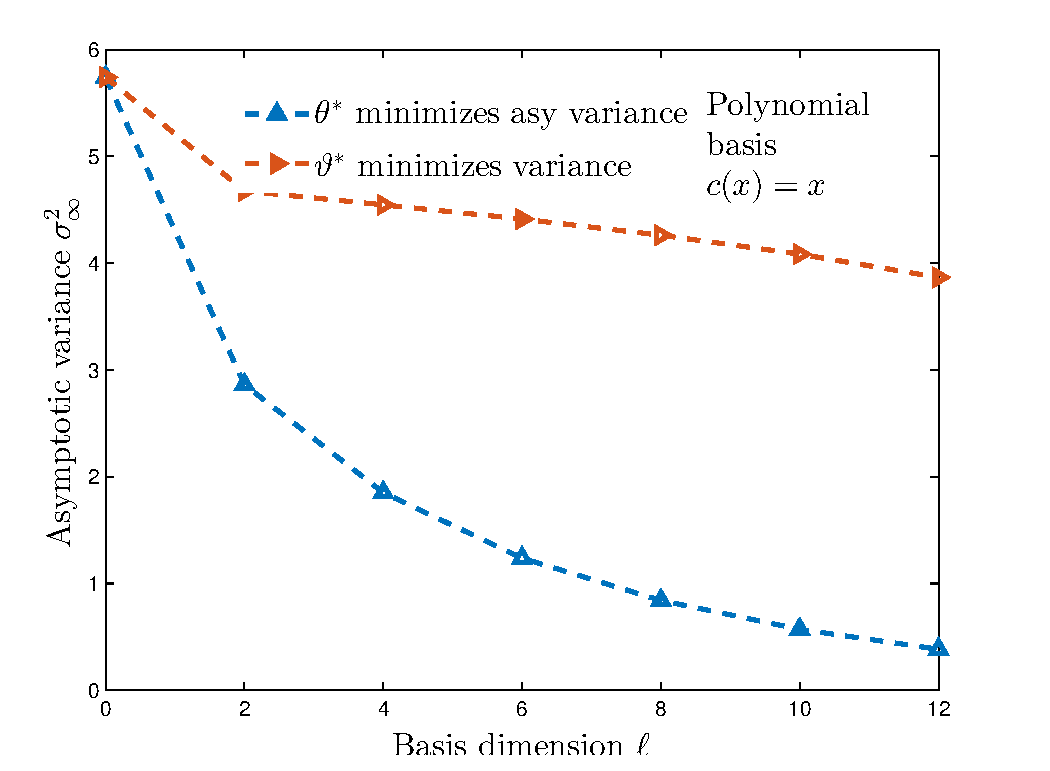
\includegraphics[width=3in]{images/Chap5_x_var_vs_asym_var_poly}} \quad
	\subfigure[]{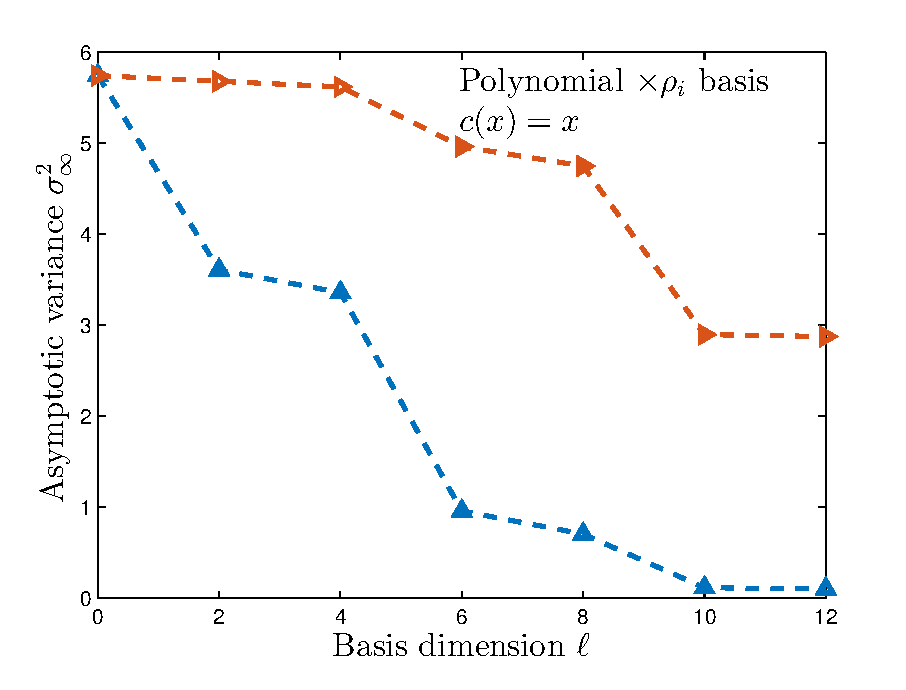
\includegraphics[width=3in]{images/Chap5_x_var_vs_asym_var_wt_poly}}
	% \subfigure[]{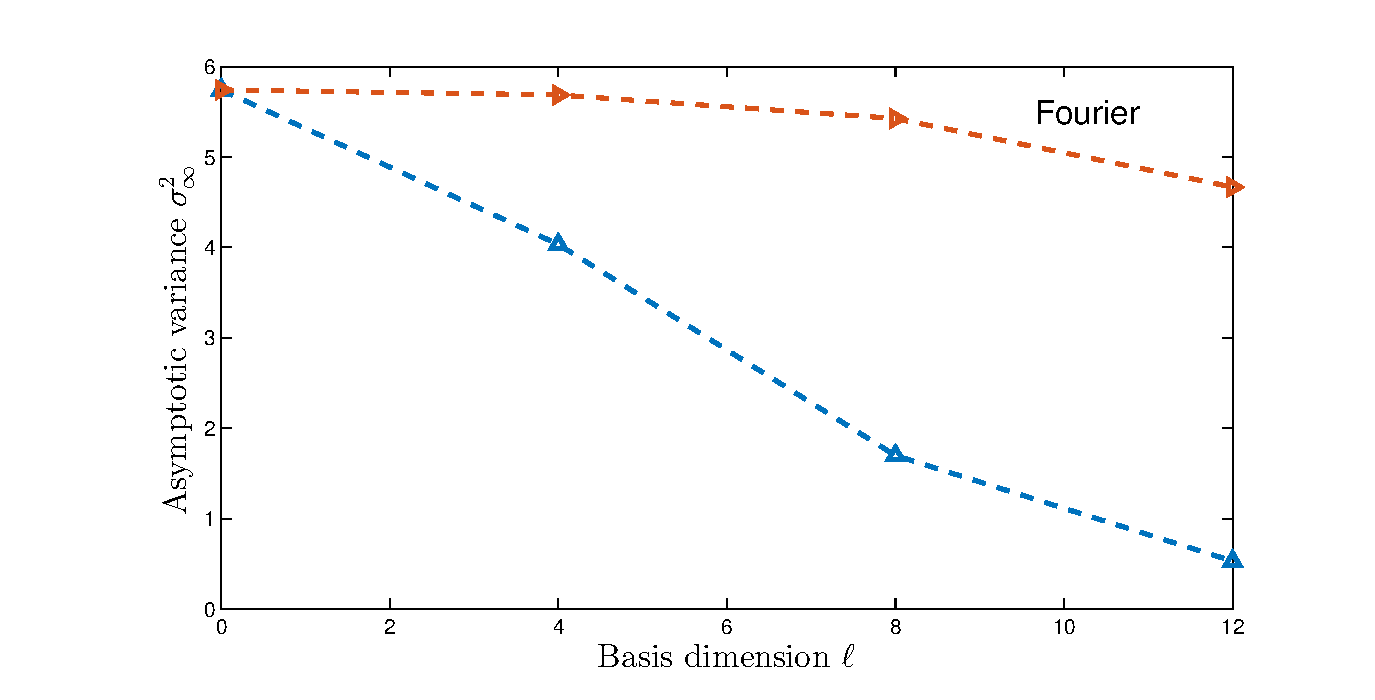
\includegraphics[width=3in]{images/Chap5_x_var_vs_asym_var_fourier}} 
	}

	\mbox{
	\subfigure[]{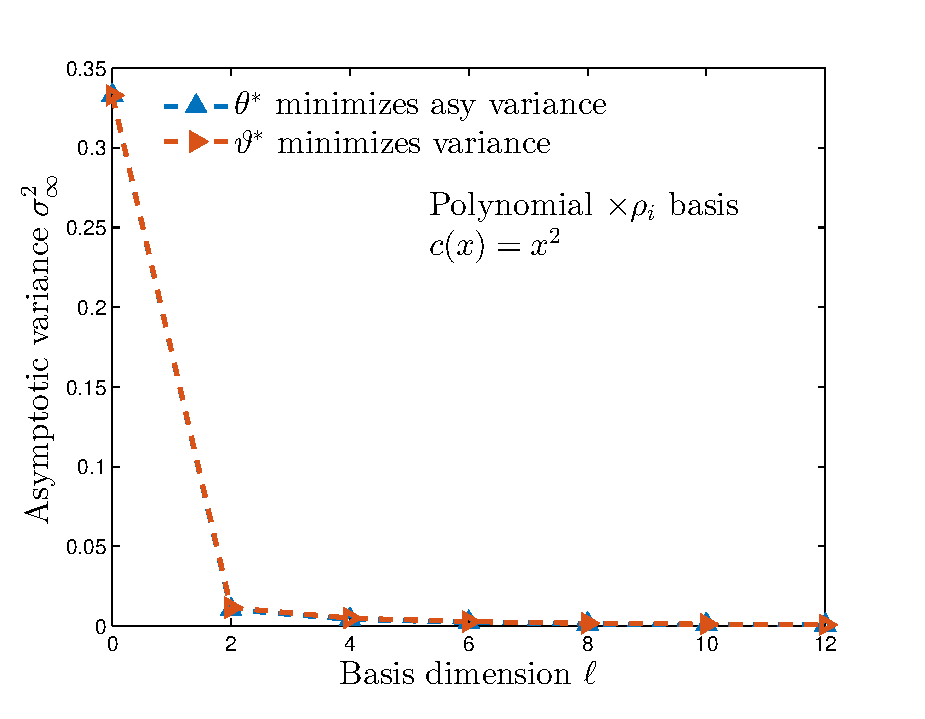
\includegraphics[width=3in]{images/Chap5_x2_var_vs_asym_var_poly}} \quad 
	\subfigure[]{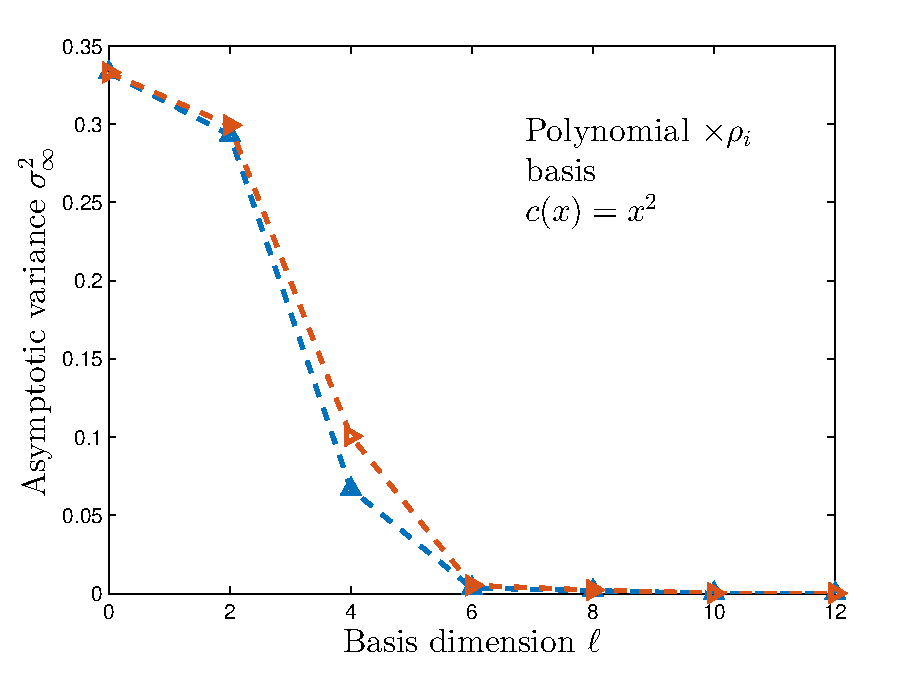
\includegraphics[width=3in]{images/Chap5_x2_var_vs_asym_var_wt_poly}}
	% \subfigure[]{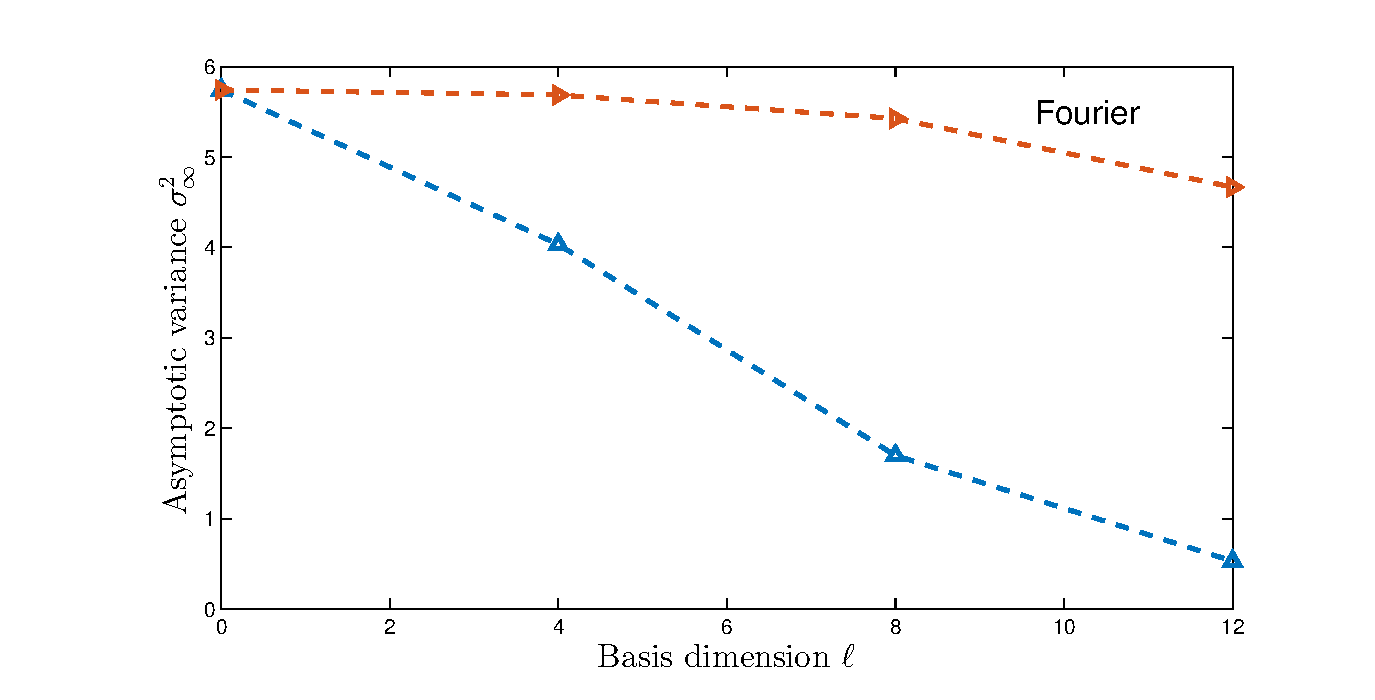
\includegraphics[width=3in]{images/Chap5_x_var_vs_asym_var_fourier}} 
	}
	\caption{Comparison of ${\asymvar}_{,\theta^*}$ and ${\asymvar}_{,\vartheta^*}$ for $\theta^*, \vartheta^* \in \Re^{\ell}$, $0 \leq \ell \leq 12$ and $c(x) = x, x^2$, for i) a polynomial basis (in A and C) and ii) a weighted polynomial basis (in B and D)}
	\label{fig:mcmc_var_vs_asym_var}
\end{figure}

The resulting asymptotic variances for the parameters, $\theta^*$ \eqref{e:mcmc_theta_star} and $\vartheta^*$ \eqref{e:mcmc_var_theta_star} are compared against the basis dimension $\ell$.  The optimality gap for $c(x) = x$, shown in parts A and B of \Fig{fig:mcmc_var_vs_asym_var} is considerable.
The discrepancy is clear from a close look at the two functions $c^{\theta^*}$ and $c^{\vartheta^*}$ that are plotted in \Fig{fig:mcmc_cv_theta_var}. The key difference is that the ``local mean'' of $c^{\theta^*}$ is nearly $\eta$ in each well of the density $\pr$ (shaded region of \Fig{fig:mcmc_cv_theta_var}):
\[
\begin{aligned}
\int_{-\infty}^0 c^{\theta^*}(x) \pr(x)\, dx	
\approx
\int_0^\infty c^{\theta^*}(x) \pr(x) \, dx \approx \eta =0.
\end{aligned}
\]
This helps reduce the asymptotic variance for this slowly mixing diffusion. The function $c^{\vartheta^*}$  does not share this property and produces biased estimates of $\eta$ in each well.
The approximations ${h^{\vartheta^*}}'$ and ${h^{\theta^*}}'$ are plotted along with the exact solution $h'$ obtained analytically in
\Fig{fig:mcmc_cv_theta_var}.  The function ${h^{\vartheta^*}}'$ is a poor approximation to $h'$,  and that results in much higher asymptotic variance. In summary, to minimize the asymptotic variance, it is  important to approximate $h'$ quite well and the $\gradTD$ objective function aims to minimize the approximation error in the mean-square sense. The same experiment was repeated for $c(x) \equiv\sin x$ with similar results. It is conjectured that this phenomenon is more pronounced in multimodal densities. However, for $c(x) = x^2$, both the methods achieve nearly similar reduction in asymptotic variance. 

\begin{figure}[htbp]
	\centering
	\mbox{
		\subfigure []	{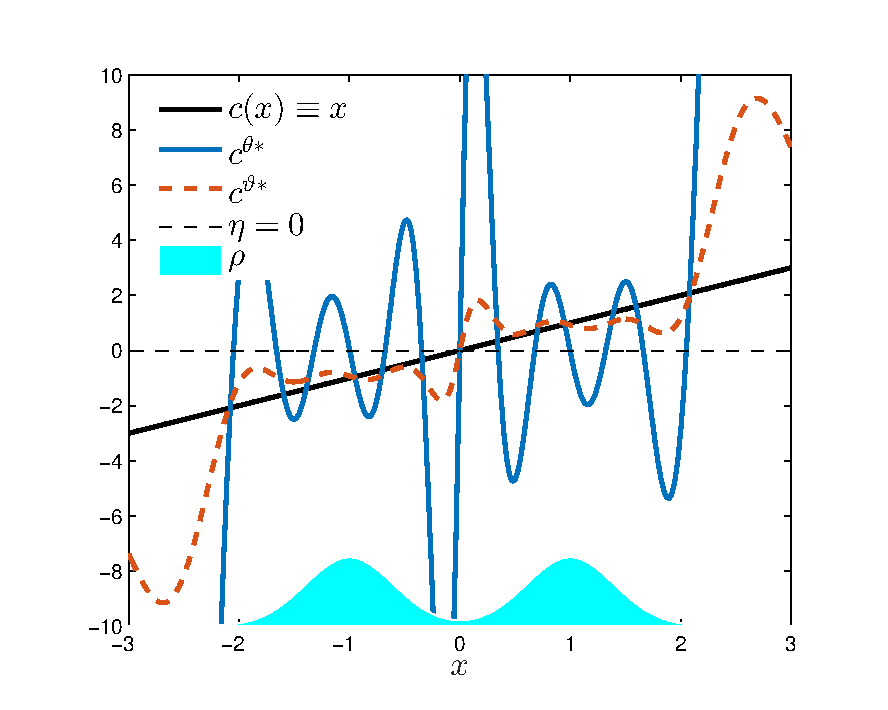
\includegraphics[width=3in]{images/Chap5_x_cvs}} \quad
		\subfigure [] {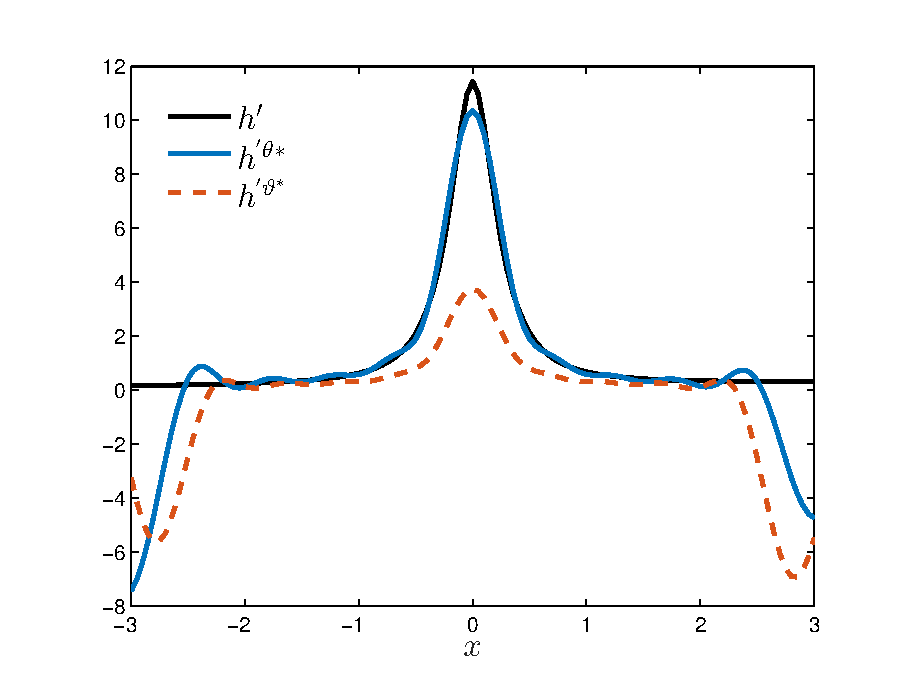
\includegraphics[width=3in]{images/Chap5_x_h_comparison}} 
	}
	\caption{i) Modified estimators using control variates $c^{\theta^*}$ and $c^{\vartheta^*}$, ii) Approximations $h'^{\theta^*}$ and $h'^{\vartheta^*}$ plotted with true gradient $h'$ for $c(x) =x$ with a polynomial $\times \rho_i$ basis.}
	\label{fig:mcmc_cv_theta_var}
\end{figure}


Examining the autocorrelation functions offers another perspective to verify if the two objectives are equivalent. In the discrete time case, the asymptotic variance of the estimates of $\eta$ can be written as the infinite sum of all the autocorrelation functions,
\begin{equation}
\begin{aligned}
\asymvar  & \eqdef \sum_{n=-\infty}^\infty R(n), \qquad R(n) = \Expect [\tilc(\markovstate_0) \tilc(\markovstate_n)] \\
& = 2 \sum_{n=0}^\infty R(n)- R(0).
\end{aligned}
\label{e:mcmc_autocorrelation}
\end{equation}
The expression for $\asymvar$ in \eqref{e:mcmc_avar_reversible} can be derived from this infinite summation form. On inspecting the two objectives, it is easy to see that while $c^{\theta^*}$ tries to minimize $\asymvar$, $c^{\vartheta^*}$ minimizes just the term $R(0)$ in it. This is evident from the the autocorrelation function $R(n)$ in \eqref{e:mcmc_autocorrelation} plotted in \Fig{fig:mcmc_auto_correlation}. Autocorrelation function corresponding to the three different estimators $c,c^{\theta^*}$  and $c^{\vartheta^*}$ for $c(x) = x$, are plotted for $n$ upto $100$. Although, $c^{\vartheta^{*}}$ has the least correlation value at $n=0$ (variance), it shows a slow decay as $n$ increases, $c^{\theta^*}$ shows a much sharper decay in the tails, resulting in a much lower overall asymptotic variance. The plot clearly illustrates that minimizing the variance is not always equivalent to minimizing the asymptotic variance.

\begin{figure}[htbp]
	\centering
	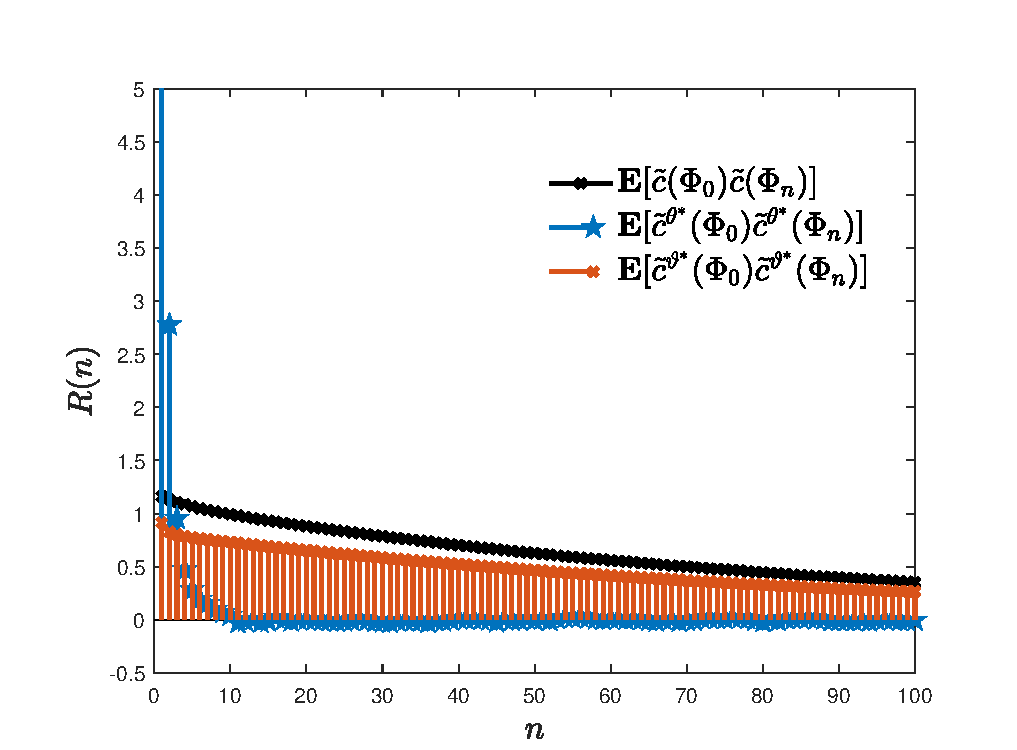
\includegraphics[width=3.5in]{images/Chap5_cov_R_n_gamma_pt05}
	\caption{ Autocorrelation functions $R(n)$ corresponding to the three estimators $c, c^{\theta^*}$ and $c^{\vartheta^*}$  for $n= 0$ to $100$ for ULA with step size $\mcmcstep = 0.05$}
	\label{fig:mcmc_auto_correlation}
\end{figure}

\section{Numerical Examples}
\label{s:mcmc_numerics}
In this section we present a survey of the numerical experiments performed based on the algorithms presented in this paper. We illustrate the remarkable reduction in asymptotic variance that is achieved by the various $\gradTD$ based algorithms, first for estimating the mean of a simple functions $c(x)$ with respect to a univariate Gaussian mixture target density and then in a maximum-likelihood parameter estimation problem using logistic regression.   

\subsection{ULA and RWM for a Univariate Gaussian Mixture Target Density}
\label{s:mcmc_ex_avar}
In this section, we first look at how the control variates are effective in reducing the asymptotic variance for both the ULA and RWM algorithms.  For a simple demonstration of the idea, we consider the same one dimensional bimodal target density defined as mixture of Gaussians \eqref{e:fpf_gaussian_mixture_example}. This gives a symmetric density $\pr$ as shown by the shaded region in \Fig{fig:mcmc_cv_theta_var}. The linear function $c(x) \equiv x$ is used in the simulation experiments; symmetry of $\pr$ and $c$ being an odd function imply $\eta = 0$.

\begin{figure}[htbp]
	\centering
	\mbox{
  	\subfigure[] {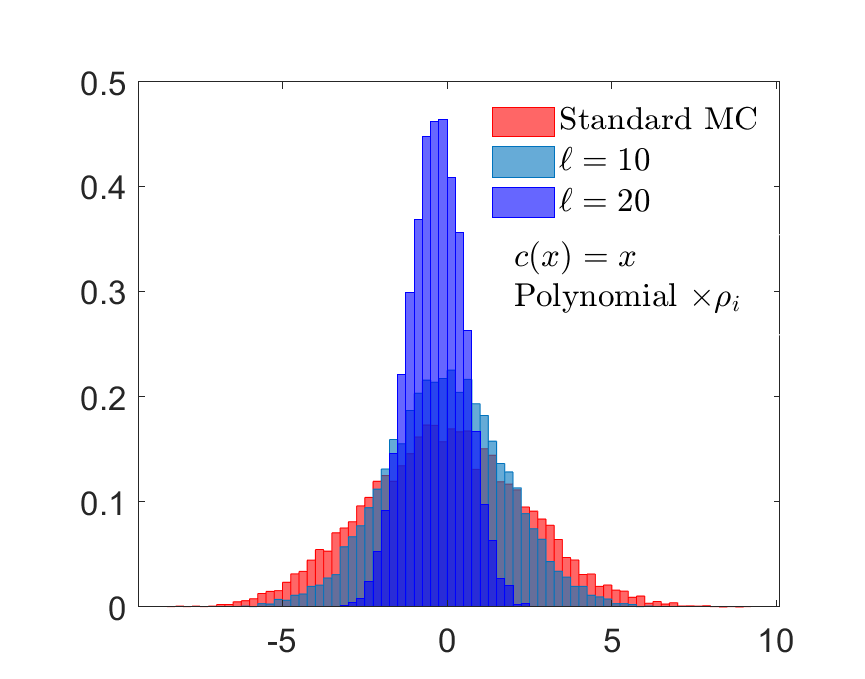
\includegraphics[width=3in]{images/Chap5_hist_all_ds_basis_10000runs_100000samples}}
  	\subfigure[] {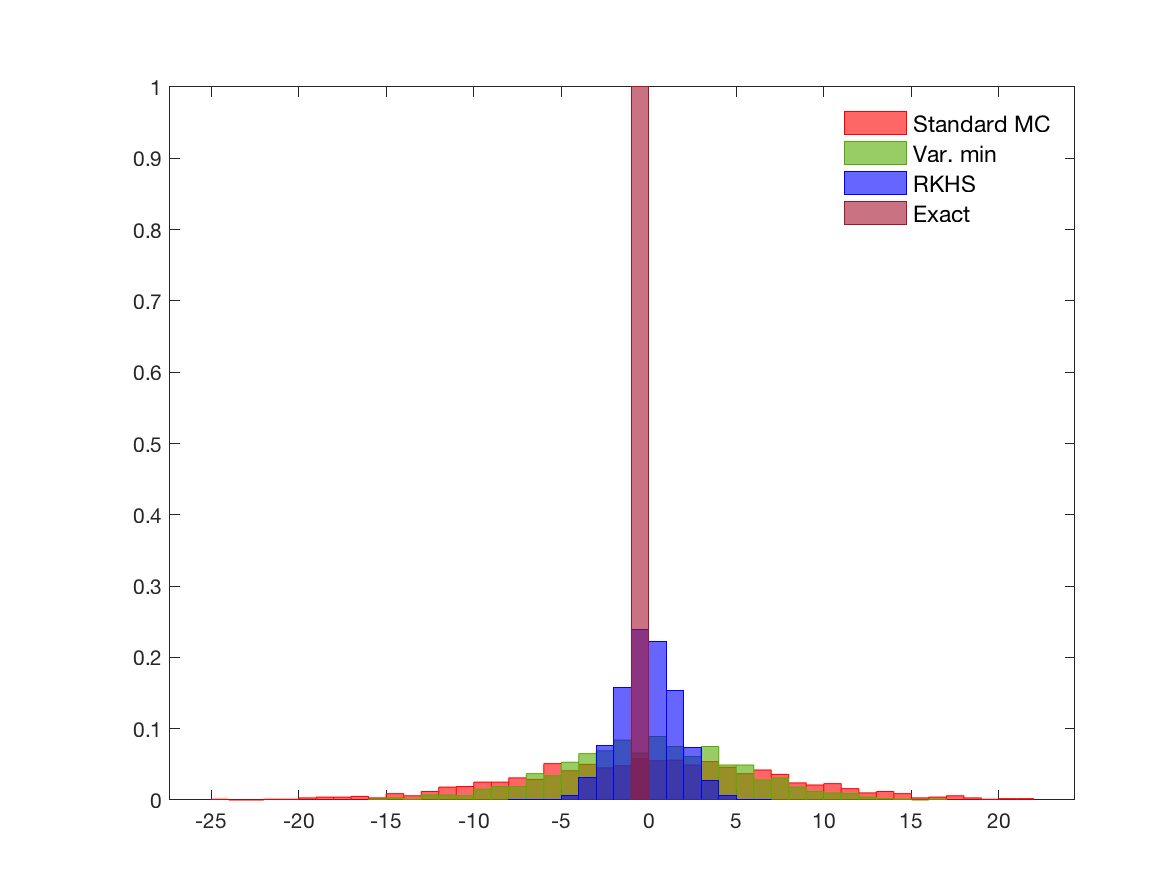
\includegraphics[width=3in]{images/Chap5_hist_asym_var_all_methods}}
  }
 \mbox{
	\subfigure [] {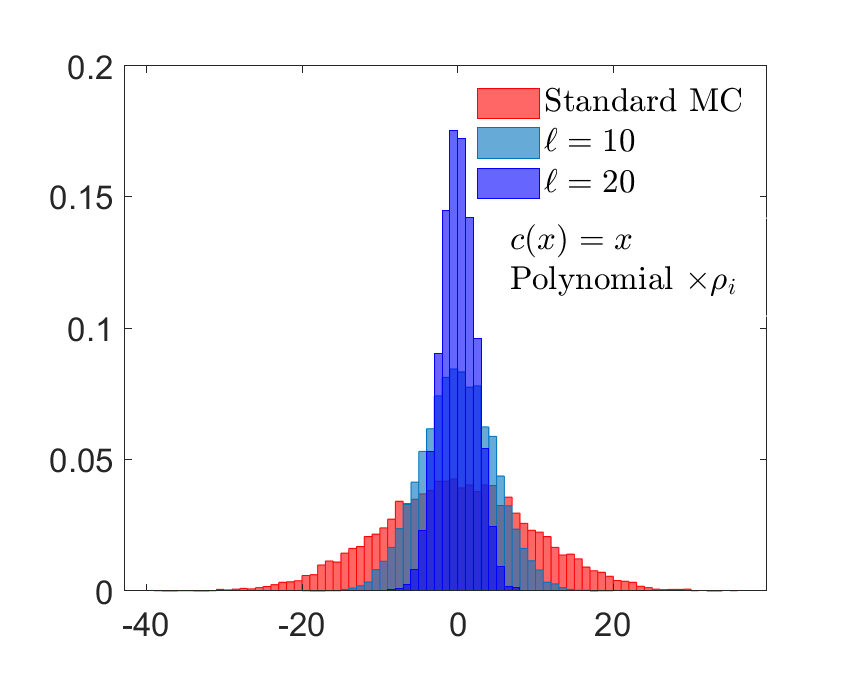
\includegraphics[width = 3in]{images/Chap5_hist_mh_all_ds_basis_10000runs_100000samples}} 
	\subfigure[]	{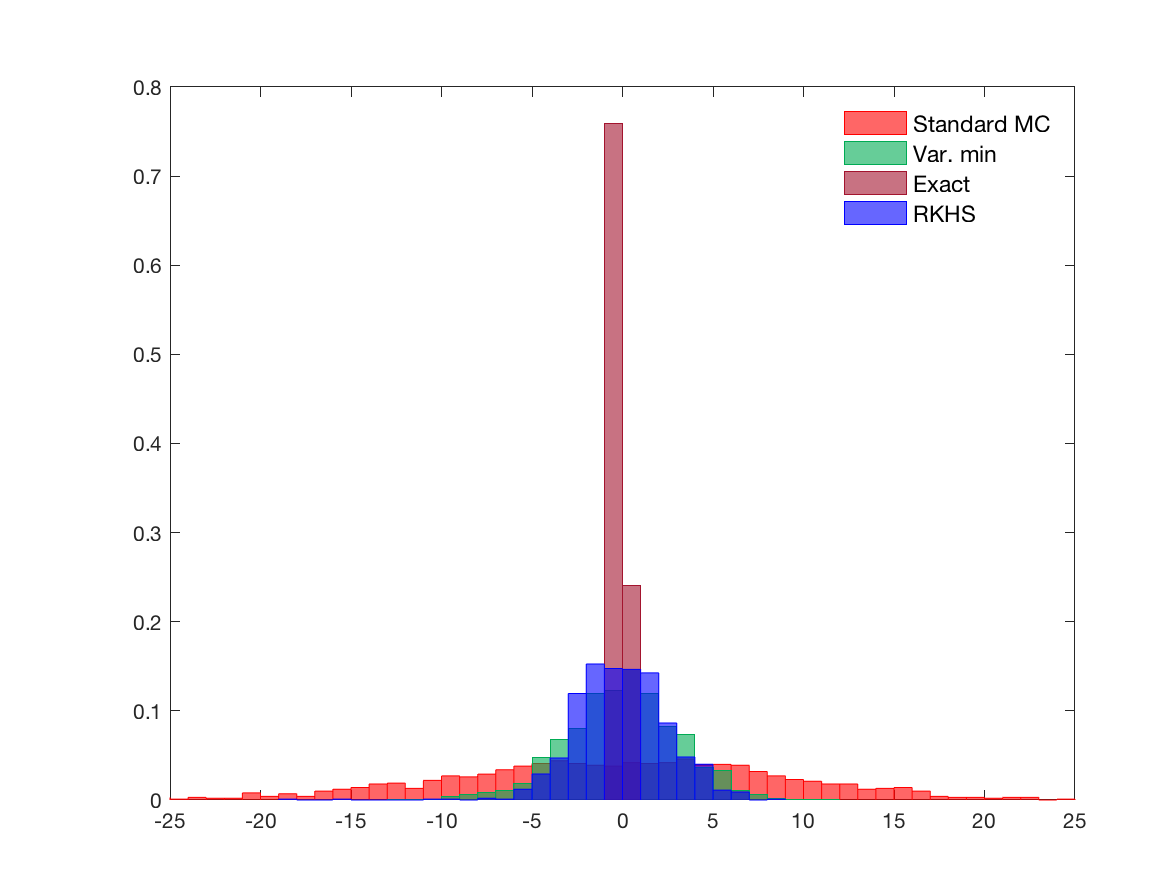
\includegraphics[width=3in]{images/Chap5_hist_mh_asym_var_all_methods}}
 } 
	\caption{Histogram of $\sqrt{N}(\eta_N^{i} - \eta$) for the various control variate schemes -  A) and B) ULA with $\mcmcstep =0.05$ and $c(x) = x$ with finite basis $\ell = 10,20$ in A) and other approximation schemes in B), and C) and D) for RWM with $\mcmcstep = 0.05$ with finite basis $\ell = 10,20$ in C) and other approximation schemes in D).$\ell =0$ corresponds to the standard MCMC estimator.}
	\label{fig:mcmc_ula_rwm_hist}
\end{figure}

Both the ULA and RWM algorithms were simulated using Euler discretization with a step size of $\mcmcstep = 0.05$. Part A in \Fig{fig:mcmc_ula_rwm_hist} shows the histograms of the estimates obtained over $10^4$ independent trials for $\ell= 10,20$ for a weighted polynomial basis, compared to the standard MC estimator. A total number of $10^5$ samples were used in each trial. The empirical variance values observed on the histograms are very close to the analytical variances, although a small bias is seen in the estimate in some cases. This bias may be attributed to the Euler-discretization of the Langevin diffusion which alters the invariant distribution as mentioned in \cite{robtwe96}.  %\Fig{mean_estimate_lang} compares the trajectories of the mean estimate using the standard ULA technique and the improved estimator with the control variates. The improved estimator shows quicker convergence to the actual mean $\eta$ and far fewer fluctuations than the one using the standard technique.

Part B of \Fig{fig:mcmc_ula_rwm_hist} presents a comparison of the performance of the control variates obtained by the other approximation schemes. The histograms were obtained from $1000$ independent trials and the number of samples used in each trial was $N=10^5$. The asymptotic variance obtained by using the exact function $h'$ obtained analytically \eqref{e:fpf_gain_1d} is nearly zero. The $\gradTD$-RKHS algorithm produces the lowest asymptotic variance among approximation methods. Compared to the standard estimator, the variance minimization method (ZV) \cite{papmirgir14} produced nearly the same variance. Markov semigroup approximation method \cite{tagmeh16a} and the constant approximation to $h'$ were also tested, but they produced variances larger than the standard estimator.

The same set of experiments is repeated for the RWM algorithm with the results displayed in parts C and D of \Fig{fig:mcmc_ula_rwm_hist}. Significant reduction in the variance is observed in simulation results. % The intuitive explanation is because of the fact that in the design of $c^\theta$, we try to track $c$ closely using $\generate h^\theta$. Minimizing the error between $h$ and $h^\theta$ tends to minimize the asymptotic variance. In the case of  perfect tracking, $c^\theta$ reduces to the exact mean $\eta$.

\begin{figure}[htbp]
	\centering
		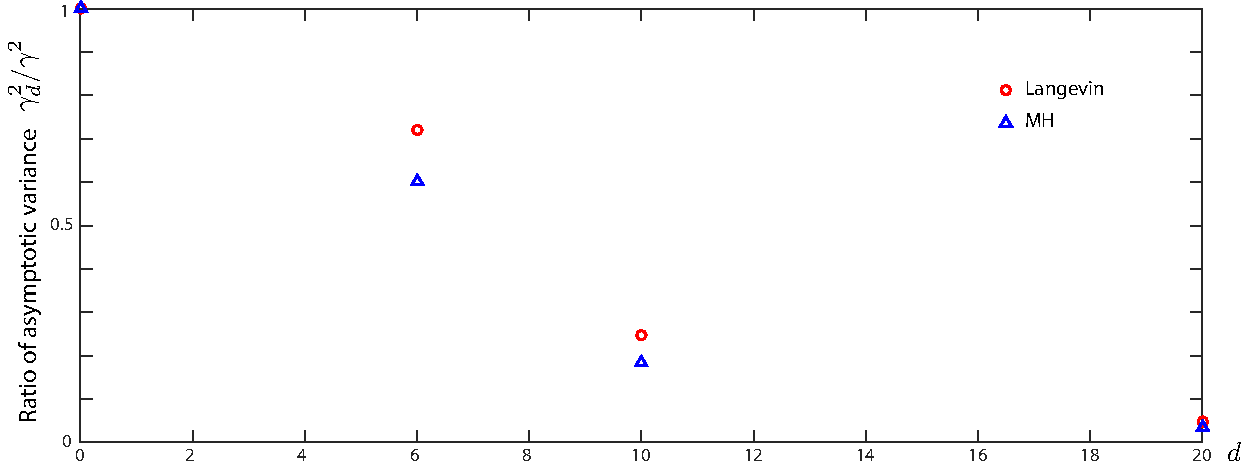
\includegraphics[width=3in]{images/Chap5_rel_red_lang_mh_all}
\caption{Asymptotic variance reduction comparison between ULA and RWM algorithms for $c(x) =x$ and $1\leq \ell \leq 20$}
\label{fig:mcmc_ula_rwm_asy_var}
\end{figure}
\Fig{fig:mcmc_ula_rwm_asy_var} shows the relative reduction in variance for both the ULA and RWM algorithms. The value corresponding to $\ell = 0$ is normalized to $1$ in both the cases. It may be seen that significant variance reduction is achieved for RWM, although at a reduced rate than for ULA. The algorithm can be applied to a wider class of densities with similar results %; we have seen positive results for heavy-tailed densities also. %  Similar trends can also be observed in the Metropolis-Hastings case. \rd{Better results are expected for the Metropolis-Hastings example by applying the algorithm described in \Section{s:cv_reversible_mc}.}

\subsection{Logistic Regression - Swiss Bank Notes Example}
In practice, MCMC algorithms find wide applications in Bayesian inference problems, where we are interested in estimating the mean with respect to a posterior distribution. In this section, we discuss a particular example of Bayesian logistic regression or the logit model. A detailed description of the problem in the context of the Swiss bank notes example is given in \cite{papmirgir14} and a brief summary is provided here.

The goal is to learn the regression coefficients that can be used to classify the Swiss bank notes dataset into genuine and counterfeit. Given in the dataset are the measurements for four covariates - the length of the bill, the width of the left and the right edges and the bottom margin width for 200 bank notes of which 100 each are counterfeit and genuine. This is essentially a binary classification problem in a supervised learning setting. 

Let $X \in \Re^{N_n \times N_d}$ correspond to the covariate measurements of $N_n$ bank notes, with $N_d$ denoting the number of covariates with $N_n = 200$ and $N_d = 4$. Let $\{Y_i  \in \{0,1\}, 1 \leq i \leq N_n \}$ correspond to the labels for each note being genuine or counterfeit respectively. Let $\boldsymbol{\Theta} \in \Re^{N_d}$ be the regression coefficients that are learned from the given data. We are interested in finding the best estimates for the regression coefficients, i.e. the coefficients that maximize the posterior probability $\pr$ defined as,
\begin{equation}
\begin{aligned}
\boldsymbol{\Theta}^* &\eqdef  \argmax_{\Theta \in \Re^{N_d}} \pr(\boldsymbol{\Theta}| \{X_i,Y_i\}_{i=1}^{N_n}) \\
&= \argmax_{\Theta \in \Re^{N_d} }\exp\left( \underbrace{\sum_{i=1}^{N_n} \{Y_i \boldsymbol{\Theta}^\transpose X_i - \log(1+e^{\boldsymbol{\Theta}^\transpose X_i} ) \}}_{\text{Likelihood}} - \underbrace{2^{-1} \boldsymbol{\Theta}^\transpose \Sigma^{-1} \boldsymbol{\Theta}}_{\text{prior}} \right),
\end{aligned}
\label{e:mcmc_log_reg}
\end{equation}
where the parameter vector $\boldsymbol{\Theta} = [ \Theta_1, \dots ,\Theta_{N_d}]$ has a zero-mean Gaussian prior with a covariance matrix $\Sigma$.

In problems such as this, the maximum a posteriori (MAP) estimate is rarely available in closed-form and is hard to compute. Instead, we try to compute the Bayesian estimate: 
\begin{equation}
\boldsymbol{\Theta}_{{bayes}} \eqdef \int_{\Theta \in \Re^{N_d}} \boldsymbol{\Theta} \, \pr(\boldsymbol{\Theta}| \{X_i,Y_i\}_{i=1}^{N_n}) \ud \Theta.
\label{e:mcmc_log_reg_bayes}
\end{equation}
Obtaining the Bayesian estimator \eqref{e:mcmc_log_reg_bayes} requires sampling $\boldsymbol{\Theta}$ values from the posterior distribution and then computing the empirical mean $\hat{\boldsymbol{\Theta}}$. Samples from this posterior density may be obtained using any reversible MCMC technique, in particular we focus on the RWM algorithm. In the following, it is assumed that $N$ samples generated by the RWM algorithm are available.

The goal as before is to compute the optimal control variates that minimize the asymptotic variance of each of the estimates $\hat{\boldsymbol{\Theta}}$.
Optimal control variates can be obtained from approximate solutions to the following Poisson's equations corresponding to each of the four regression coefficients:
\begin{equation}
\generate h_k = -\tilde{\Theta}_k = - (\Theta_k - \hat{\Theta}_k), \qquad   1 \leq k \leq N_d.
\label{e:poisson_logit}
\end{equation}
The approximation $h^\theta_k$ is chosen to belong to a family of linearly parameterized functions as before,
\[
h^\theta_k \eqdef \theta_k^\transpose \psi =  \sum_{j=1}^\ell \theta_{kj} \psi_j,
\]
where $\psi_j : \Re^{N_d} \to \Re$ is the chosen set of basis functions and $\theta_{kj} \in \Re$ are the parameter values.  The optimal parameter values are obtained by minimizing $ \| \nabla h_k - \nabla h^\theta_k \|^2_{L^2}$. For a general basis, the optimal parameter $\theta_k^*$  can be derived along the same lines as before,
\begin{equation}
\begin{aligned}
\theta_k^*  &= M^{-1} b_k, \qquad \text{where,}\\
M & \eqdef \langle \nabla \psi, \nabla \psi \rangle_{L^2} \approx \frac{1}{N} \sum_{i = 0}^{N-1}\nabla \psi(\boldsymbol{\Theta}^i) \nabla \psi^\transpose(\boldsymbol{\Theta}^i)\\
b_k & \eqdef \langle \tilde{\Theta}_k, \psi \rangle_{L^2} \approx \frac{1}{N} \sum_{i=0}^{N-1}\tilde{\Theta}_k^i \psi(\boldsymbol{\Theta}^i), \\
\label{e:theta_k}
\end{aligned}
\end{equation}
where each $\boldsymbol{\Theta^i}$ corresponds to the $i^{\text{th}}$ sample of the MCMC algorithm

Polynomials of degree $1$ and $2$ are chosen as the basis functions in \cite{papmirgir14} and we use the same basis for comparing the algorithm performances. Additionally, we also compare the results against the $\gradTD$-RKHS algorithm with Gaussian kernels. 

\noindent \subsubsection*{Linear polynomial basis}
First we choose $\ell=4$ and $\psi_j$ to be polynomial of degree $1$, i.e.
\begin{equation}
\psi^\transpose \eqdef [ \Theta_1 \quad \Theta_2 \quad \Theta_3 \quad \Theta_4] := \boldsymbol{\Theta}^\transpose
\label{e:mcmc_log_reg_linear}
\end{equation}
For this choice of $\psi$,  $\nabla \psi = I$ and $ \Delta \psi = 0$. Hence, $\theta^*_k$ has the simple expression,
\begin{equation}
\theta^*_k = \frac{1}{N} \sum_{i=0}^{N-1} \tilde{\Theta}_k^i \boldsymbol{\Theta}^i
\label{e:mcmc_log_reg_theta_lin_poly}
\end{equation}
The control variate $\generate h^\theta_k$ is explicitly computable and is given by,
\[
\generate h^\theta_k(\boldsymbol{\Theta}^i) = -\nabla \log(\pr(\boldsymbol{\Theta}^i|\{X_j,Y_j\}_{j=1}^N)) \cdot \theta^*_k \qquad \forall k, i
\]
and the new estimator of the regression coefficients will be,
\[
\bar{\Theta}^i_k \eqdef \Theta^i_k + \generate h^\theta_k(\boldsymbol{\Theta}^i).
\]
The ZV-MCMC algorithm, proposed in \cite{papmirgir14} minimizes the ordinary variance instead of the asymptotic variance. In general, it is an easier optimization problem to solve, but in this specific example, it is interesting to note that $\theta_k^*$  using \eqref{e:mcmc_log_reg_theta_lin_poly} is simpler to compute and the solution is numerically more stable (as inverting an ill-conditioned matrix is not required) than the ZV method. This is denoted as $\gradTD$-L in the plots in \Fig{fig:mcmc_box_plots_Theta}. 

\noindent \subsubsection*{Quadratic basis}
A quadratic polynomial basis of the form,
\begin{equation}
\psi^\transpose \eqdef [\Theta_1, \, \Theta_2, \, \Theta_3, \, \Theta_4, \, \Theta_1^2, \, \Theta_1 \Theta_2, \, \Theta_1\Theta_3, \, \Theta_1 \Theta_4, \, \Theta_2^2, \, \Theta_2\Theta_3, \, \Theta_2\Theta_4, \, \Theta_3^2, \, \Theta_3 \Theta_4, \, \Theta_4^2] 
\label{e:mcmc_log_reg_quadratic}
\end{equation}
is also considered similar to \cite{papmirgir14}.  In this case, $\nabla \psi \in \Re^{14 \times 4}$ and $\theta_k \in \Re^{14}$. The optimal parameter values are given by \eqref{e:theta_k}. This is denoted as $\gradTD$-Q in the plots in \Fig{fig:mcmc_box_plots_Theta}.

\noindent \subsubsection*{$\gradTD$-RKHS algorithm}
We also investigate the performance of the RKHS based $\gradTD$ learning algorithm for this example.  The parameter values of $\lambda = 10^{-7}$ and $\epsy = 2$ were found to produce the best results.  As it becomes prohibitively expensive to place a Gaussian kernel at each of the RWM samples, they were placed at $200$ randomly chosen samples.
\noindent \subsection*{Results}
Simulations were performed using the Swiss bank note dataset provided in \cite{papmirgir14}. We performed $1000$ independent trials each with  $10^5$ samples and $10^4$ samples used for burn-in. The box plots of the estimates of the four regression coefficients $\boldsymbol{\Theta}$ shown in \Fig{fig:mcmc_box_plots_Theta} indicate that significant variance reduction is  achieved using all the control variate methods. It may be observed that for a linear basis, both the ZV-L and $\gradTD$-L learning produce nearly the same asymptotic variance. The $\gradTD$ method is able to produce estimates for the four regression coefficients, whose variance values are $10-65$ times smaller than the standard RWM sampler. Using the quadratic polynomial basis, ZV-Q method outperforms the $\gradTD$-Q method slightly, a variance reduction factor of $100-200$ over the standard estimator is still obtained. The $\gradTD$-RKHS method produces the best results with variances that are lower by a factor $20-50$ over the ZV-Q method. The $\gradTD$-RKHS method however produced a much larger number of outliers. By a more careful choice of the values for $\lambda,\epsy$ and by placing the kernel functions at more well-chosen samples, better results may be obtained.

\begin{figure}[htbp]
	\centering
	\mbox{
		\subfigure [] {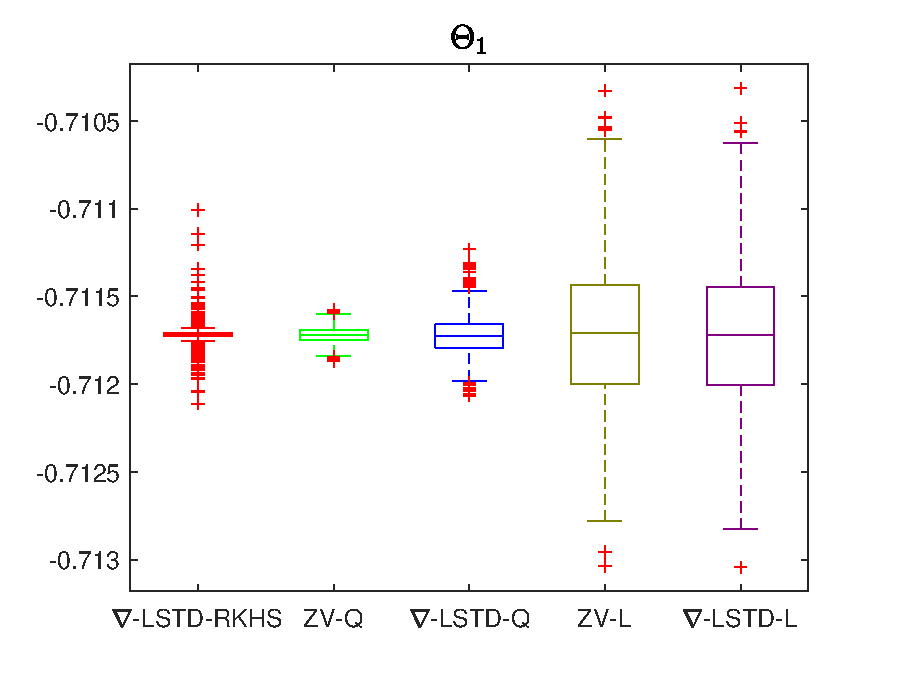
\includegraphics[width=3.25in]{images/Chap5_hist_Theta1_no_std}}
		\subfigure [] {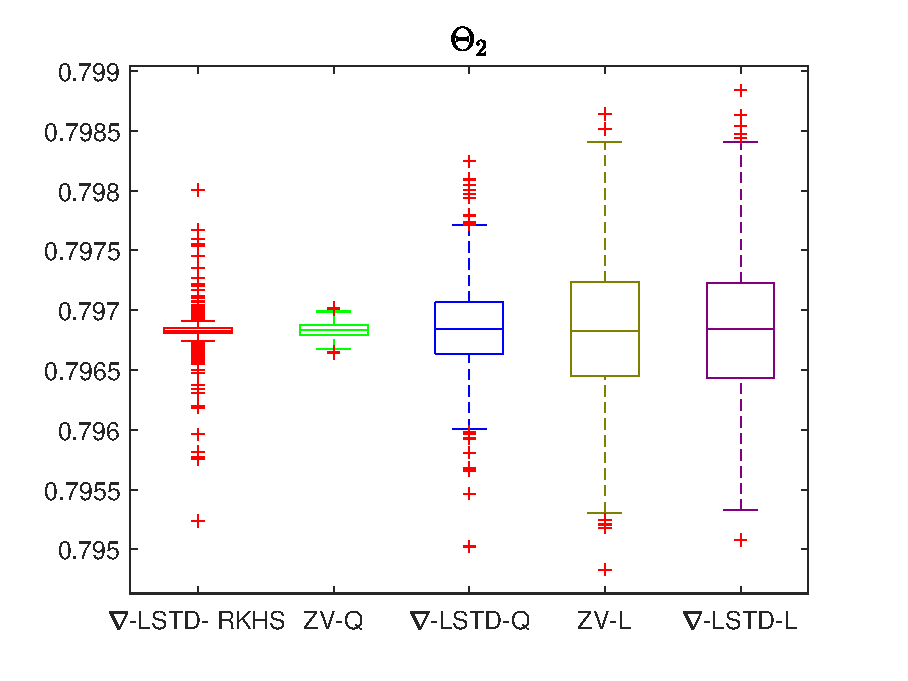
\includegraphics[width=3.25in]{images/Chap5_hist_Theta2_no_std}} 
	}
	\mbox{
		\subfigure [] {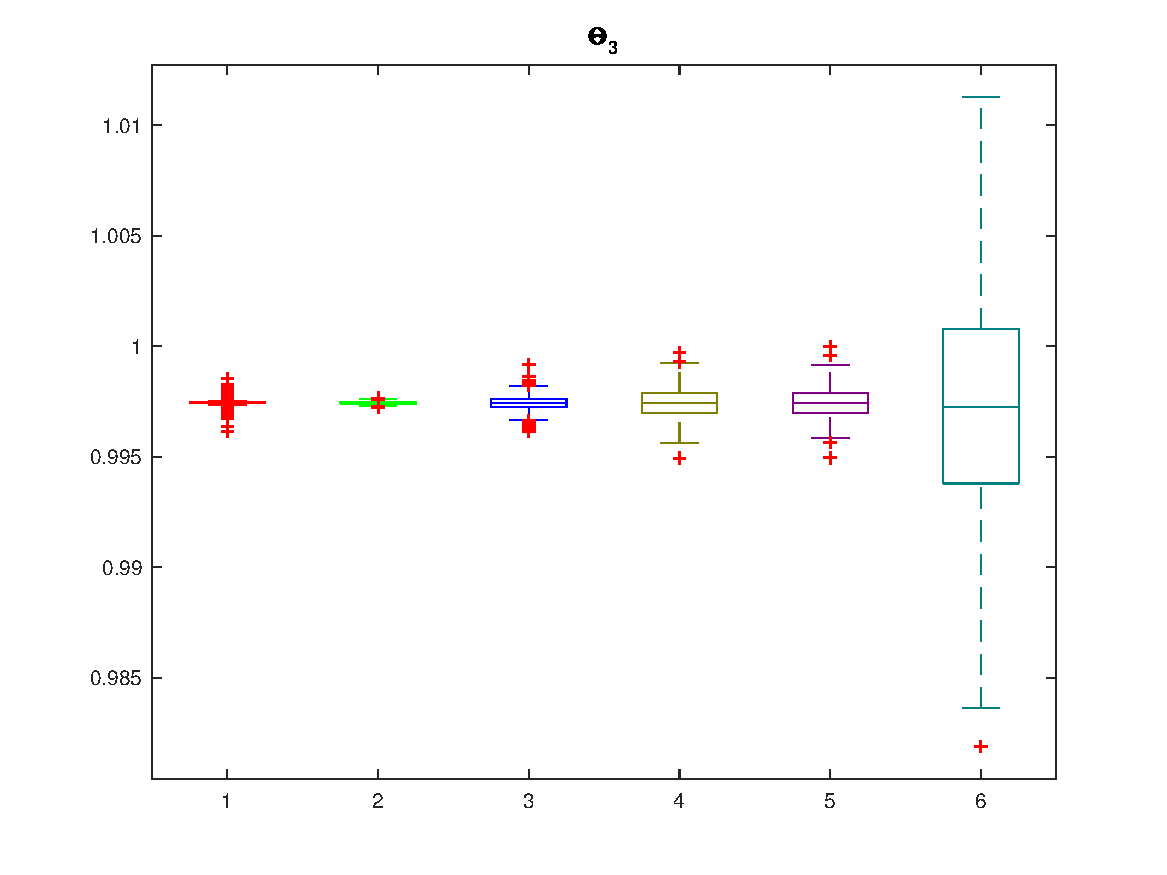
\includegraphics[width = 3.25in]{images/Chap5_hist_Theta3_no_std}} 
		\subfigure [] {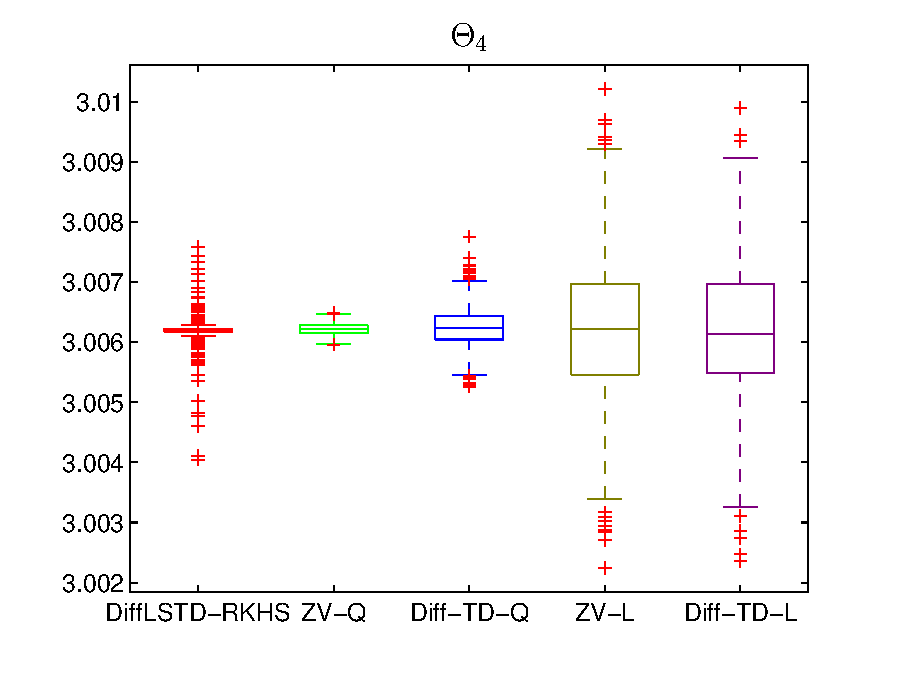
\includegraphics[width = 3.25in]{images/Chap5_hist_Theta4_no_std}} 
	} 
	\caption{Boxplots of estimates of $\boldsymbol{\Theta}$ obtained over 1000 trials using linear and quadratic polynomial basis using the ZV-MCMC and $\gradTD$ and the $\gradTD$-RKHS algorithms).}
  \label{fig:mcmc_box_plots_Theta}
\end{figure}

One might also be interested in the ordinary variance of the samples within a single run. The box plots in \Fig{fig:mcmc_box_var_Theta} compare the variance values of the samples obtained within a run using the ZV-Q method and the $\gradTD$-RKHS learning method. It may be observed that in spite of having outliers, the mean variance using the RKHS method is about one order of magnitude lower than the ZV-Q method.

The same set of experiments were tried out with similar results for the logistic regression example using MALA and ULA sampling. Similar results were also obtained for the probit model Vaso constriction example discussed in \cite{papmirgir14}. The plots for these simulations are provided in the appendix. %\anand{Should I include those plots?}

\begin{figure}[htbp]
	\centering
	\mbox{
		\subfigure [] {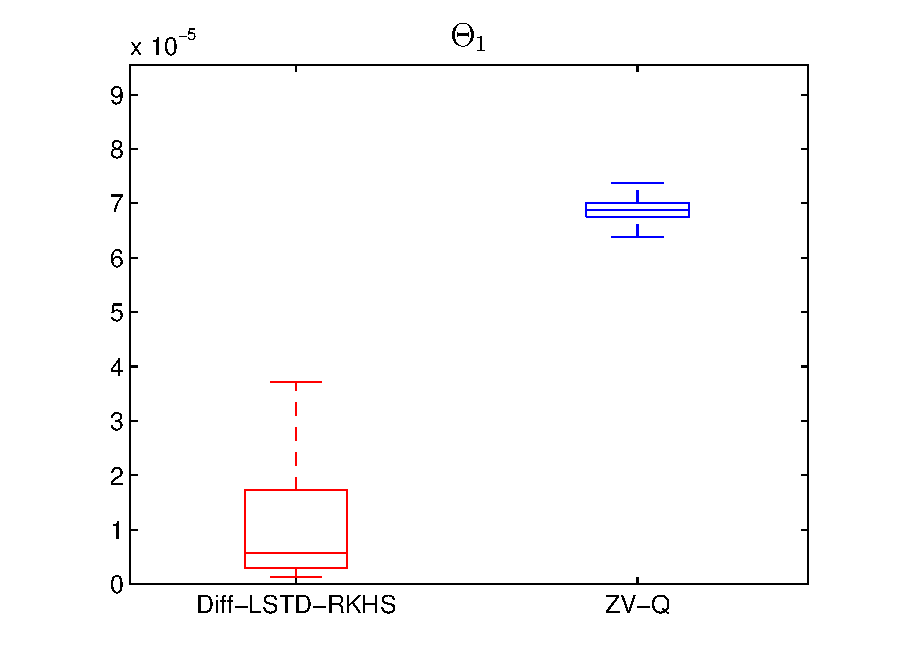
\includegraphics[width=3.25in]{images/Chap5_box_var_Theta1}}
		\subfigure [] {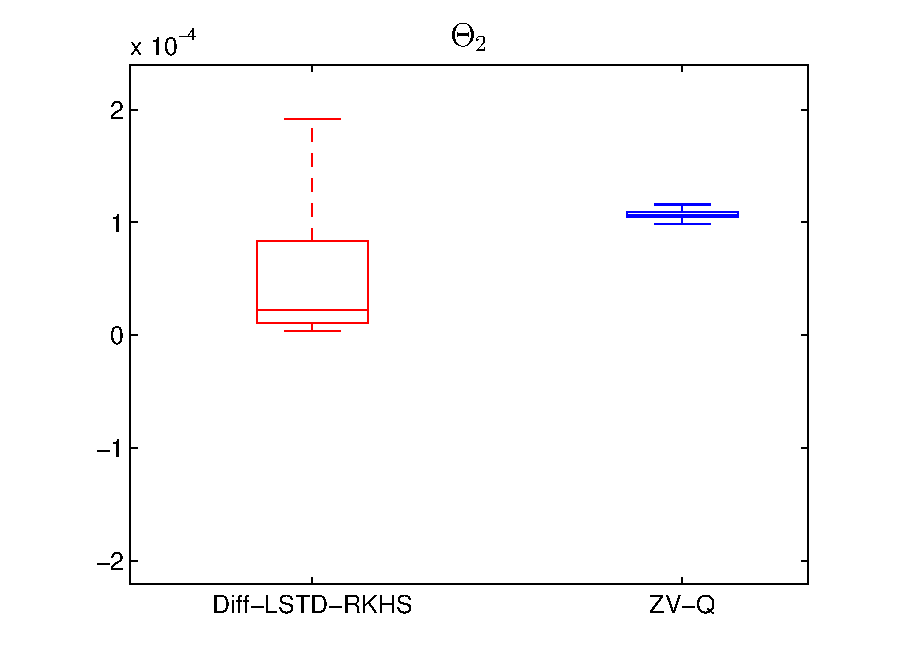
\includegraphics[width=3.25in]{images/Chap5_box_var_Theta2}} 
	}
	\mbox{
		\subfigure [] {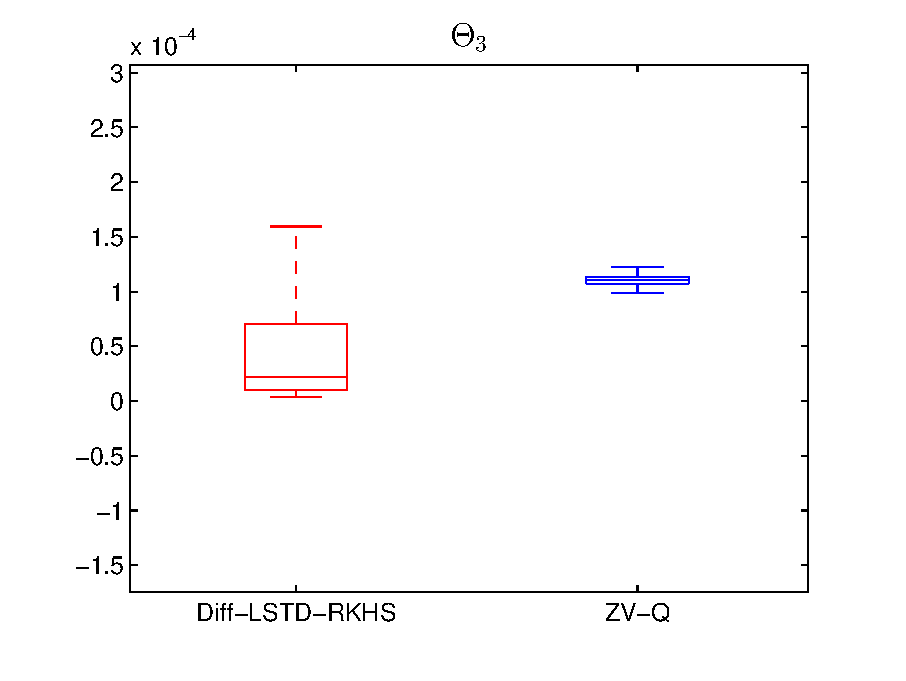
\includegraphics[width = 3.25in]{images/Chap5_box_var_Theta3}} 
		\subfigure [] {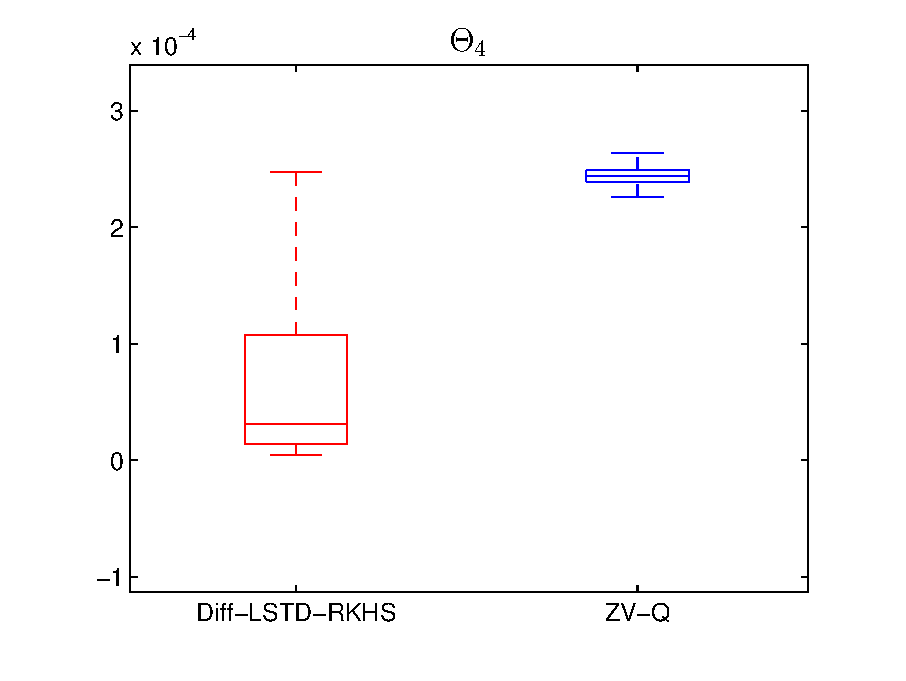
\includegraphics[width = 3.25in]{images/Chap5_box_var_Theta4}} 
	} 
\caption{Boxplots of the in-trial variances of estimates of $\boldsymbol{\Theta}$ obtained over 1000 trials using the $\gradTD$-RKHS and ZV-Q with quadratic polynomials}
\label{fig:mcmc_box_var_Theta}
\end{figure}

\section{Conclusions}
In this chapter, we provided a brief discussion on MCMC algorithms, particularly the ULA, which has an associated continuous time Langevin diffusion process. MCMC algorithms have been widely used in Bayesian inference, as a means of approximating expectations using numerical integration. Asymptotic variance was defined as a measure of convergence of these algorithms. We illustrated using an example that the simpler task of minimizing the variance is not always equivalent to minimizing the asymptotic variance, in fact in certain examples minimizing one quantity produces undesirable results on the other. For the Langevin based algorithms, using \Prop{prop:lang_generator_grad}, we are able to express the asymptotic variance minimization problem in a form that fits into the $\gradTD$ learning objective function. This immediately opens up the application of the various versions of $\gradTD$ learning algorithms discussed in the previous chapters to be applied to this problem. The effectiveness of these techniques is however not limited to ULA, they are also seen to produce significant variance reduction in MALA and RWM algorithms. Through recent research, we have sought theoretical justification for the positive numerical results.  

%\chapter{Conclusions and Future Work}
\label{ch:conclusions}
The objectives of the doctoral research surveyed in this dissertation may have been overly broad,  but to a large extent the goals have been met. The development of $\gradTD$ learning based algorithms was mainly motivated by its application to FPF. Prior to this dissertation, the FPF gain estimation was an open problem. Only constant gain and Galerkin approximations were used in practice. We developed a new class of differential TD learning algorithms, whose applications are not restricted to FPF gain approximation. The discrete-time and finite state space analog of the generic $\gradTD$ algorithm presented here has been applied to optimal control problems like speed scaling in microprocessors \cite{ctcn,devmey16a}. However, the original algorithm was inefficient both statistically and computationally. Statistically, it suffered from high variance issues, and computationally, an additional layer of complexity was introduced which required simulation of the Langevin SDE. This algorithm was also not friendly for online filtering problems as it requires simulating the SDE upto one million samples per filtering time step. \Prop{prop:lang_generator_grad} provided an important breakthrough and helped us develop a $\gradTD$-L version for the Langevin diffusion in Chapter 2. This algorithm yields a more computationally efficient method by reducing particle sizes to $N=500$ or $1000$ from $10^6$. The need to obtain a smooth approximation for the empirical posterior is also avoided. Thus, it is more ``plug and play'' in nature, when applied to a filtering problem.  

However, one major difficulty that remained unsolved is the extension to problems with higher dimensional state spaces. An appropriate choice of a parameterized family of functions is difficult without any insight about the structure of the solution. Basis-independent versions of $\gradTD$ learning algorithms were developed in an RKHS setting. Using a recent extension of the classical representer theorem that includes gradient terms in the loss function, we obtained the best approximations from within an infinite dimensional Hilbert space. The $\gradTD$-RKHS learning algorithms allow easy extensions to higher dimensions. Performance comparison of all these different methods was done in the context of gain function approximation and filtering examples. 

It was also observed that the same algorithms could be applied to minimize the asymptotic variance of MCMC algorithms. For the Langevin diffusion, the asymptotic variance minimization takes an objective function that exactly matches the framework of $\gradTD$ learning. Through recent research, we provide theoretical justification to apply the control variates methods to non-Langevin based algorithms like RWM as well. 

In spite of this, there remains several open research problems, in establishing relevant theory, developing more efficient algorithms, as well as in finding practical applications: 
\begin{romannum}
\item Investigate why the reduced complexity solution is as good as the optimal?\footnote{committee member Prof. J. Princip\'{e} conjectures that a proof of approximately optimality may not be a significant technical challenge}
\item Error analysis in machine learning, and in particular in the context of kernel methods, is an active research topic \cite{boueli02}. We think this would lead to valuable insights on choices of hyper parameters $\reg$ and $\epsy$.
\item A more thorough comparison of the various gain approximation algorithms is also needed.
\end{romannum}

In terms of algorithm development, we should aim for:
\begin{romannum}
\item Developing a $\gradTD$-RKHS algorithm with a differential regularizer. Currently, this is limited by the scope of representer theorem. 
\item Developing an algorithm based on semiparametric representer theorem, that allows the use of additional parameterized functions into the approximating class.
\end{romannum}
In terms of practical applications of the work, we need to investigate:
\begin{romannum}
\item  Real time filtering problems - Potential application to battery SOC estimation is being explored currently. 
\item Applications of FPF to control in the context of partially observed Markov decsion processes.
\end{romannum}

  %These chapters are not included in the template
%\include{tex/chapter7}

%-----------------------------------------------------------------------%

% Use the appropriate file depending upon the number of appendices you have


% % The Editorial Office Requirements for the Table of Contents cause a significant problem
%in Latex if there is only one Appendix. The Appendix is no longer labeled "A" in the TOC
%but has the word "APPENDIX" placed in front of the title of the Appendix. This can be done
%without issue IF nothing needs to be numbered by LaTeX in the Appendix. Unfortunately, most of the time
%something needs to be numbered in that single Appendix. For this reason we have included the IFTHENELSE switch
%found in this document and at the beginning of AppendixA. We assume that if you have any appendices, that you have more than one. However, you DO only have one appendix DO NOT USE THIS FILE!!!!!!!!!!!!!!!!!!!!!!!
%
% OneSingleAppendix.tex has all the settings needed to adjust for a single appendix
% you will have a major problem with your TOC if you use this file with a single appendix!!!!!

%
% Comment (or delete) all of the \input{AppendixB} commands except those you are using.
%Then open the AppendixA.tex file and continue there.

%you can add/substract individual appendices through by using the /include{appendix'X'}
% and creating/deleting the appropriate files
\appendix %
%\clearpage%

\addtocontents{toc}{\protect\addvspace{10pt}\noindent{APPENDIX} \protect\hfill\par}{}


% % % % % % % If you have a single appendix, you should be using appendix1.tex
% % % % % % % NOT this file

\chapter{Orthonormal Basis Functions and Mercer's Theorem}
\label{a:mercers_theorem}

Given an RKHS $\clH$, it is useful to understand the set of functions that belong to the Hilbert space. This can be studied using Mercer's theorem \cite{merrus09}. Mercer's theorem forms the connection between the theory of reproducing kernels and integral operators. 
Consider the integral operator (Hilbert-Schmidt operator) $L_K:L^2_\measure(x) \to L^2_\measure(x)$ defined by,
\begin{equation}
(L_K f)(x) = \int_\state \Kern(x,t) f(t) d\measure(t)
\end{equation}
where $\measure$ is a finite Borel measure and $\state$ is a compact set.
The linear map $L_K^{1/2}$, which denotes the square root of $L_K$ is a Hilbert isomorphism between $L^2_{\measure}(\state)$ and $\clH$ as illustrated in \Fig{fig:rkhs_isomorphism}. 

\begin{figure}[htbp]
	\centering
	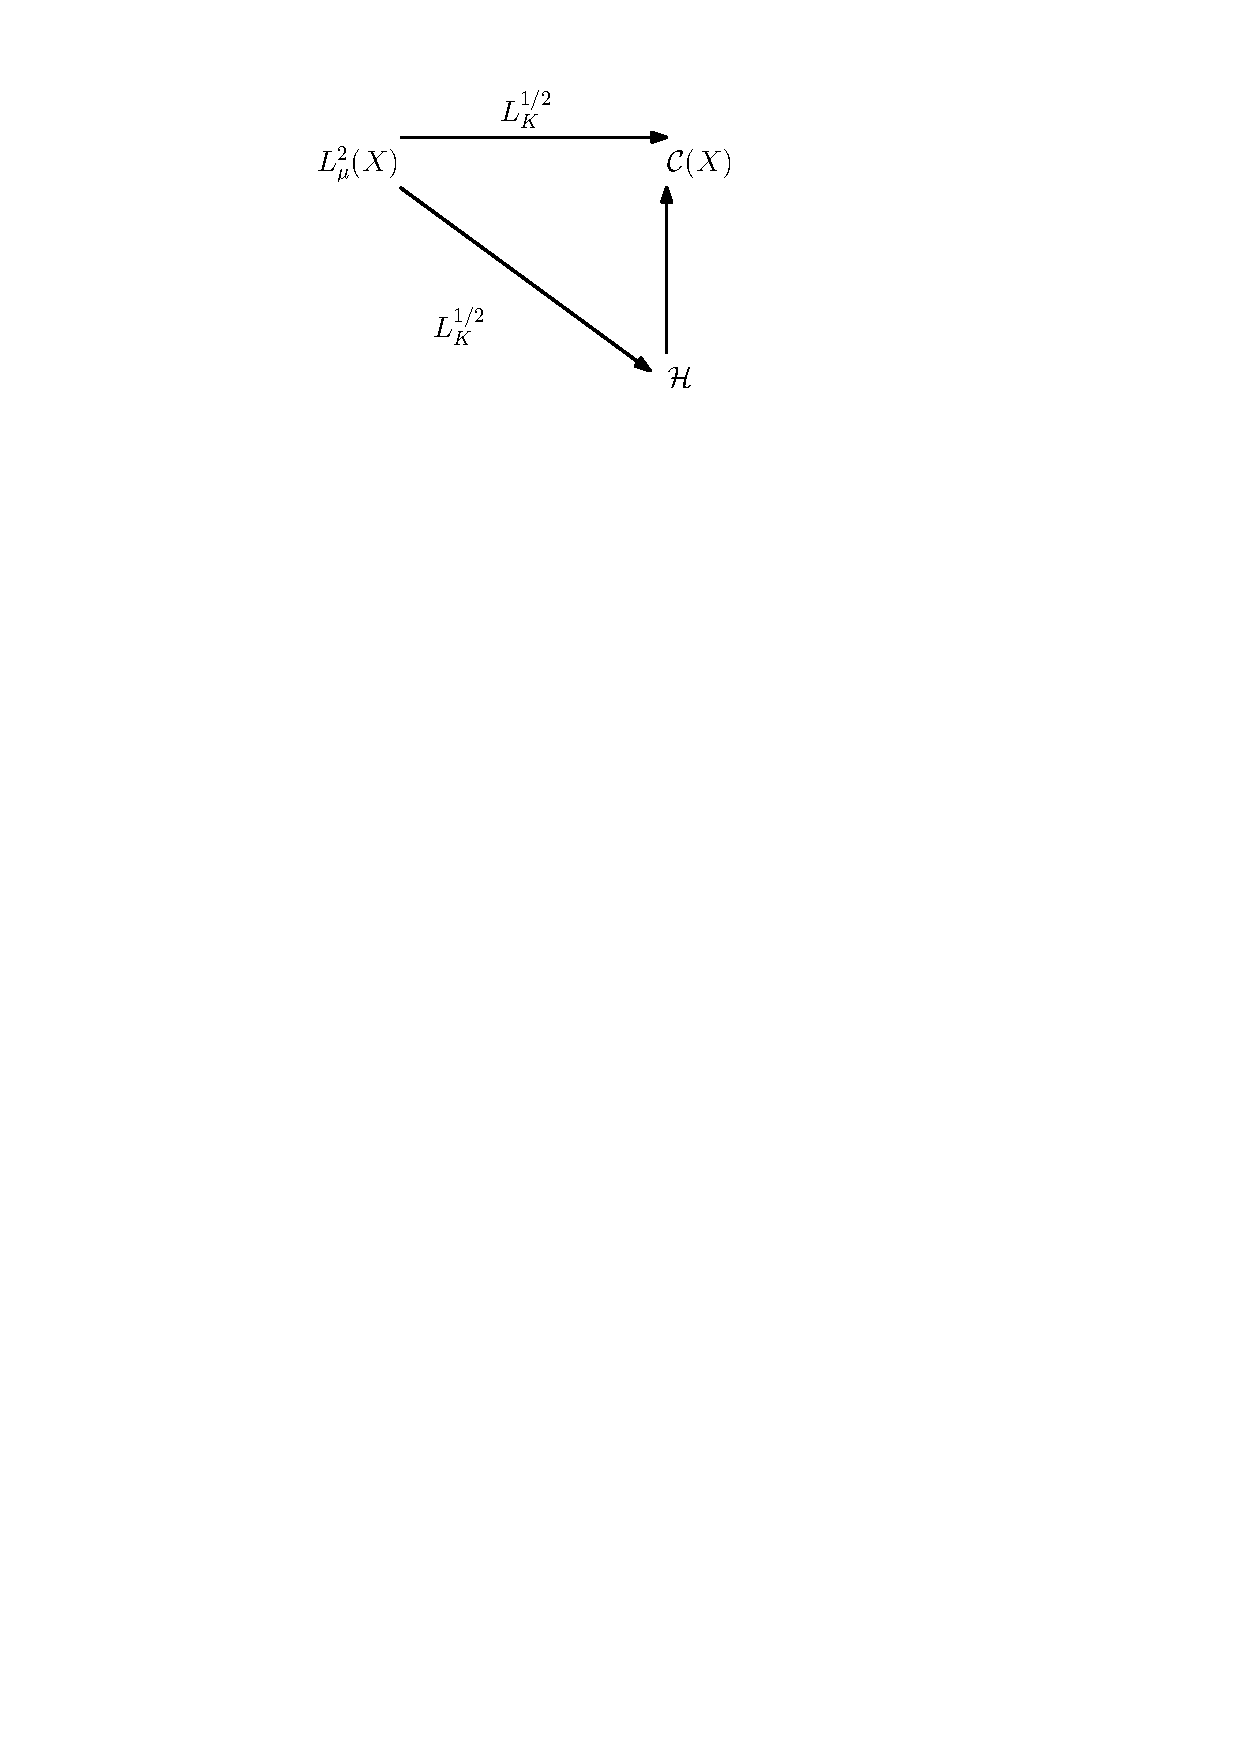
\includegraphics[width=3in]{images/Chap3_RKHS_isomorphism}
	\caption{Diagram illustrating the isomorphic transformations between $\clH$ and $L^2_\measure$.}
	\label{fig:rkhs_isomorphism}
\end{figure}

% $L_{K,C}$ emphasizes that the target is $\mathcal{C}(\state)$ and $I_K$ denotes the inclusion. If $\Kern$ is $\mathcal{C}^\infty$, then $I_K$ is compact. \anand{Gaussian kernel is $\mathcal{C}^\infty$}
$L_K$ is a self-adjoint, compact operator with eigenvalues $\reg_1 \geq \reg_2 \geq \cdots \geq 0$, with the corresponding normalized eigenfunctions $\{\phi_n\}_{n=1}^\infty$ forming an orthonormal basis for $L^2_\measure(\state)$. Mercer's theorem states that 
\begin{equation}
\Kern(x,x') = \sum_{n=1}^\infty \reg_n \phi_n(x) \phi_n(x'),
\end{equation}
where the series converges absolutely for each $x,x' \in \state$. The set $\{\sqrt{\reg_n}\phi_n\}_{n=1}^\infty$ forms an orthonormal basis for $\clH$. However, finding an eigenfunction feature representation for a kernel is challenging, except in special cases. 
 %
\chapter{Properties of the Gaussian Kernel -  RKHS}%
\label{a:gaussian_rkhs}

Of the many kernels being used, Gaussian kernel is the most widely used and often gives the best performance \cite{min10}. The study of the properties of the Gaussan kernel has received a lot of attention \cite{stehussco06, min10,micchaxuzha06}. The Gaussian kernel is a translation-invariant kernel given by,
\begin{equation}
\Kern_{\epsilon}(x,x') := \exp(-\|x - x'\|^2/ 4\epsilon) \qquad \forall x,x' \in \state,
\end{equation}
where $\epsilon$ is a parameter that defines the width of the kernel. An illustration of the Gaussian kernel for $\epsilon = 0.125$ and the corresponding Fourier transform is given in \Fig{fig:gaussian_kernel}. It may be seen that the Fourier transform decays exponentially fast for large values of $\omega$. The lack of high frequency components in the Gaussian kernel indicates that the functions belonging to the induced RKHS are smooth.  
\begin{figure}[htbp]
	\centering
	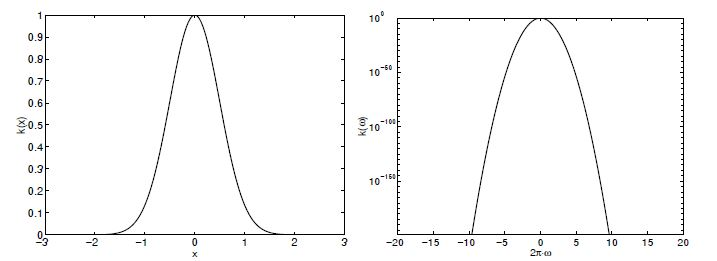
\includegraphics[width=6in]{images/Chap3_Gaussian_kernel}
	\caption{Gaussian kernel with $\epsilon = 0.125$ and its Fourier transform \cite{schsmo01}.}
	\label{fig:gaussian_kernel}
\end{figure}

Steinwart et al. in \cite{stehussco06} tries to answer questions like - which functions are contained in the RKHS induced by the Gaussian kernel, how the corresponding norms can be computed, and how the RKHS of different widths correlate to each other. 
In particular, RKHS of Gaussian kernels always have countable orthonormal bases. Theorem 3 of the paper gives the orthonormal basis functions for $\clH$ defined by the Gaussian kernel $\Kern_\epsilon$. It states that for $\epsilon >0$ and $n \in \mathbb{N}_0 := \mathbb{N} \cup \{0\}$, the sequence of functions $\{\phi_n : \Re \to \Re\}$ defined by,
\begin{equation}
\phi_n(x) := \sqrt{\frac{1}{(2\epsilon)^n n!}}x^n \exp(-x^2/4\epsilon).
\end{equation}
is an orthonormal basis for $\clH$.

Minh in \cite{min10} gives several properties of the RKHS induced by Gaussian kernels. Theorem 1 of the paper states that the RKHS $\clH$ induced by the standard Gaussian kernel is infinite dimensional, i.e. dim($\clH$) = $\infty$ and 
\begin{equation}
\clH := \Bigl\{ f = \exp(-x^2/4\epsilon) \sum_{n=0}^\infty w_n x^n: \|f\|^2_\clH = \sum_{k=0}^\infty (2\epsilon)^k k! \sum_{n=0}^k w_n^2 <\infty \Bigr\}
\end{equation}
Some of the salient properties of the Gaussian kernel RKHS are summarized below: 
\begin{arabnum}
	\item $\clH$ induced by the standard Gaussian kernel does not contain any polynomial on $\state$, including the non-zero constant function. 
	
	\item If $\state$ is compact, $\clH$ induced by the Gaussian kernel is dense in the space of $\mathcal{C}(\state)$ of continuous functions on $\state$.
	This means that given a continuous function $h(x)$, for all $\varepsilon >0$, we can find a function $g(x) \in \clH$ such that 
	\begin{equation}
	\|h(x) - g(x)\|_\infty \leq \epsilon \qquad \forall x \in \state
	\end{equation} 
	\item Let $\Kern_{\epsilon}(x,x') = \exp(-\frac{\|x-x'\|^2}{4\epsilon})$. The Hilbert space $\clH_\epsilon$ induced by $\Kern_\epsilon$ on $\state$ contains the function $\exp(-\frac{c \|x\|^2} {4 \epsilon})$ if and only if $0<c <2$. For example, $\exp(-\frac{\|x\|^2}{2 \epsilon}) \in \clH_{\epsilon/2}$, but  $\exp(-\frac{\|x\|^2}{2 \epsilon}) \notin \clH_{\epsilon}$. As $c=0$ is excluded, it validates the first property that constant functions do not belong to $\clH$.
	
	\item The functions in $\clH$ that are smooth are not necessarily integrable, as $\clH \notin L^1(\Re^n)$ for any $\epsilon >0$.  This implies that $L^1$ norm optimization or regularization is infeasible in $\clH$. This could still be done on subsets of finite linear combinations of the basis functions.
	
	
	\item Partial derivatives of the Gaussian kernel denoted as $\frac{\partial^n}{\partial x^n} \Kern_x \in \clH$. As a corollary, it can be shown that $t^n \Kern_x(t)\in\clH$. Additionally, for any polynomial $p(t)$, $p(t) \Kern_x(t) \in \clH$. An expression for the Hilbert space norm for kernel derivative of any order $d$ is also provided in \cite{min10}. 
\end{arabnum}

The paper by Michelli et al. \cite{micchaxuzha06} sets out to identify kernels with universal approximating property, i.e. given any compact set $\state$, any function $f \in \mathcal{C}(\state)$, there is a function $g \in \clH$ such that $\| f - g\|_{\infty} \leq \varepsilon$ holds for any $\varepsilon > 0$. Thus for any choice of compact set $\state$, the space $\clH$ is dense in $\mathcal{C}(\state)$ in the maximum norm. A kernel that satisfies this property is called the universal kernel. The paper discusses the characterization of universal kernels in terms of feature map representation of the kernel $\Kern$. It provides necessary and sufficient condition for $\Kern$ to have the universal approximation property in terms of its features. Under conditions provided in Theorem 17 of the paper, the standard Gaussian kernel is shown to be universal. 
 %
\chapter{Proof of Representer Theorem \Theorem{theorem:rep_theorem}}%
\label{a:reptheorem}

\begin{proof}
	From the definition of the RKHS $\clH$, any $f$ of the form:
	\[
	f \eqdef \sum_{i=1}^N  
	\beta_i \Kern(x_i,\cdot),
	\]
	is in $\clH$. 	
	Denote the linear subspace of $\clH$ made up of all such functions $f$ that are finite linear combinations of the kernel functions centered at $x_i$,
	\[
	\clH_\shortparallel := \Bigl\{f \in \clH\, |\, f = \sum_{i=1}^N  \beta_i \Kern(x_i,\cdot) \Bigr\},
	\]
	where $N$ ranges over $\mathbb{Z}_+$, and  each $\beta_i \in \Re$ for each $i$. Denote by $\clH_{\perp}$, the subspace of $\clH$ orthogonal to $\clH_\shortparallel$:
	\[
	\clH_\perp : = \{ \tilf \in \clH\,| \, \langle \tilf , f \rangle_\clH = 0 ,\, \forall f \in \clH_\shortparallel \}
	\]
	We can see that every $f \in \clH$ can be uniquely decomposed into a component lying within $\clH_\shortparallel$, denoted by $f_\shortparallel$ and a component lying within $\clH_\perp$, denoted by $f_\perp$.
	The $\clH$-norm can be written as,
	\[
	\Omega(\|f\|_\clH) = \Omega( \|f_\shortparallel + f_\perp\|_\clH) =\Omega( \sqrt{\|f_\shortparallel\|^2_\clH + \|f_\perp\|^2_\clH})  \geq \Omega(\|f_\shortparallel\|_\clH)
	\]
	The inequality is obtained from the fact that $\|f_\perp\|_\clH \geq 0$ and the function $\Omega(\cdot)$ is a strict monotone.
	This implies that the regularization term in \eqref{e:erm_rkhs} is minimized if $f$ lies in the subspace $\clH_\shortparallel$.
	Additionally, using reproducing property of the kernel $\Kern$,
	\[
	\begin{aligned}
	f(x_i) & =  \langle f \, , \Kern(x_i,.) \rangle_\clH\\
	&  = \langle f_\shortparallel\, , \Kern(x_i,.) \rangle_\clH + \langle f_\perp \, , \Kern(x_i,.) \rangle_\clH \\
	&  = \langle f_\shortparallel\, , K(x_i,.) \rangle_\clH \\
	&  = f_\shortparallel(x_i).
	\end{aligned}
	\]
	Therefore,
	\[
	L(x_i, f(x_i)) = L(x_i, f_\shortparallel(x_i))
	\]
	The empirical error term depends only on the component $f_\shortparallel$. Hence, the regularized objective function is minimized if $f_\reg^*$ lies within $\clH_\shortparallel$ and takes the form,
	\[
	f_\reg^*(x) = \sum_{i=1}^N  \beta_i^*  \Kern(x_i, x)
	\]
	This concludes the proof. 
\end{proof} %
\chapter{Generalization Error Bounds for least-squares regression on RKHS }%
\label{a:bousquet}
Here, we state some results on generalization error bounds for least-squares regression on RKHS obtained in \cite{boueli01} using the notions of stability of the algorithm.
Extensions to include ERM with gradient terms in the loss function is part of future work. 

Let $Z = X \times Y$ be the space of inputs and outputs and let $S = \{z_1 = (x_1, y_1), \cdots,z_N = (x_N,y_N)\}$ be a dataset of size $N$ drawn i.i.d. from an unknown distribution $\pr_{XY}$. Let $f:X \to Y$ be a function that maps from the input space $X$ to output space $Y$. A learning algorithm tries to learn the function $f_S$ from the given dataset $S$. 

The generalization error or expected risk is defined as:
\[
R(f) := \Expect_{z \sim \pr_{XY}} [c(f,z)]
\]
The empirical error of a function $f$ measured on the training set $S$ is:
\[
R_N(f) := \frac{1}{N}\sum_{i=1}^N c(f,z_i)
\]
Our aim is to obtain bounds on the random variable $R(f_S) - R_N(f_S)$. 

If $S = \{z_1,\dots, z_{i-1},z_i,z_{i+1},\dots z_N\}$, let us define a modified training set $S_i :=\{z_1,\dots, z_{i-1},z'_i,z_{i+1},\dots,z_N\}$ where the $i^{th}$ training sample $z_i$ is replaced by $z'_i$.

Uniform stability: A notion of uniform stability is defined for the algorithm as follows. If the training set $S$ is defined as above and $S_i$ be the training set where $i^{th}$ sample is removed, then the algorithm is $\beta$-stable if the following holds:
\[
\|c(f_S, z ) - c(f_{S_i},z)\|_{\infty} \leq \beta, \qquad \forall S \in Z^N, \forall z'_i, z \in Z,
\]
where $c(\cdot,\cdot)$ denotes the loss function. 
This condition implies stability of the algorithm in the sense that if a training sample from the original set is replaced by a new sample, the difference in cost is smaller than some constant $\beta$. 

\begin{lemma}
	For any symmetric learning algorithm we have for all $1\leq i \leq N$:
	\[
	\Expect_{S \sim \pr^N_{XY}} [R(f_S) - R_N(f_S)] = \Expect_{S,z'_i \sim \pr^{N+1}_{XY}} [c(f_S,z'_i) - c(f_{S_i}, z'_i)]
	\]
	\begin{proof}
		\[
		\Expect_{S \sim \pr^N_{XY}} [R_N(f_S)] = \frac{1}{N} \sum_{i=1}^N \Expect_{S \sim \pr^N_{XY}} [c(f_S, z_i)] = \Expect_{S \sim \pr^N_{XY}} [c(f_S, z_i)], \, \forall i \in \{1,\dots, N\}
		\]
		The above is true by symmetry and the i.i.d assumption. Now by simply renaming $z_i$ as $z'_i$,
		\[
		\Expect_{S \sim \pr^N_{XY}}[R_N(f_S)] = \Expect_{S_i \sim \pr^N_{XY}}[c(f_{S_i}, z'_i)]
		\]
		The expected risk term can be written as, 
		\[
		\Expect_{S \sim \pr^N_{XY}}[R(f_S)] = \Expect_{S,z'_i \sim \pr^{N+1}_{XY}} [c(f_S, z'_i)]
		\]
		Using this and the fact that the algorithm is $\beta$-stable, 
		\[
		\begin{aligned}
		\Expect_{S \sim \pr^N_{XY}} [R(f_S) - R_N(f_S)] &= \Expect_{S,z'_i\sim \pr^{N+1}_{XY}}[c(f_S,z'_i) - c(f_{S_i},z'_i)]\\
		&\leq \Expect_{S,z'_i\sim \pr^{N+1}_{XY}}[\beta] \\
		& = \beta
		\end{aligned}
		\]
	\end{proof}
\end{lemma}
Now, the next step is to prove that our algorithm of interest is $\beta$-stable for some value of $\beta$. 

\section{Application to Regularization in Hilbert Spaces}
Let $\clH$ be an RKHS induced by a kernel function $K$. Let us assume that $K$ is continuous and bounded, so that
\[
\kappa := \sup_{x \in X} \sqrt{K(x,x)} < \infty
\]
and therefore, by Cauchy-Schwarz inequality,
\begin{equation}
|f(x)| \leq \kappa \|f\|_\clH, \, \forall x \in X, \forall f \in \clH 
\label{e:cauchy_schwarz}
\end{equation}

\noindent $\sigma$-admissibility: A cost function $c(f(x),y)$ defined on $\clH \times Y$ is $\sigma$-admissible with respect to $\clH$ if $c$ is convex with respect to its first argument and the following condition holds
\[
|c(y_1, y') - c(y_2, y')| \leq \sigma |y_1 - y_2|, \, \forall y_1,y_2 \in \mathcal{D}, \forall y' \in Y,
\]
where $\mathcal{D} = \{y: \exists f \in \clH, \exists x \in X, f(x) = y\}$ is the domain of the first argument of $c$.  

\noindent \begin{theorem}
	If $l(f,z) = c(f(x),y)$ is $\sigma$-admissible with respect to $\clH$, then the learning algorithm defined by 
	\[
	A_S = \argmin_{g \in \clH} \frac{1}{N} \sum_{i=1}^N l(g, z_i) + \lambda \|g\|^2_\clH
	\]
	has uniform stability $\beta$ with respect to $l$ with
	\[
	\beta \leq \frac{\kappa^2 \sigma^2}{2 \lambda N}
	\]
\end{theorem}
The proof uses Lemma 20 in the paper that gives bounds on a general regularization term $N(g)$ that appears in the ERM. Here, we just state the result without the proof. 
 %
%\chapter{Expectation Maximization (EM) Algorithm for Gaussian Mixtures}
\label{a:em}

\begin{itemize}
\item E Step :

\begin{equation}
w^{(k)}(j|n)= \displaystyle \dfrac{w_{j}^{(k)}p_{j}(x^i;\mu_{j}^{(k)},\sigma_{j}^{(k)})}{ \displaystyle \sum_{j=0}^{m-1}w_{j}^{(k)} p_{j}(x^i;\mu_{j}^{(k)},\sigma_{j}^{(k)})}
\end{equation}
\item M Step :
\begin{equation}
\begin{aligned}
\mu_{j}^{(k+1)} &=  \dfrac{\displaystyle \sum_{n=1}^{N}w^{(k)}(j|n)x^i}{\displaystyle \sum_{n=1}^{N}w^{(k)}(j|n)}\\
\sigma_{j}^{(k+1)} &=  \sqrt{ \dfrac{\displaystyle \sum_{n=1}^{N}w^{(k)}(j|n)\|x^i-\mu_{j}^{(k+1)}\|^2}{\displaystyle \sum_{n=1}^{N}w^{(k)}(j|n)}}\\
w_{j}^{(k+1)} &=  \dfrac{1}{N} \displaystyle \sum_{n=1}^{N}w^{(k)}(j|n)
\end{aligned}
\end{equation}
\end{itemize} % %These files aren't included in the template
%\input{tex/appendixF} %
%\chapter{Proof of Representer Theorem \Theorem{theorem:rep_theorem}}%
\label{a:reptheorem}

\begin{proof}
	From the definition of the RKHS $\clH$, any $f$ of the form:
	\[
	f \eqdef \sum_{i=1}^N  
	\beta_i \Kern(x_i,\cdot),
	\]
	is in $\clH$. 	
	Denote the linear subspace of $\clH$ made up of all such functions $f$ that are finite linear combinations of the kernel functions centered at $x_i$,
	\[
	\clH_\shortparallel := \Bigl\{f \in \clH\, |\, f = \sum_{i=1}^N  \beta_i \Kern(x_i,\cdot) \Bigr\},
	\]
	where $N$ ranges over $\mathbb{Z}_+$, and  each $\beta_i \in \Re$ for each $i$. Denote by $\clH_{\perp}$, the subspace of $\clH$ orthogonal to $\clH_\shortparallel$:
	\[
	\clH_\perp : = \{ \tilf \in \clH\,| \, \langle \tilf , f \rangle_\clH = 0 ,\, \forall f \in \clH_\shortparallel \}
	\]
	We can see that every $f \in \clH$ can be uniquely decomposed into a component lying within $\clH_\shortparallel$, denoted by $f_\shortparallel$ and a component lying within $\clH_\perp$, denoted by $f_\perp$.
	The $\clH$-norm can be written as,
	\[
	\Omega(\|f\|_\clH) = \Omega( \|f_\shortparallel + f_\perp\|_\clH) =\Omega( \sqrt{\|f_\shortparallel\|^2_\clH + \|f_\perp\|^2_\clH})  \geq \Omega(\|f_\shortparallel\|_\clH)
	\]
	The inequality is obtained from the fact that $\|f_\perp\|_\clH \geq 0$ and the function $\Omega(\cdot)$ is a strict monotone.
	This implies that the regularization term in \eqref{e:erm_rkhs} is minimized if $f$ lies in the subspace $\clH_\shortparallel$.
	Additionally, using reproducing property of the kernel $\Kern$,
	\[
	\begin{aligned}
	f(x_i) & =  \langle f \, , \Kern(x_i,.) \rangle_\clH\\
	&  = \langle f_\shortparallel\, , \Kern(x_i,.) \rangle_\clH + \langle f_\perp \, , \Kern(x_i,.) \rangle_\clH \\
	&  = \langle f_\shortparallel\, , K(x_i,.) \rangle_\clH \\
	&  = f_\shortparallel(x_i).
	\end{aligned}
	\]
	Therefore,
	\[
	L(x_i, f(x_i)) = L(x_i, f_\shortparallel(x_i))
	\]
	The empirical error term depends only on the component $f_\shortparallel$. Hence, the regularized objective function is minimized if $f_\reg^*$ lies within $\clH_\shortparallel$ and takes the form,
	\[
	f_\reg^*(x) = \sum_{i=1}^N  \beta_i^*  \Kern(x_i, x)
	\]
	This concludes the proof. 
\end{proof}
%\chapter{Generalization Error Bounds for least-squares regression on RKHS }%
\label{a:bousquet}
Here, we state some results on generalization error bounds for least-squares regression on RKHS obtained in \cite{boueli01} using the notions of stability of the algorithm.
Extensions to include ERM with gradient terms in the loss function is part of future work. 

Let $Z = X \times Y$ be the space of inputs and outputs and let $S = \{z_1 = (x_1, y_1), \cdots,z_N = (x_N,y_N)\}$ be a dataset of size $N$ drawn i.i.d. from an unknown distribution $\pr_{XY}$. Let $f:X \to Y$ be a function that maps from the input space $X$ to output space $Y$. A learning algorithm tries to learn the function $f_S$ from the given dataset $S$. 

The generalization error or expected risk is defined as:
\[
R(f) := \Expect_{z \sim \pr_{XY}} [c(f,z)]
\]
The empirical error of a function $f$ measured on the training set $S$ is:
\[
R_N(f) := \frac{1}{N}\sum_{i=1}^N c(f,z_i)
\]
Our aim is to obtain bounds on the random variable $R(f_S) - R_N(f_S)$. 

If $S = \{z_1,\dots, z_{i-1},z_i,z_{i+1},\dots z_N\}$, let us define a modified training set $S_i :=\{z_1,\dots, z_{i-1},z'_i,z_{i+1},\dots,z_N\}$ where the $i^{th}$ training sample $z_i$ is replaced by $z'_i$.

Uniform stability: A notion of uniform stability is defined for the algorithm as follows. If the training set $S$ is defined as above and $S_i$ be the training set where $i^{th}$ sample is removed, then the algorithm is $\beta$-stable if the following holds:
\[
\|c(f_S, z ) - c(f_{S_i},z)\|_{\infty} \leq \beta, \qquad \forall S \in Z^N, \forall z'_i, z \in Z,
\]
where $c(\cdot,\cdot)$ denotes the loss function. 
This condition implies stability of the algorithm in the sense that if a training sample from the original set is replaced by a new sample, the difference in cost is smaller than some constant $\beta$. 

\begin{lemma}
	For any symmetric learning algorithm we have for all $1\leq i \leq N$:
	\[
	\Expect_{S \sim \pr^N_{XY}} [R(f_S) - R_N(f_S)] = \Expect_{S,z'_i \sim \pr^{N+1}_{XY}} [c(f_S,z'_i) - c(f_{S_i}, z'_i)]
	\]
	\begin{proof}
		\[
		\Expect_{S \sim \pr^N_{XY}} [R_N(f_S)] = \frac{1}{N} \sum_{i=1}^N \Expect_{S \sim \pr^N_{XY}} [c(f_S, z_i)] = \Expect_{S \sim \pr^N_{XY}} [c(f_S, z_i)], \, \forall i \in \{1,\dots, N\}
		\]
		The above is true by symmetry and the i.i.d assumption. Now by simply renaming $z_i$ as $z'_i$,
		\[
		\Expect_{S \sim \pr^N_{XY}}[R_N(f_S)] = \Expect_{S_i \sim \pr^N_{XY}}[c(f_{S_i}, z'_i)]
		\]
		The expected risk term can be written as, 
		\[
		\Expect_{S \sim \pr^N_{XY}}[R(f_S)] = \Expect_{S,z'_i \sim \pr^{N+1}_{XY}} [c(f_S, z'_i)]
		\]
		Using this and the fact that the algorithm is $\beta$-stable, 
		\[
		\begin{aligned}
		\Expect_{S \sim \pr^N_{XY}} [R(f_S) - R_N(f_S)] &= \Expect_{S,z'_i\sim \pr^{N+1}_{XY}}[c(f_S,z'_i) - c(f_{S_i},z'_i)]\\
		&\leq \Expect_{S,z'_i\sim \pr^{N+1}_{XY}}[\beta] \\
		& = \beta
		\end{aligned}
		\]
	\end{proof}
\end{lemma}
Now, the next step is to prove that our algorithm of interest is $\beta$-stable for some value of $\beta$. 

\section{Application to Regularization in Hilbert Spaces}
Let $\clH$ be an RKHS induced by a kernel function $K$. Let us assume that $K$ is continuous and bounded, so that
\[
\kappa := \sup_{x \in X} \sqrt{K(x,x)} < \infty
\]
and therefore, by Cauchy-Schwarz inequality,
\begin{equation}
|f(x)| \leq \kappa \|f\|_\clH, \, \forall x \in X, \forall f \in \clH 
\label{e:cauchy_schwarz}
\end{equation}

\noindent $\sigma$-admissibility: A cost function $c(f(x),y)$ defined on $\clH \times Y$ is $\sigma$-admissible with respect to $\clH$ if $c$ is convex with respect to its first argument and the following condition holds
\[
|c(y_1, y') - c(y_2, y')| \leq \sigma |y_1 - y_2|, \, \forall y_1,y_2 \in \mathcal{D}, \forall y' \in Y,
\]
where $\mathcal{D} = \{y: \exists f \in \clH, \exists x \in X, f(x) = y\}$ is the domain of the first argument of $c$.  

\noindent \begin{theorem}
	If $l(f,z) = c(f(x),y)$ is $\sigma$-admissible with respect to $\clH$, then the learning algorithm defined by 
	\[
	A_S = \argmin_{g \in \clH} \frac{1}{N} \sum_{i=1}^N l(g, z_i) + \lambda \|g\|^2_\clH
	\]
	has uniform stability $\beta$ with respect to $l$ with
	\[
	\beta \leq \frac{\kappa^2 \sigma^2}{2 \lambda N}
	\]
\end{theorem}
The proof uses Lemma 20 in the paper that gives bounds on a general regularization term $N(g)$ that appears in the ERM. Here, we just state the result without the proof. 

%\chapter{Expectation Maximization (EM) Algorithm for Gaussian Mixtures}
\label{a:em}

\begin{itemize}
\item E Step :

\begin{equation}
w^{(k)}(j|n)= \displaystyle \dfrac{w_{j}^{(k)}p_{j}(x^i;\mu_{j}^{(k)},\sigma_{j}^{(k)})}{ \displaystyle \sum_{j=0}^{m-1}w_{j}^{(k)} p_{j}(x^i;\mu_{j}^{(k)},\sigma_{j}^{(k)})}
\end{equation}
\item M Step :
\begin{equation}
\begin{aligned}
\mu_{j}^{(k+1)} &=  \dfrac{\displaystyle \sum_{n=1}^{N}w^{(k)}(j|n)x^i}{\displaystyle \sum_{n=1}^{N}w^{(k)}(j|n)}\\
\sigma_{j}^{(k+1)} &=  \sqrt{ \dfrac{\displaystyle \sum_{n=1}^{N}w^{(k)}(j|n)\|x^i-\mu_{j}^{(k+1)}\|^2}{\displaystyle \sum_{n=1}^{N}w^{(k)}(j|n)}}\\
w_{j}^{(k+1)} &=  \dfrac{1}{N} \displaystyle \sum_{n=1}^{N}w^{(k)}(j|n)
\end{aligned}
\end{equation}
\end{itemize}
 %Use this file if you have two or more appendices

%% The Editorial Office Requirements for the Table of Contents cause a significant problem
% in Latex if there is only one Appendix. The Appendix is no longer labeled "A" in the TOC
% but has the word "APPENDIX" placed in front of the title of the Appendix. This can be done
% without issue IF nothing needs to be numbered by LaTeX in the Appendix. Unfortunately, most of the time
% something needs to be numbered in that single Appendix. For this reason we have included
% this document which makes the changes needed to set up the format changes needed for a single appendix.

% There is no need to use the AppendixA.tex file just enter the appendix text after the chapter
% setup is completed


\appendix %

\chapter*{APPENDIX \\ THIS IS THE FIRST APPENDIX} %puts the chapter title at the beginning of the
% appendix without changing the chapter number

\addcontentsline{toc}{chapter}{APPENDIX: THIS IS THE FIRST APPENDIX} %puts the appendix title
% in the TOC correctly

\chaptermark{Appendix}
\markboth{Appendix}{Appendix}
\setcounter{chapter}{1} %These commands set the chapter counter properly and the appendix text
% is ready to go.

And the appendix text goes here. Lorem ipsum dolor sit amet, consectetuer
adipiscing elit. Maecenas eget magna. Aenean et lorem. Ut dignissim neque
at nisi. In hac habitasse platea dictumst. In porta ornare eros. Nunc eu ante.
In non est vehicula tellus cursus suscipit. Proin sed libero. Sed risus
enim, eleifend in, pellentesque ac, nonummy quis, nulla. Phasellus
imperdiet libero nec massa. Ut sapien libero, adipiscing eu,
volutpat porttitor, ultricies eget, nisi. Sed odio. Suspendisse
potenti. Duis dolor augue, viverra id, porta in, dignissim id, nisl.
Vivamus blandit cursus eros. Maecenas sit amet urna sit amet orci
nonummy pharetra.

Praesent cursus nibh et mauris. In aliquam felis sit amet ligula.
Nulla faucibus nisl eget nisl. Aliquam tincidunt. Mauris eget elit
sed massa luctus posuere. Pellentesque suscipit. In odio urna,
semper ut, convallis ut, porta et, nibh. Nulla sodales metus nec
velit posuere gravida. Cras tristique. Etiam urna risus, accumsan
ut, placerat sed, iaculis id, est.

Nullam mi. Pellentesque habitant morbi tristique senectus et netus
et malesuada fames ac turpis egestas. Duis vitae metus in massa
hendrerit rhoncus. Fusce tortor justo, laoreet eu, facilisis at,
gravida et, felis. Donec imperdiet mollis erat. Integer tempus nulla
ac lorem. Fusce porttitor. Aenean quis arcu. Morbi consectetuer, leo
eu mollis elementum, urna massa malesuada risus, euismod tempor
lorem elit ut mauris. Cras elit orci, facilisis ac, mattis iaculis,
cursus ac, augue. Donec eget nisl. Pellentesque fermentum sodales
nibh. Vivamus non risus. Donec est libero, tincidunt sit amet,
pretium vitae, blandit sed, tellus. Nunc diam risus, interdum sed,
laoreet quis, varius ac, turpis. In et purus eget nibh vehicula
rhoncus. Aenean et neque. Praesent nisl nisi, tempus quis, nonummy
ac, auctor a, neque. Suspendisse et metus. Suspendisse non metus eu
mauris auctor sagittis.
 %Use this file if you have one and only one appendix

%------------------------------------------%

% Make List of References (BibTeX implemented using the Natbib package)
% un-comment your preferred bibliography style and replace the
% bibliography file "sample" with the name of your .bib file
% REMEMBER!!! If you want un-numbered references comment the Natbib package with
% The numbered options in the packages.tex file and un-comment the package with the authoryear option
% See the included pdfs of the various styles to see the differences.
% The citation style differences are from the \citet{key} and \citep{key} commands
% More options are available; see the Natbib documentation for details


\bibliography {bib/AnandPhDRefMaster, bib/strings}
% You can have more than one library of references - put the .bib file
% in the bib folder and call it here
%------------------------------------------%

% Bio Sketch is required and should be in third person, past tense%
% Just type your bio in between the brackets
\biography{%
This section is where your biographical sketch is typed in the
\url{bio.tex} file. It should be in third person, past tense. Do not put 
personal details such as your birthday in the file. Again, to make a full paragraph 
you must write at least three sentences.}


%------------------------------------------%

\end{document}

%-------------------------------------------------------------------------------------------------------%
